\documentclass[11pt]{book}
\oddsidemargin 0in
\evensidemargin 0in
\marginparwidth 0in
\textheight 8in
\textwidth 6.5in
\topmargin 0in
\headheight 14pt
\usepackage{amssymb,amsmath,amsthm,fancyhdr,supertabular,longtable,hhline,mathtools}
\usepackage{colortbl}
\usepackage{import, multicol,boxedminipage}
\usepackage{chapterfolder}
\usepackage[metapost,truebbox]{mfpic}
\usepackage[pdflatex]{graphicx}
\usepackage{makeidx}
\usepackage[colorlinks, hyperindex, plainpages=false, linkcolor=blue, urlcolor=blue, pdfpagelabels]{hyperref}
\usepackage[all]{hypcap}
\usepackage{cancel}
\usepackage{sectsty}
\usepackage{textcomp}
\allsectionsfont{\mdseries \scshape}
\definecolor{ResultColor}{gray}{0.9}
\theoremstyle{definition}  % this prevents the text in definitions, theorems, and corollaries from being italicized
\newtheorem{defn}{\sc Definition}[chapter]
\newtheorem*{defnrecall}{\sc Definition}
\newtheorem{thm}{\sc Theorem}[chapter]
\newtheorem{cor}[thm]{\sc Corollary}
\newtheorem{eqn}{\sc Equation}[chapter]
\newtheorem{ex}{\sc Example}[section]
\newtheorem{fig}{\sc Figure}[chapter]
\setlength{\parindent}{0in}
\newcommand{\bbm}{\begin{boxedminipage}{6.41in}}
\newcommand{\ebm}{\end{boxedminipage}}
\newcommand{\ds}{\displaystyle}
\usepackage{array}
\setlength{\extrarowheight}{2pt}
\allowdisplaybreaks[2]
\allsectionsfont{\mdseries \scshape}
%Below is for Helvetica (scaled): 
\usepackage[scaled=.92]{helvet}   
\renewcommand{\familydefault}{\sfdefault}  %makes the text of the book sans serif
\usepackage[helvet]{sfmath}  %makes the math in the book sans serif
\allsectionsfont{\sffamily}  %makes the chapter and section titles sans serif

\makeatletter
\newcases{mycases}{\quad}{%
  \hfil$\m@th\displaystyle{##}$}{$\m@th\displaystyle{##}$\hfil}{\lbrace}{.}
\makeatother

\begin{document}
\newcounter{HW}
\newcounter{HWindent}
\renewcommand{\textinterrobang}{$! \! \! ?$}


\chapter{\sc First Steps into Calculus}

\section{A (more) Formal Introduction to Limits}

\documentclass{ximera}

\begin{document}
	\author{Stitz-Zeager}
	\xmtitle{TITLE}


\mfpicnumber{1}

\opengraphsfile{IntroLimits}

\setcounter{footnote}{0}

\label{IntroLimits}

In this chapter, we take some more steps towards\footnote{into?} Calculus.  We first revisit the  concept of \index{limit}\textbf{limit} .  We've primarily used limits as a way to analyze and codify function behavior in places where we simplify could not evaluate the function.\footnote{Whether it be describing end behavior as $x \rightarrow  - \infty$  or $x \rightarrow  \infty$ or places where we'd be dividing by `$0$.'}  We first focus on how the concept is expressed graphically.

\subsection{Limits from Graphs}
\label{limitsfromgraphs}

Even though we didn't introduce the limit concept or notation until Chapter \ref{PolynomialFunctions}, we first encounter the underlying concept much earlier.  Recall in  Example \ref{functiongraphex01} we were given the graph of a function $w = F(v)$:

\begin{center}

\begin{tikzpicture}[scale=0.8]
  % Axes
  \draw[->] (-5,0) -- (5.2,0) node[below right] {\scriptsize $v$};
  \draw[->] (0,-5) -- (0,5.2) node[above right] {\scriptsize $w$};

  % Axis ticks
  \foreach \x in {-4,-3,-2,-1,1,2,3,4}
    \draw (\x,0.1) -- (\x,-0.1);
  \foreach \y in {-4,-3,-2,-1,1,2,3,4}
    \draw (0.1,\y) -- (-0.1,\y);

  % Custom x-axis labels
  \node[below] at (-1,0) {\scriptsize $-1$};
  \node[below] at (1,0)  {\scriptsize $1$};
  \node[below] at (4,0)  {\scriptsize $4$};

  % Custom y-axis labels
  \node[left] at (0,-3) {\scriptsize $-3$};
  \node[left] at (0,-2) {\scriptsize $-2$};
  \node[left] at (0,-1) {\scriptsize $-1$};
  \node[left] at (0,1)  {\scriptsize $1$};
  \node[left] at (0,2)  {\scriptsize $2$};
  \node[left] at (0,3)  {\scriptsize $3$};
  \node[left] at (0,4)  {\scriptsize $4$};

  % Labels for specific points
  \node[below] at (2,0) {\scriptsize $(2,0)$};
  \node[below] at (-2,0) {\scriptsize $(-2,0)$};
  \node[below] at (0,-4) {\scriptsize $(0,-4)$};
  \node[below right] at (1,-3) {\scriptsize $(1,-3)$};

  % Function plot: w = v^2 - 4
  \draw[thick,domain=-2:3,samples=100] plot (\x,{\x*\x-4});

  % Points
  \filldraw ( -2, 0) circle (2pt);
  \filldraw (  0,-4) circle (2pt);
  \filldraw (  2, 0) circle (2pt);

  \draw (1,-3) circle (2pt); % unfilled point
\end{tikzpicture}

% \begin{mfpic}[15]{-5}{5}{-5}{5}
% \axes
% \tlabel[cc](5,-0.5){\scriptsize $v$}
% \tlabel[cc](0.5,5){\scriptsize $w$}
% \tlabel[cc](2.5,-0.5){\scriptsize $(2,0)$}
% \tlabel[cc](-3,-0.5){\scriptsize $(-2,0)$}
% \tlabel[cc](1,-4.25){\scriptsize $(0,-4)$}
% \tlabel[cc](2,-3.25){\scriptsize $(1,-3)$}
% \xmarks{-4 step 1 until 4 }
% \ymarks{-4 step 1 until 4}
% \tlpointsep{5pt}
% \scriptsize
% \axislabels {x}{{$-1 \hspace{7pt}$} -1, {$1$} 1, {$4$} 4}
% \axislabels {y}{{$-3$} -3,{$-2$} -2,  {$-1$} -1, {$1$} 1, {$2$} 2, {$3$} 3, {$4$} 4}
% \normalsize
% \penwd{1.25pt}
% \arrow \function{-2,3,0.1}{x**2-4}
% \point[4pt]{(-2,0), (0,-4), (2,0)}
% \pointfillfalse
% \point[4pt]{(1,-3)}
% \end{mfpic} 

\end{center}


The hole in the graph tells us that even though $F(1)$ is undefined, we'd \textbf{expect} $F(1)$ to be $-3$ based on what's happening with the graph \textbf{near} the point $(1,-3)$.  Using limit notation, we'd write  $\ds{\lim_{v \rightarrow 1} F(v) = -3}$.  We take a moment below to better define what we mean when use the limit notation.

\medskip

%% \colorbox{ResultColor}{\bbm

\begin{definition} \label{informallimitdefn} \textbf{Informal Definition of Limit:}  Given a function $f$ defined on an open interval containing $x=a$, except possibly at $x=a$, the notation $\ds{\lim_{x \rightarrow a} f(x) = L}$,\index{limit ! informal definition} means as input values, $x$, approach\footnote{ignoring what is happening at $x=a$} the number $a$, the output values, $f(x)$, approach the number $L$.  The notation ` $\ds{\lim_{x \rightarrow a} f(x) = L}$'  is read read `the \textbf{limit} as $x$ approaches $a$ of $f(x)$ equals $L$.' 
\end{definition}

%% \ebm}


\medskip


Some remarks about Definition \ref{informallimitdefn} are in order.  Note that the business about $f$ being defined on `an open interval containing $x=a$'  is there to guarantee that we have the appropriate `room' for inputs $x$ to approach $a$ from either direction.\footnote{We'll get to `one-sided' limits here shortly.}  (For now, we'll just assume we all understand what the word `approach' means in this context and let a Calculus class explain how this is more precisely codified mathematically.)

\medskip 

The phrase  `except possibly at $x=a$' which immediately follows means the limit doesn't concern itself with what is actually happening at $x=a$.  The function  $f$ may or may not be defined at $x = a$.  Indeed,  if  $\ds{\lim_{x \rightarrow a} f(x) = L}$, $f(a)$ could be $L$, $f(a)$  could be a number different than $L$ or $f(a)$ could not be defined. 

\medskip

 This drives home the principle difference between the precalculus notion of `$f(a)$' and the Calculus notion of  `$\ds{\lim_{x \rightarrow a} f(x)}$':  `$\ds{\lim_{x \rightarrow a} f(x)}$' is what we \textbf{expect} $f(a)$ to be - which may or may not agree with what $f(a)$, if $f(a)$ is even defined. 

\medskip

For example, using the graph from Example \ref{functiongraphex01}, we write $\ds{\lim_{v \rightarrow 0} F(v) = -4}$ since as $v \rightarrow 0$, we see $w = F(v) \rightarrow -4$.  In this particular case, $F(0) = -4$ so we get from $F$ at $v=0$ what we expect to get.\footnote{This is another way to describe the notion of \index{continuity}\textbf{continuity}.  (See Definition \ref{continuousdefn}.)}

\medskip

For another example, consider the graphs of the functions $f$, $g$, and $h$ below near $x = 2$. Through a precalculus lens, each of these functions is different at $x = 2$:   $f(2) = 3$, $g(2) = 1$, and $h(2)$ is undefined.  Through a Calculus lens, however, all three of these functions are behaving identically as  $x$ approaches $2$:   $\ds{\lim_{x \rightarrow 2} f(x) = 3}$, $\ds{ \lim_{x \rightarrow 2} g(x)= 3}$, and $\ds{\lim_{x \rightarrow 2} h(x) = 3}$.


\begin{center}

\begin{tabular}{ccc}

 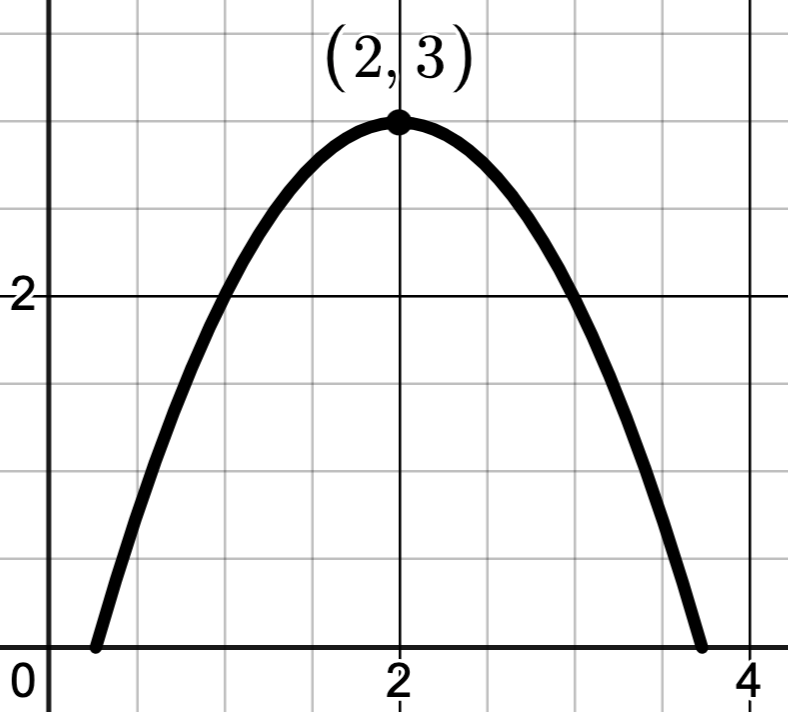
\includegraphics[width=2in]{./IntroLimitsGraphics/limitgrapha.png} &  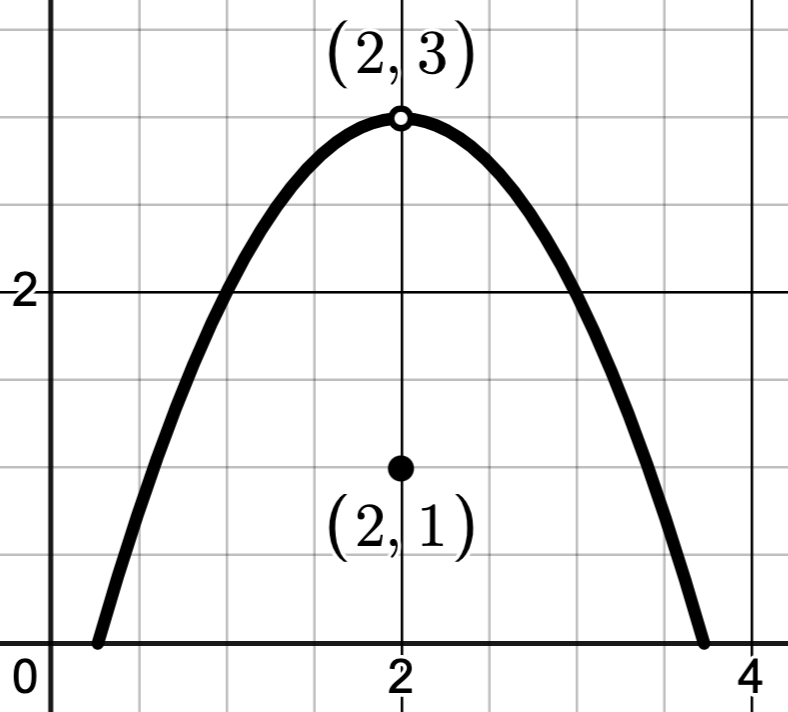
\includegraphics[width=2in]{./IntroLimitsGraphics/limitgraphc.png} &  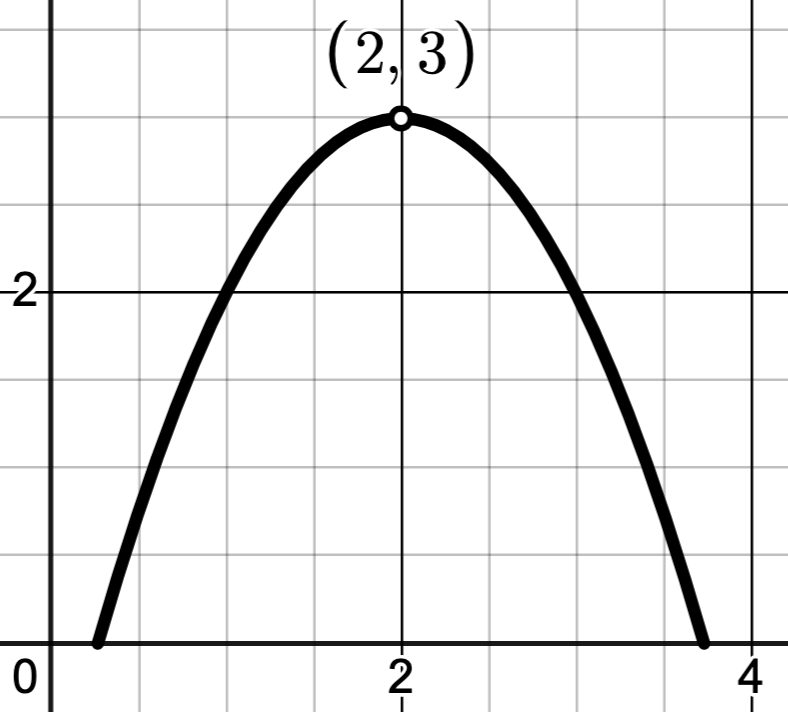
\includegraphics[width=2in]{./IntroLimitsGraphics/limitgraphb.png} \\
 
 $y = f(x)$ & $y = g(x)$ & $y = h(x)$ \\
 
 \end{tabular}
 
 \end{center}
 

 Next let's head to Section \ref{ConstantandLinearFunctions} and revisit Example \ref{piecewiseconstantex} in a piecewise-defined function is used to model matinee admission prices at a local theater:
    
   \begin{center}

\begin{mfpic}[25]{-1}{6}{-1}{5}
\axes
\tlabel[cc](6,-0.5){\scriptsize $A$}
\tlabel[cc](0.5,5){\scriptsize $y$}
\xmarks{1,2,3,4,5}
\ymarks{1,2,3,4}
\scriptsize
\tlabel[cc](-1, 2.875){$(0, 5.75)$}
\tlabel[cc](0.8, 4){$(6, 7.25)$}
\tlabel[cc](5, 2.5){$(50, 5.75)$}
\tlpointsep{4pt}
\axislabels {x}{ {$10$} 1, {$20$} 2, {$30$} 3, {$40$} 4, {$50$} 5}
\axislabels {y}{{$2$} 1, {$4$} 2,   {$8$} 4}
\penwd{1.25pt}
\polyline{( 0,2.875), (0.6,2.875)}
\polyline{( 0.6,3.625), (5,3.625)}
\arrow \polyline{(5,2.875), (6, 2.875)}
\point[3pt]{(0,2.875), (5, 2.875),( 0.6,3.625) }
\pointfillfalse
\point[3pt]{(0.6,2.875), (5,3.625)}
\tcaption{ $y = p(A) = \begin{mycases} 
      5.75 &  \text{if $0 \leq A < 6$ or $A \geq 50$} \\
      7.25  & \text{if $6 \leq A < 50$} \\
   \end{mycases}$}
\normalsize
\end{mfpic} 

\end{center}

What can be said about $\ds{ \lim_{A \rightarrow 6} p(A)}$?   Remember, $\ds{ \lim_{A \rightarrow 6} p(A)}$ is what we would \textbf{expect} $p(6)$ to be by analyzing $p$ as $A \rightarrow  6$, ignoring what is happening at $A=6$.  If $A<6$,  $p(A)$ is always $5.75$, so, based on this information, we'd \textbf{expect} $p(6)$ to be $5.75$.   If $A>6$, then  $p(A)$ is always $7.25$, so we'd \text{expect} $p(6)$ to be $7.25$.  Since Definition  \ref{informallimitdefn} requires the $p(A)$ values to approach a \textbf{single} value $L$ as $A \rightarrow 6$, we'd say in this case that   $\ds{ \lim_{A \rightarrow 6} p(A)}$ does not exist.  

\medskip

Even though $\ds{ \lim_{A \rightarrow 6} p(A)}$ does not exist, we've used so-called `one-sided' limit notation in Chapters \ref{RationalFunctions} and \ref{RootRadicalPowerFunctions} which we can apply here.  Specifically, we write  $\ds{\lim_{A \rightarrow 6^{-}} p(A) = 5.75}$ and  $\ds{\lim_{A \rightarrow 6^{+}} p(A) = 7.25}$ to more precisely record the behavior of $p$ as we approach $ A = 6$ from either direction.\footnote{Note that $\ds{\lim_{A \rightarrow 6^{+}} p(A) = 7.25 = p(6)}$ in this case.  So at least we `get' what we `expect to get' when approaching $6$ from the right.}

\medskip

%% \colorbox{ResultColor}{\bbm

\begin{definition} \label{onesidedimitdefn} \textbf{One-sided Limits:}  

\begin{itemize}

\item If $f$ is defined on an open interval for $x<a$ except possibly at $x=a$, the notation  $\ds{\lim_{x \rightarrow a^{-}} f(x) = L}$,\index{limit ! informal definition ! from the left} read `the \textbf{limit} as $x$ approaches $a$ \textbf{from the left} of $f(x)$ equals $L$' means as input values, $x$, $x < a$, approach the number $a$ (ignoring what is happening at $x=a$), the output values, $f(x)$, approach the number $L$. 

\item If $f$ is defined on an open interval for $x>a$ except possibly at $x=a$, the notation  $\ds{\lim_{x \rightarrow a^{+}} f(x) = L}$,\index{limit ! informal definition ! from the right} read `the \textbf{limit} as $x$ approaches $a$ \textbf{from the right} of $f(x)$ equals $L$' means as input values, $x$, $x > a$, approach the number $a$ (ignoring what is happening at $x=a$), the output values, $f(x)$, approach the number $L$. 


\end{itemize}

\end{definition}

%% \ebm}


\medskip

In order for the (two-sided) limit to exist, both one-sided limits need to exist, be equal, and vice-versa.  This is recorded in the following theorem.

\medskip

%% \colorbox{ResultColor}{\bbm

\begin{theorem}  \label{onesidedlimit}  Given a function $f$ defined on an open interval containing $x=a$, except possibly at $x=a$,  $\ds{\lim_{x \rightarrow a} f(x) = L}$ if and only if $\ds{\lim_{x \rightarrow a^{-}} f(x) = L}$ and $\ds{\lim_{x \rightarrow a^{+}} f(x) = L}$.


\end{theorem}
%% \ebm}

\medskip

It's time for an example.

\begin{example} \label{limitfromgraphex} Use the \textbf{complete} graph\footnote{Recall this means this is the entire graph of $f$.  There's nothing hidden offscreen.} of $y = f(x)$ below to answer the following questions.





\begin{center}

 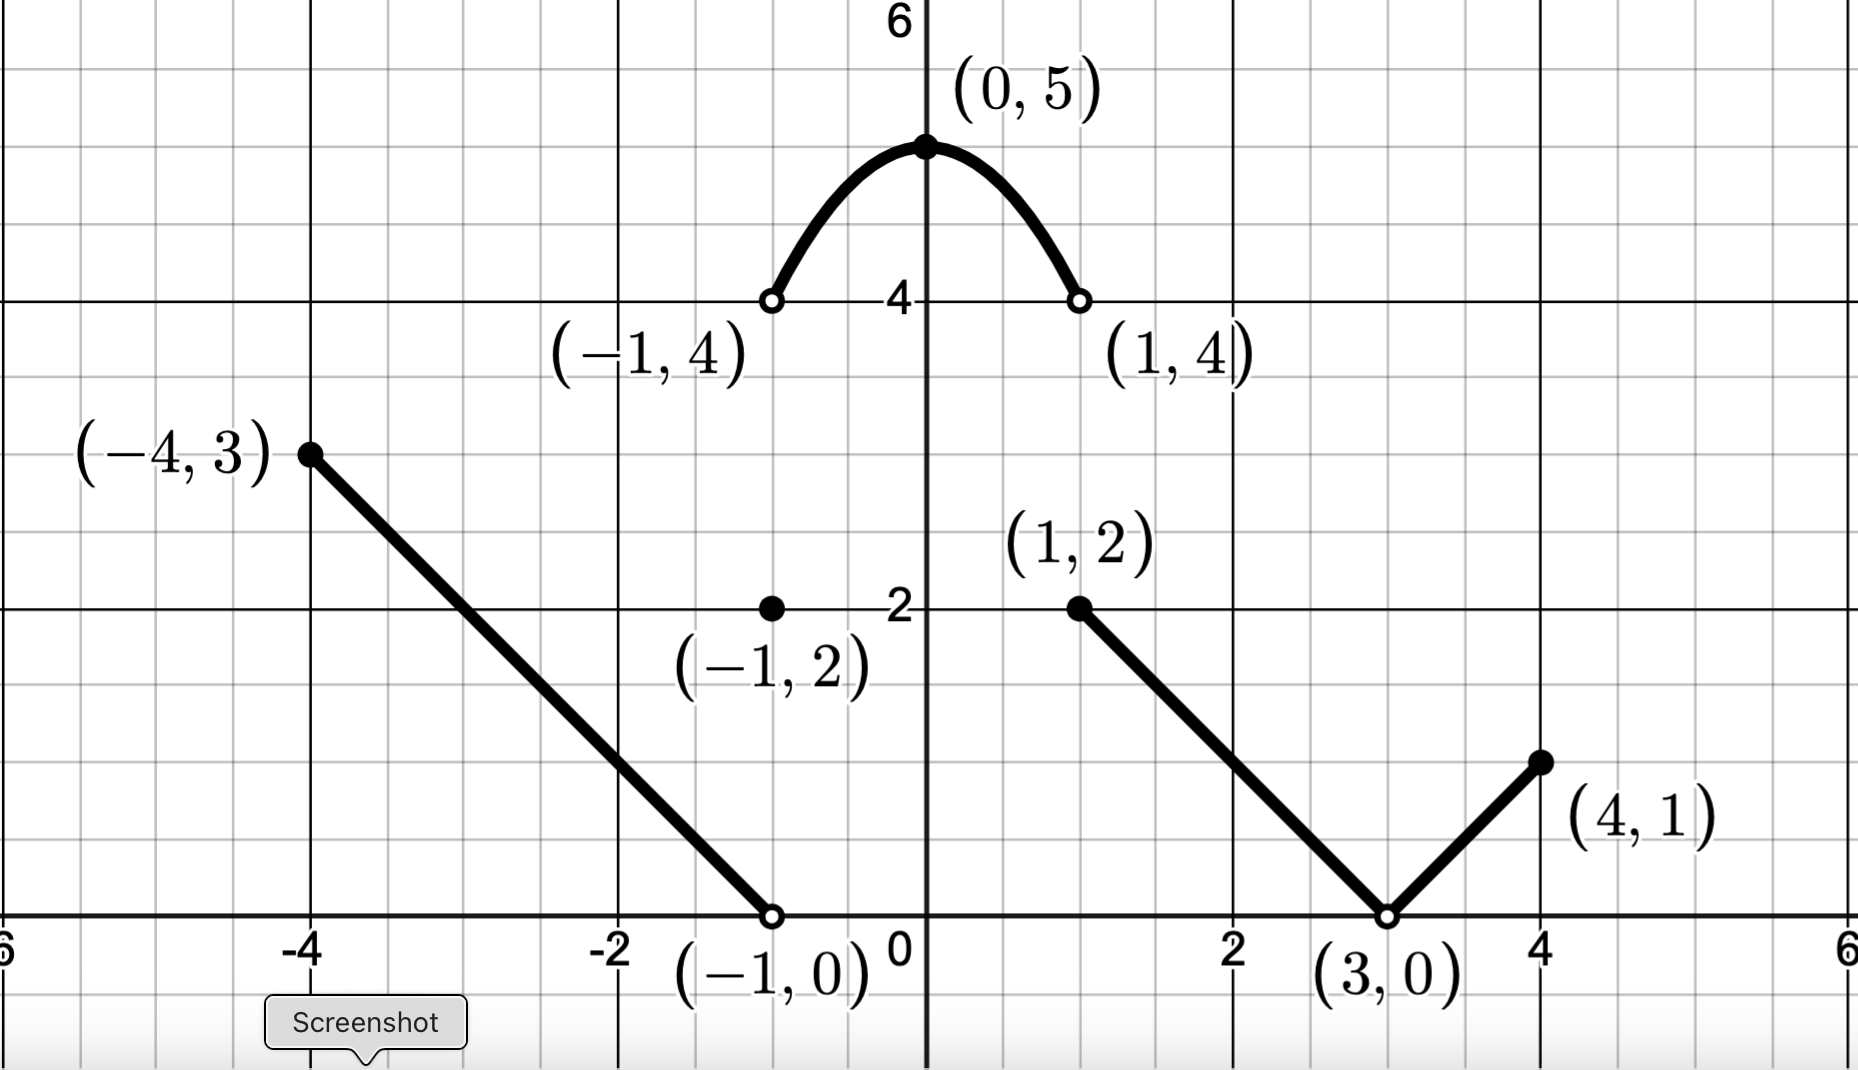
\includegraphics[width=5.5in]{./IntroLimitsGraphics/LimitfromGraphEx.png}
 
  \end{center}
  
  

  
  
\begin{enumerate}

\item  State the domain and range of $f$ using interval notation.


\item  Find the following values. Explain your reasoning.

 \begin{multicols}{4}
 
 \begin{itemize}
 
 \item $f(-1)$
 
 \item  $\ds{ \lim_{x \rightarrow -1^{-}} f(x)}$
 
  \item  $\ds{ \lim_{x \rightarrow -1^{+}} f(x)}$
 
  \item  $\ds{ \lim_{x \rightarrow -1} f(x)}$
 
 \end{itemize}
 
  \end{multicols}
 
\smallskip
 
  \begin{multicols}{4}
 
 \begin{itemize}
 
 \item $f(1)$
 
 \item  $\ds{ \lim_{x \rightarrow 1^{-}} f(x)}$
 
  \item  $\ds{ \lim_{x \rightarrow 1^{+}} f(x)}$
 
   \item  $\ds{ \lim_{x \rightarrow 1} f(x)}$
 
 \end{itemize}
 
  \end{multicols}
 
\smallskip
 
 \begin{multicols}{4}
 
 \begin{itemize}
 
 \item $f(0)$
 
 \item  $\ds{ \lim_{x \rightarrow 0^{-}} f(x)}$
 
  \item  $\ds{ \lim_{x \rightarrow 0^{+}} f(x)}$
 
  \item  $\ds{ \lim_{x \rightarrow 0} f(x)}$
 
 \end{itemize}
 
  \end{multicols}
 
\smallskip
 
  \begin{multicols}{4}
 
 \begin{itemize}
 
 \item $f(3)$
 
 \item  $\ds{ \lim_{x \rightarrow 3^{-}} f(x)}$
 
  \item  $\ds{ \lim_{x \rightarrow 3^{+}} f(x)}$
 
   \item  $\ds{ \lim_{x \rightarrow 3} f(x)}$
 
 \end{itemize}
 
  \end{multicols}
 
\smallskip

\item  Explain why  $\ds{ \lim_{x \rightarrow -4} f(x)}$ does not exist and find  $\ds{ \lim_{x \rightarrow -4^{+}} f(x)}$
\smallskip

\item  Explain why  $\ds{ \lim_{x \rightarrow 4} f(x)}$ does not exist and find  $\ds{ \lim_{x \rightarrow 4^{-}} f(x)}$

\end{enumerate}


{\bf Solution.}

\begin{enumerate}

\item  Projecting the graph of $f$ to the $x-$axis, we find that everything from $-4$ to $4$, inclusive, is covered except for $x = 3$.  Hence the domain is $[-4,3) \cup (3,4]$.  When projecting the graph of $f$ to the $y$-axis, we see everything between $0$ and $3$ is covered (excluding $0$ and including $3$) then everything between $4$  and $5$ is covered (excluding $4$ and including $5$).  Hence the range is $(0,3] \cup (4,5]$.


\item  \begin{itemize}  \item  Regarding $x = -1$:  since the point $(-1,2)$ is on the graph of $f$, we know $f(-1) =2$.  To determine  $\ds{ \lim_{x \rightarrow -1^{-}} f(x)}$, we see that the graph to the left of $x = -1$ is headed towards the point $(-1,0)$ as $x$ approaches $-1$.  Hence,  $\ds{ \lim_{x \rightarrow -1^{-}} f(x)= 0}$.  To determine  $\ds{ \lim_{x \rightarrow -1^{+}} f(x)}$, we see that the graph to the right of $x = -1$  is headed towards the point $(-1,4)$ as $x$ approaches $-1$.  Hence,  $\ds{ \lim_{x \rightarrow -1^{+}} f(x)= 4}$.    Since $\ds{ \lim_{x \rightarrow -1^{-}} f(x)}$ and $\ds{ \lim_{x \rightarrow -1^{+}} f(x)}$ are different,  $\ds{ \lim_{x \rightarrow -1} f(x)}$ does not exist.

\item  Regarding $x = 1$:  since the point $(1,2)$ is on the graph of $f$, we know $f(1) =2$.  To determine  $\ds{ \lim_{x \rightarrow 1^{-}} f(x)}$, we see that the graph to the left of $x = 1$ is headed towards the point $(1,4)$ as $x$ approaches $1$.  Hence,  $\ds{ \lim_{x \rightarrow 1^{-}} f(x)= 4}$.  To determine  $\ds{ \lim_{x \rightarrow 1^{+}} f(x)}$, we see that the graph to the right of $x = 1$  is headed towards the point $(1,2)$ as $x$ approaches $1$.  Hence,  $\ds{ \lim_{x \rightarrow 1^{+}} f(x)= 2}$.    Since $\ds{ \lim_{x \rightarrow 1^{-}} f(x)}$ and $\ds{ \lim_{x \rightarrow 1^{+}} f(x)}$ are different,  $\ds{ \lim_{x \rightarrow 1} f(x)}$ does not exist.

\item  Regarding $x = 0$:  since the point $(0,5)$ is on the graph of $f$, we know $f(0) =5$.  To determine  $\ds{ \lim_{x \rightarrow 0^{-}} f(x)}$, we see that the graph to the left of $x = 0$ is headed towards the point $(0,5)$ as $x$ approaches $0$.  Hence,  $\ds{ \lim_{x \rightarrow 0^{-}} f(x)= 5}$.  To determine  $\ds{ \lim_{x \rightarrow 0^{+}} f(x)}$, we see that the graph to the right of $x = 0$  is headed towards the point $(0,5)$ as $x$ approaches $0$.  Hence,  $\ds{ \lim_{x \rightarrow 0^{+}} f(x)= 5}$.    Since $\ds{ \lim_{x \rightarrow 0^{-}} f(x)}$ and $\ds{ \lim_{x \rightarrow 0^{+}} f(x)}$ are both $5$,  $\ds{ \lim_{x \rightarrow 0} f(x) = 5}$.


\item  Regarding $x = 3$:  since there is no point on the graph of $f$ with an $x$-coordinate of $3$, $f(3)$ is undefined.  To determine  $\ds{ \lim_{x \rightarrow 3^{-}} f(x)}$, we see that the graph to the left of $x = 3$ is headed towards the point $(3,0)$ as $x$ approaches $3$.  Hence,  $\ds{ \lim_{x \rightarrow 3^{-}} f(x)= 0}$.  To determine  $\ds{ \lim_{x \rightarrow 3^{+}} f(x)}$, we see that the graph to the right of $x = 3$  is headed towards the point $(3,0)$ as $x$ approaches $3$.  Hence,  $\ds{ \lim_{x \rightarrow 3^{+}} f(x)= 0}$.    Since $\ds{ \lim_{x \rightarrow 3^{-}} f(x)}$ and $\ds{ \lim_{x \rightarrow 3^{+}} f(x)}$ are both $0$,  $\ds{ \lim_{x \rightarrow 3} f(x) = 0}$.

\end{itemize}

\item In order to find   $\ds{ \lim_{x \rightarrow -4} f(x)}$, we need to analyze the graph of $f$ from both the left an right of $x=-4$.  Since there is no graph to the left of $x = -4$,  $\ds{ \lim_{x \rightarrow -4^{-}} f(x)}$, and hence $\ds{ \lim_{x \rightarrow -4} f(x)}$ does not exist.  However, $\ds{ \lim_{x \rightarrow -4^{+}} f(x) = 3}$, since, when coming from the right, the graph approaches the point $(-4,3)$ as $x$ approaches $-4$.


\item In order to find  $\ds{ \lim_{x \rightarrow 4} f(x)}$, we need to analyze the graph of $f$ from both the left an right of $x=4$.  Since there is no graph to the right of $x = 4$,  $\ds{ \lim_{x \rightarrow 4^{+}} f(x)}$, and hence $\ds{ \lim_{x \rightarrow 4} f(x)}$ does not exist.  However, $\ds{ \lim_{x \rightarrow 4^{-}} f(x) = 1}$, since, when coming from the left, the graph approaches the point $(4,1)$ as $x$ approaches $4$.  \qed


\end{enumerate}

\end{example}


Another use of limits we've seen is to codify unbounded behavior.  Since $\infty$ and $-\infty$ aren't real numbers,  we used limit notation to help us describe end behavior  (as $x \rightarrow - \infty$ or $x \rightarrow \infty$) and unbounded function behavior ($f(x)\rightarrow -\infty$ or $f(x) \rightarrow \infty$.)  Let's take a moment to think about what it means to write $\ds{\lim_{x \rightarrow \infty} f(x) = \infty}$.  How does one `approach' infinity anyhow?  

\medskip

Let's consider  $\ds{\lim_{x \rightarrow \infty} x^2 = \infty}$.  What me mean here is that as $x$ grows larger and larger (without bound), $f(x) = x^2$ follows suit.  To prove something like this, we'd need to show that for any `arbitrarily large' real number, $N$, we can find some threshold $M$ so that if the inputs, $x>M$, the outputs, $f(x) > N$.  For example, if we set $N = 10000$, then to guarantee $f(x) = x^2 > 10000$, we can solve and get $x > \sqrt{10000} = 100$.  So provided $x > 100$, $f(x) > 10000$.  In this case, $N = 10000$ and $M = \sqrt{10000} = 100$.  In general, if $x > \sqrt{N}$, $x^2 > N$, which justifies us writing $\ds{\lim_{x \rightarrow \infty} x^2 = \infty}$.

\medskip

We can adjust the inequality signs in the sort of argument\footnote{If this sort of argument seems familiar, it should!  Replacing `$>$' with `$=$' is how we proved the ranges  of the monomial functions and Laurent monomials  in Sections \ref{GraphsofPolynomials} and \ref{IntroRational}, respectively.}   above to direct $x$ or $f(x)$ to either $\infty$ or $-\infty$.  Doing so gives us the (formal) definitions of below.

\medskip


%% \colorbox{ResultColor}{\bbm

\begin{definition}  \label{infinitelimitsatinfinity}  $~$

\begin{enumerate}

\item  Given a function $f$ defined on an open interval  $(a, \infty)$:

\begin{itemize}

\item   the notation `$\ds{\lim_{x \rightarrow \infty} f(x) = \infty}$' means that for any real number $N$ there is a real number $M$ so that if $x > M$, $f(x) > N$.

\item   the notation `$\ds{\lim_{x \rightarrow \infty} f(x) = -\infty}$' means that for any real number $N$ there is a real number $M$ so that if $x > M$, $f(x) < N$.

\end{itemize}

\item  Given a function $f$ defined on an open interval  $(-\infty, a)$:

\begin{itemize}

\item   the notation `$\ds{\lim_{x \rightarrow -\infty} f(x) = \infty}$' means that for any real number $N$ there is a real number $M$ so that if $x < M$, $f(x) > N$.

\item   the notation `$\ds{\lim_{x \rightarrow -\infty} f(x) = -\infty}$' means that for any real number $N$ there is a real number $M$ so that if $x < M$, $f(x) < N$.

\end{itemize}

\end{enumerate}

\end{definition}
%% \ebm}

\medskip

We'll explore Definition \ref{infinitelimitsatinfinity} more in the Exercises. In the meantime, the reader is encouraged to take some time and think about the inequalities in Definition \ref{infinitelimitsatinfinity} and how they force the corresponding graphical behavior showcased below:

\begin{center}

\begin{tabular}{cccc}

\begin{mfpic}[25][15]{-1}{3}{-1}{5.5}

\axes
\tlabel[cc](3,-0.5){\scriptsize $x$}
\tlabel[cc](0.5,5.5){\scriptsize $y$}
\penwd{1.25pt}
\arrow \function{1,2.2,0.1}{2*x}
\end{mfpic} 

& 

\begin{mfpic}[25][15]{-1}{3}{-5.5}{1}

\axes
\tlabel[cc](3,-0.5){\scriptsize $x$}
\tlabel[cc](0.5,1){\scriptsize $y$}
\penwd{1.25pt}
\arrow \function{1,2.2,0.1}{0-2*x}
\end{mfpic} 

& 


\begin{mfpic}[25][15]{-3}{1}{-1}{5.5}

\axes
\tlabel[cc](1,-0.5){\scriptsize $x$}
\tlabel[cc](0.5,5.5){\scriptsize $y$}
\penwd{1.25pt}
\arrow \reverse \function{-2.2,-1,0.1}{0-2*x}
\end{mfpic}  

&


\begin{mfpic}[25][15]{-3}{1}{-5.5}{1}

\axes
\tlabel[cc](1,-0.5){\scriptsize $x$}
\tlabel[cc](0.5,1){\scriptsize $y$}
\penwd{1.25pt}
\arrow \reverse \function{-2.2,-1,0.1}{2*x}
\end{mfpic}  \\


$\ds{\lim_{x \rightarrow \infty} f(x)  = \infty}$

&

$\ds{\lim_{x \rightarrow \infty} f(x)  = -\infty}$

&

$\ds{\lim_{x \rightarrow -\infty} f(x)  = \infty}$

&

$\ds{\lim_{x \rightarrow -\infty} f(x)  = -\infty}$ \\



\end{tabular}

\end{center}


Combining the ideas of what it means for $x$ or $f(x)$ to approach (finite) real numbers along with our (more precise notion) of what it means for $x$ or $f(x)$ to approach $-\infty$ or $\infty$, we can mix and match to produce expressions and graphs containing vertical and horizontal asymptotes such as the ones depicted below:


\begin{center}

\begin{tabular}{ccc}


\begin{mfpic}[15][8]{-1}{6}{-1}{9}
\axes
\dashed \polyline{(5, 2), (5,9)}
\scriptsize
\tlabel[cc](6, -0.5){$x$}
\tlabel[cc](0.5, 9){$y$}
%\tlabel[cc](-0.75, 0.5){$(0,4)$}
%\tlabel[cc](3, 1.25){$\left(4 ,100 \right)$}
\tlabel[cc](5, 1){$x = 5$}
\normalsize
\penwd{1.25pt}
\arrow \function{0, 4.666,0.1}{1/((x-5)**2)}
%\point[4pt]{(0,0.01), (4,1)}
%\tcaption{\scriptsize $y =P(t)$}
\end{mfpic}

&

\begin{mfpic}[15][8]{-5}{5}{-9}{1}
\axes
\scriptsize
\tlabel[cc](5, -0.5){$x$}
\tlabel[cc](0.5, 1){$y$}
%\tlabel[cc](-2, 1){$(-1,1)$}
%\tlabel[cc](2, 1){$(1,1)$}
\normalsize
\penwd{1.25pt}
\arrow \reverse \arrow \function{-5,-0.3333,0.1}{0-1/(x**2)}
\arrow \reverse \arrow \function{0.3333,5,0.1}{0-1/(x**2)}
%\point[4pt]{(-1,1), (1,1)}
%\tcaption{\scriptsize $y = \frac{1}{t^2}$}
\end{mfpic}
 &
 
 \begin{mfpic}[15][8]{-1}{9}{-1}{9}
\axes
\dashed \polyline{(-1,5), (9,5)}
\scriptsize
\tlabel[cc](9, -0.5){$x$}
\tlabel[cc](0.5, 9){$y$}
\tlabel[cc](7, 5.5){$y = 3$}
%\tlabel[cc](-1, 0.5){$(0,50)$}
%\tlabel[cc](1.75, 3.25){$\left(\frac{2}{3},350 \right)$}
\normalsize
\penwd{1.25pt}
\arrow \function{0,9,0.1}{5 - (1.5/(x+1/3))}
%\point[4pt]{(0,0.5), (0.6666,3.5)}
%\tcaption{\scriptsize $y=N(t)$}
\end{mfpic}
 
  \\


 $\ds{\lim_{x \rightarrow 5^{-} }f(x) = \infty}$ &  $\ds{\lim_{x \rightarrow 0} f(x) = - \infty}$ &  $\ds{\lim_{x \rightarrow \infty} f(x) = 3}$ \\
 
 \end{tabular}
 
 \end{center}


We would be remiss in our duties as (pre)Calculus instructors if we failed to point out that even though we've  used notation `$= \infty$'  in expressions like $\ds{\lim_{x \rightarrow 5^{-} }f(x) = \infty}$ above, since $\infty$ is not a real number, technically, $\ds{\lim_{x \rightarrow 5^{-} }f(x)}$ does not exist.  The  `$= \infty$' here just codifies better \textbf{the manner in which} the limit fails to exist.

\medskip

Our last example of this section turns the tables and has you construct the graph of function given information provided by limits.


\begin{example} \label{graphfromlimits} Sketch the graph of a function $f$ which satisfies all of the following criteria:

\begin{center}


\begin{multicols}{3}

\begin{itemize}

\item $\ds{\lim_{x \rightarrow -\infty} f(x) = 0}$

\item $\ds{\lim_{x \rightarrow -1^{-}} f(x) = \infty}$

\item $\ds{\lim_{x \rightarrow -1^{+}} f(x) = - \infty}$


\end{itemize}

\end{multicols}

\begin{multicols}{3}

\begin{itemize}


\item $\ds{\lim_{x \rightarrow 1^{-}} f(x) = -\frac{1}{2}}$ 

\item $\ds{\lim_{x \rightarrow 1^{+}} f(x) = 0}$ 


\item  $\ds{\lim_{x \rightarrow \infty } f(x) = \infty}$  \\

\end{itemize}

\end{multicols}




\end{center}

The sign diagram for $f$ is:

\begin{center}

\begin{mfpic}[15]{-5}{5}{-5}{6}
\arrow \reverse \arrow \polyline{(-5,0),(5,0)}
\xmarks{-2,2}
\tcaption{A sign diagram for $f(x)$}
\tlpointsep{4pt}
\axislabels {x}{{$-1 \hspace{7pt}$} -2, {$1$} 2}
\tlabel[cc](-3.5,1){$(+)$}
\tlabel[cc](-2,1){\textinterrobang}
\tlabel[cc](0,1){$(-)$}
\tlabel[cc](2,1){$0$}
\tlabel[cc](3.5,1){$(+)$}
\end{mfpic}


\end{center}



{\bf Solution.} Each piece of information given describes a portion of the graph of $y = f(x)$.  The strategy is to sketch each individual portion and connect them together.

\medskip

First off, $\ds{\lim_{x \rightarrow -\infty} f(x) = 0}$ tells us that $y = 0$ is a horizontal asymptote to the graph.  This means as we head off to the left, the graph approaches the $x$-axis.  Since the sign diagram tells is $f(x) > 0$ for $x<-1$, we know the graph must approach the $x$-axis from above.

\medskip

Next, we have $\ds{\lim_{x \rightarrow -1^{-}} f(x) = \infty}$ and  $\ds{\lim_{x \rightarrow -1^{+}} f(x) = - \infty}$ which tells us $x=-1$ is a vertical asymptote to the graph.  These behaviors agree with the sign diagram both in sign (`$+$' $\infty$ for $x<-1$ and `$-$' $\infty$ for $x>-1$) and the fact that $f$ is undefined at $x = -1$.

\medskip

Moving on we are given information about $f$ near $x = 1$.    The limit $\ds{\lim_{x \rightarrow 1^{-}} f(x)}$ $= -\frac{1}{2}$  means as we approach $x=1$ from the left, the $y$-values approach $-\frac{1}{2}$.  Likewise, $\ds{\lim_{x \rightarrow 1^{+}} f(x) = 0}$ means as we approach $x=1$ from the right, the $y$-values approach $0$ (the $x$-axis).  

\medskip

The sign diagram tells us that, indeed, $f(1) = 0$.  Hence, as $x \rightarrow 1^{-}$,  the graph of $f$ approaches a hole at $\left(0, -\frac{1}{2}\right)$.  As $x \rightarrow 0^{+}$, the graph of $f$ approaches an $x$-intercept, $(1,0)$, which is included in the graph. 

\medskip

Finally,   $\ds{\lim_{x \rightarrow \infty } f(x) = \infty}$  means that as we move farther to the right, the graph moves farther up which we indicate, as usual, with an arrow up to the right.

\medskip

Connecting these pieces together (careful to not violate the Vertical Line Test, Theorem \ref{VLT}) we get:

\begin{center}


\begin{mfpic}[20][60]{-6}{5}{-2}{2}
\dashed \polyline{(-1,-2), (-1,2)}
%\point[4pt]{(0,-0.333)}
\tlabel[cc](5,0.1){\scriptsize $x$}
\tlabel[cc](0.5,2){\scriptsize $y$}
\tlabel[cc](2.25,-0.5){\scriptsize $\left(1, -\frac{1}{2} \right)$}
\axes
\xmarks{-5 step 1 until 4}
\ymarks{-1.5 step 0.5 until 1.5}
\tiny
\tlpointsep{4pt}
\axislabels {x}{{$-5 \hspace{7pt}$} -5, {$-4 \hspace{7pt}$} -4, {$-3 \hspace{7pt}$} -3, {$-2 \hspace{7pt}$} -2, {$-1\hspace{7pt}$} -1, {$1$} 1, {$2$} 2, {$3$} 3, {$4$} 4}
\axislabels {y}{{$-1$} -1, {$1$} 1}
\normalsize
\penwd{1.25pt}
\arrow \reverse \arrow \function{-6,-1.5,0.1}{-1/(x+1)}
\arrow \reverse \function{-0.5,1,0.1}{-1/(x+1)}
\arrow \function{1,4,0.1}{(x**2)/8 - 1/8}
\point[4pt]{(1, 0)}
\pointfillfalse
\point[4pt]{(1, -0.5)}
\end{mfpic}


\end{center}

\hfill \qed

\end{example}





\subsection{Limit Properties and an Introduction to Continuity}
\label{LimitPropertiesandContinuity}

Let  $f(x) = 6$.  Consider $\ds{\lim_{x \rightarrow 5} f(x)  =  \lim_{x \rightarrow 5} 6}$.   Since the function values are unchanging, there is no other value other than `$6$' to expect from $f$ so it stands to reason that $\ds{\lim_{x \rightarrow 5} f(x)  =  \lim_{x \rightarrow 5} 6 = 6}$. Indeed, for any real number $a$,  $\ds{\lim_{x \rightarrow a} 6  = 6}$.   In general, if $f(x) = c$ is a constant function, $\ds{\lim_{x \rightarrow a} f(x) =   \lim_{x \rightarrow a} c = c}$.  The formal proof of this fact requires a formal definition of limit,but for now, we'll just take it as true.

\medskip

Next, let's consider $f(x) = x$.  Consider $\ds{\lim_{x \rightarrow 5} f(x) = \lim_{x \rightarrow 5} x }$. What do we expect the value of `$x$' to be as $x \rightarrow 5$?  Well, `$5$'.  Indeed, it can be proved that $\ds{\lim_{x \rightarrow a} x = a}$ for all real numbers, $a$.


\medskip

What about $\ds{\lim_{x \rightarrow 5}  (x+6)}$?  Since $\ds{\lim_{x \rightarrow 5} x = 5}$ and $\ds{ \lim_{x \rightarrow 5} 6 = 6}$, it stands to reason that \[\ds{\lim_{x \rightarrow 5}  (x+6) = \lim_{x \rightarrow 5} x  + \lim_{x \rightarrow 5} 6 = 5 + 6 = 11,}\] which is indeed the case.  It turns out that in most cases, limits do respect arithmetic:
\medskip

%% \colorbox{ResultColor}{\bbm

\begin{theorem}  \label{LimitProp01}  \textbf{(Some of the) Properties of Limits:}

\begin{enumerate}

\item  \textbf{Constant Rule:} If $c$ is a constant, then $\ds{ \lim_{x \rightarrow a} c = c}$ for every real number $a$.

\item \textbf{Identity Rule:} $\ds{ \lim_{x \rightarrow a} x = a}$ for every real number $a$.

\item  \textbf{Limits Respect Function Arithmetic:}  If $\ds{ \lim_{x \rightarrow a} f(x) = L}$ and $\ds{ \lim_{x \rightarrow a} g(x) = K}$, then:

\begin{enumerate}

\item \textbf{Sum and Difference Rule:}  $\ds{\lim_{x \rightarrow a} \left[f(x)\pm g(x)\right] =
\lim_{x \rightarrow a} f(x) \pm \lim_{x \rightarrow a} g(x) = L
\pm K}$

\item \textbf{Product Rule:}  $\ds{\lim_{x \rightarrow a} \left[f(x) \, g(x)\right] =
\left[\lim_{x \rightarrow a} f(x)\right] \, \left[ \lim_{x
\rightarrow a} g(x)\right] = L \, K}$

\begin{enumerate}

\item \textbf{Scalar Multiple Rule:}  If $c$ is a real number, $\ds{\lim_{x \rightarrow a} \left[c \, f(x)\right] =
c \, \left[\lim_{x \rightarrow a} f(x)\right] =c \, L}$


\item \textbf{Power Rule:}  If   $n$ is any
natural number,\footnote{Recall this means  $n = 1,2,3,\ldots$}
$\ds{\lim_{x \rightarrow a} \left[f(x)\right]^{n} = \left[
\lim_{x \rightarrow a} f(x) \right]^{n}= L^{n}}$.
\end{enumerate}

\item \textbf{Quotient Rule:}  $\ds{\lim_{x \rightarrow a} \left[ \frac{f(x)}{g(x)}\right]
= \frac{\ds{\lim_{x \rightarrow a} f(x)}} { \ds{\lim_{x
\rightarrow a} g(x)}} = \frac{L}{K}}$, provided $K \neq 0$.

\item \textbf{Rules for Radicals:}  

\begin{itemize}

\item If $n$ is \textbf{odd}, $\ds{\lim_{x \rightarrow a} \sqrt[n]{f(x)} = \sqrt[n]{\lim_{x \rightarrow a} f(x)} = \sqrt[n]{L}} $. 

\item  If $n$ is \textbf{even} and $L>0$, $\ds{\lim_{x \rightarrow a} \sqrt[n]{f(x)} = \sqrt[n]{\lim_{x \rightarrow a} f(x)} = \sqrt[n]{L}} $. 

\item  If $n$ is \textbf{even} and $L=0$, $\ds{\lim_{x \rightarrow a} \sqrt[n]{f(x)} = 0}$ provided $f(x) \geq 0$ for all $x$ near $a$.
 
 \end{itemize}
 
 \item \textbf{Real Number Powers:}  If $L>0$ and $p$ is a real number, $\ds{\lim_{x \rightarrow a} [f(x)]^{p} = \left[\lim_{x \rightarrow a} f(x)\right]^{p} = L^{p}} $.
 

\end{enumerate}


\end{enumerate}

\end{theorem}
%% \ebm}

\medskip

For those interested, the Scalar Multiple Rule and Power Rule are grouped with the Product Rule since they both follow directly from the Product Rule.  For instance, using the Product Rule,  \[ \lim_{x \rightarrow a} \left[c \, f(x)\right] = \lim_{x \rightarrow a} c \, \lim_{x \rightarrow a}  f(x) = c \, \lim_{x \rightarrow a}  f(x).\]  For powers, note that $\left[f(x)\right]^2 = f(x)  \, f(x) $ so that \[ \lim_{x \rightarrow a} \left[ f(x)\right]^2 = \lim_{x \rightarrow a} \left[ f(x) \, f(x) \right] =  \lim_{x \rightarrow a} f(x)  \, \lim_{x \rightarrow a}  f(x) = L \, L = L^2.\]  Once this is established, we can use the fact that $\left[f(x)\right]^3 = f(x)  \, \left[f(x)\right]^2 $ and the product rule again to get \[ \lim_{x \rightarrow a} \left[ f(x)\right]^3 = \lim_{x \rightarrow a} \left[ f(x) \, \left[f(x)\right]^2 \right] =  \lim_{x \rightarrow a} f(x)  \, \lim_{x \rightarrow a}  \left[f(x)\right]^2= L \, L^2 = L^3.\] Continuing in this manner gives us the Power Rule.\footnote{See Exercise \ref{limitpowerruleproof} in Section \ref{Induction} for more details.}

\medskip

A note regarding the Rules for Radicals:  since $\sqrt{N}$ is not real  if $N<0$, we have to be careful about limits involving even-indexed radicals (or exponents which indicate even-indexed radicals.)   For example, consider $\ds{\lim_{x \rightarrow 5} \sqrt{5-x}}$.  Since this is a `two-sided' limit, we must consider both $x \rightarrow 5^{-}$ and $x \rightarrow 5^{+}$.

\medskip

As $x \rightarrow 5^{-}$, the radicand, $(5-x) >0$ so $\sqrt{5-x}$ is defined as a real number.  More specifically, as $x \rightarrow 5^{-}$, the quantity $(5-x) \rightarrow 0^{+}$ so $\ds{\lim_{x \rightarrow 5^{-}} \sqrt{5-x} = 0}$.  On the other hand, if $x \rightarrow 5^{+}$, the quantity $(5-x) < 0$, and $\sqrt{5-x}$ is no longer a real number.  Therefore, $\ds{\lim_{x \rightarrow 5^{+}} \sqrt{5-x}}$, and, hence, $\ds{\lim_{x \rightarrow 5} \sqrt{5-x}}$ does not exist.

\medskip

Note the Real Number Powers rule can be thought as a generalization of the Power Rule, Quotient Rule, and  Rules for Radicals for the case $L>0$. Recall that positive rational number exponents can be defined in terms of natural number powers and radicals as:  $x^{\frac{m}{n}} = \left( \sqrt[n]{x}\right)^{m}$.  Negative exponents can be defined in terms of quotients:  $x^{-\frac{m}{n}} = \frac{1}{x^{\frac{m}{n}}}$.  For the Real Number Exponents rule, we are generalizing the exponents to any real number but keeping the stipulation that $L>0$ to make sure the resulting answer is defined.\footnote{See the discussion of real number exponents in  Section \ref{PowerFunctions}.}

\medskip

We put the limit properties to good use in the following example.

\pagebreak

\begin{example} \label{limitpropex} Let $f(x)=  \dfrac{ x \sqrt{x+1}}{x^2+2x-4}$.  Use Theorem \ref{LimitProp01} to find $\ds{\lim_{x \rightarrow 3} f(x) }$.

\medskip


{\bf Solution.}

\[ \begin{array}{rclr}

\ds{\lim_{x \rightarrow 3} \dfrac{ x \sqrt{x+1}}{x^2+2x-4}} & = &  \ds{\dfrac{\lim_{x \rightarrow 3} x \sqrt{x+1} }{\lim_{x \rightarrow 3} \left(x^2+2x-4\right)}}  & \text{Quotient Rule }  \\ 

&&&\\
                                                                                           & = &  \ds{  \dfrac{ \left( \lim_{x \rightarrow 3} x \right) \left(  \lim_{x \rightarrow 3} \sqrt{x+1} \right) }{\lim_{x \rightarrow 3} \left( x^2 \right) +\lim_{x \rightarrow 3} ( 2x ) - \lim_{x \rightarrow 3} 4 }}  & \dfrac{\text{Product Rule}}{\text{Sum and Difference Rule}}  \\ 

&&& \\

 & = &  \ds{  \dfrac{ 3   \, \sqrt{ \lim_{x \rightarrow 3} (x+1) } }{ \left( \lim_{x \rightarrow 3}  x \right)^2  +2 \, \lim_{x \rightarrow 3} x  -4 }}  & \dfrac{\text{Identity and Radical Rules}}{\text{Power, Constant Multiple, and Constant Rules}}  \\ 
 
 &&& \\

 & = &  \ds{  \dfrac{ 3   \, \sqrt{ \lim_{x \rightarrow 3} x+\lim_{x \rightarrow 3} 1  } }{ (3)^2  +2 (3)   -4 }}  & \dfrac{\text{Sum Rule }}{\text{Identity Rule }}  \\ 
 
 
 &&& \\

 & = &  \ds{  \dfrac{ 3   \, \sqrt{ 3+ 1  } }{ 9+6   -4 } = \dfrac{6}{11} }  & \text{Identity and Constant Rules, Simplify \hfill $\qed$}  \\ 

\end{array} \] 

\end{example}

\medskip

It is worth noting that we could have arrived at the same (correct) answer to Example \ref{limitpropex} by evaluating $f(3)$:  $f(3) = \frac{ 3   \, \sqrt{ 3+ 1  } }{ (3)^2+6   -4 } = \frac{6}{11}$.  That's really the power of Theorem \ref{LimitProp01}.  Under `nice' circumstances,\footnote{primarily those in which we're not dealing with piecewise-defined functions or dividing by $0$ \ldots}  Theorem \ref{LimitProp01} allows us to compute limits using direct substitution.  Functions with this property have a  familiar name.

\medskip



%% \colorbox{ResultColor}{\bbm

\begin{definition}\index{continuous ! limit definition}  \label{continuousdefn}  A function $f$ is said to be \textbf{continuous} at an input $x  = a$ if $\ds{\lim_{x \rightarrow a} f(x) = f(a)}$.  

\medskip

Said differently, a function $f$ is said to be continuous at a real number $a$ if what we \textbf{get}, $f(a)$, exactly what we \textbf{expect to get}, $\ds{\lim_{x \rightarrow a} f(x)}$. 


\end{definition}

%% \ebm}

\medskip

 This is not the first time we've mentioned this property of functions.  Indeed, we've discussed continuity albeit in graphical terms throughout Chapters \ref{IntroductiontoFunctions} through \ref{RootRadicalPowerFunctions}.  In those chapters, we described continuous functions as those whose graphs are connected meaning they have  `no holes or breaks' in them.  It is a great exercise to compare the description given in Definition \ref{continuousdefn} to the graphical description to see how those two ideas mesh.
 
 \medskip
 
 In a standard Calculus course, you'll explore properties of continuous functions more extensively.  For our purposes here, polynomial, and, more generally, rational functions are continuous \textbf{on their domains}, as well as the functions we encountered in Chapter \ref{RootRadicalPowerFunctions}.  Indeed, so long as we avoid the usual domain pitfalls, combining continuous functions via the standard four operation function arithmetic or using function composition results in a continuous function.  This means in order to \textbf{evaluate limits} of these functions, we may use Definition \ref{continuousdefn} and simply \textbf{evaluate the function} at the corresponding value.

\pagebreak

\begin{example} \label{piecewisecontex}    Let $f(x) = \begin{mycases}  2x-1 &  \text{if $x  < 2$}  \\  x^2   & \text{if $x \geq 2$} \\  \end{mycases}$.

\begin{enumerate}

\item Is $f$ is continuous at $x = 2$?    Explain.

\item  Find a constant `$m$' so that $g(x) = \begin{mycases}  m \, x-1 &  \text{if $x  < 2$}  \\  x^2   & \text{if $x \geq 2$} \\  \end{mycases}$ is continuous at $x = 2$.

\end{enumerate}

{\bf Solution.}

\begin{enumerate}

\item To determine if $f$ is continuous at $x=2$, we need to check to see if $\ds{\lim_{x \rightarrow 2} f(x) = f(2)}$.   We note that $f$ is defined at $x=2$ and that  $f(2) = (2)^2 = 4$ so we set about determining  $\ds{\lim_{x \rightarrow 2} f(x)}$.  

\medskip

Since $f$ is a piecewise-defined function which has different formulas on either side of $2$, we need to check $\ds{\lim_{x \rightarrow 2} f(x)}$ from both directions.  To find $\ds{\lim_{x \rightarrow 2^{-}} f(x)}$, we note that as $x\rightarrow 2^{-}$, $x < 2$ so $f(x) = 2x-1$.  Hence, $\ds{\lim_{x \rightarrow 2^{-}} f(x) = \lim_{x \rightarrow 2^{-}} (2x-1) = 2(2)-1 = 3}$, the last step coming from the fact that for $x<2$, $f(x) = 2x-1$ is a linear function (a polynomial)  and is continuous.  

\medskip

Now on to  $\ds{\lim_{x \rightarrow 2^{+}} f(x)}$.  Here, $x\rightarrow 2^{+}$, so $x > 2$ and  $f(x) = x^2$.  Hence, $\ds{\lim_{x \rightarrow 2^{+}} f(x) = \lim_{x \rightarrow 2^{+}} x^2 = (2)^2 = 4}$,  the last step courtesy of the fact that for $x>2$,  $f(x) = x^2$ is a quadratic function (a polynomial) and is continuous.  

\medskip

Since $\ds{\lim_{x \rightarrow 2^{-}} f(x) = 3}$ and $\ds{\lim_{x \rightarrow 2^{+}} f(x) = 4}$, we have that $\ds{\lim_{x \rightarrow 2} f(x)}$ does not exist per Theorem \ref{onesidedlimit}.  Hence, $f$ is not continuous.  If we graph $f$ near $x=2$ using desmos, we can see the vertical gap or `jump' occurring at $x = 2$.  

\medskip

\item In this problem,\footnote{For a graphically interactive take on this problem, check out this \href{https://www.desmos.com/calculator/ibtrzesg4i}{\underline{desmos worksheet}}.}  we're given a parameter `$m$' to help us adjust the left hand side of the graph to meet the right hand side at $x = 2$.  If $x<2$, $g(x) = mx-1$ so $\ds{\lim_{x \rightarrow 2^{-}} g(x) = \lim_{x \rightarrow 2^{-}} (mx-1) = 2m-1}$. 

\medskip

To ensure the limit exists, we need  $\ds{\lim_{x \rightarrow 2^{-}} g(x) = \lim_{x \rightarrow 2^{+}} g(x)}$.  Since $g(x) = f(x) = x^2$ for $x \geq 2$, we know $\ds{ \lim_{x \rightarrow 2^{+}} g(x) = 4}$.  Solving  $2m-1 = 4$, we get $m = \frac{5}{2} = 2.5$.  Sure enough, $\ds{\lim_{x \rightarrow 2^{-}} (2.5x-1) = 5 - 1 = 4}$.  Since $g(2) = 4$, we have $\ds{\lim_{x \rightarrow 2} g(x) = g(2)}$, so $g$ is continuous at $x = 2$. 

\begin{center}

\begin{tabular}{cc}

 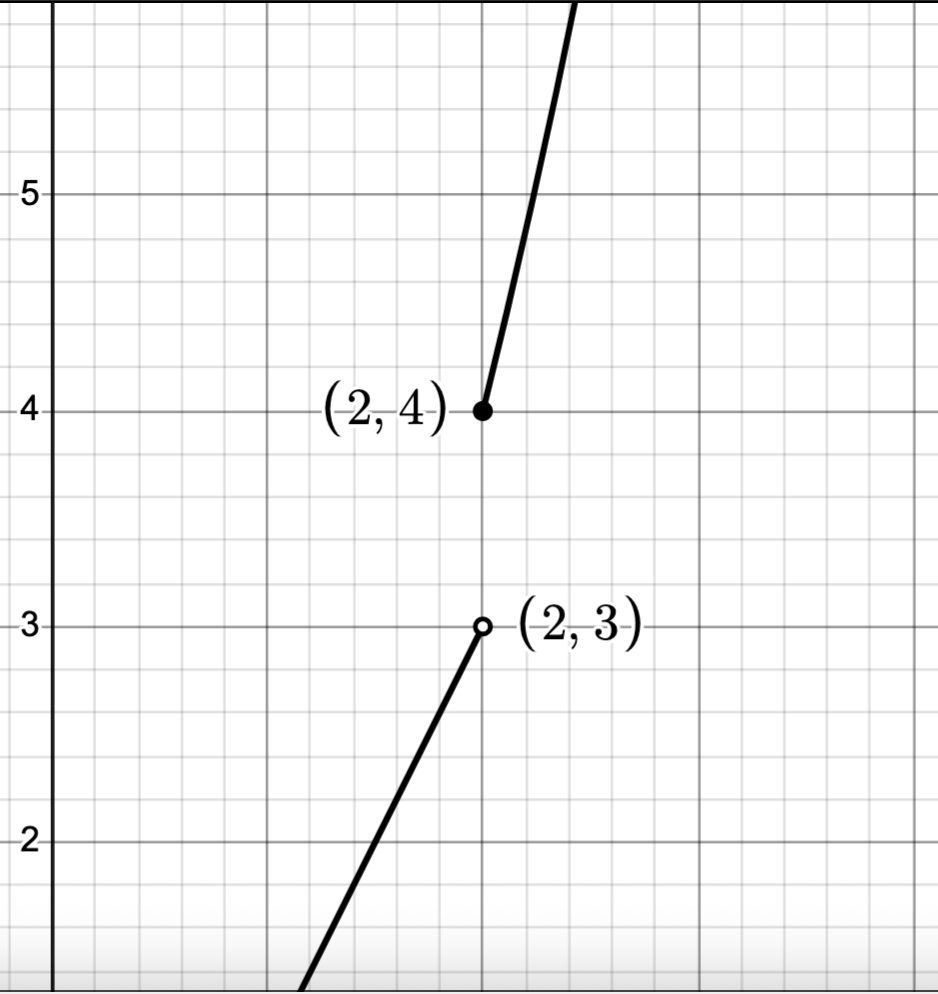
\includegraphics[width=3in]{./IntroLimitsGraphics/jumpdisc.png} &  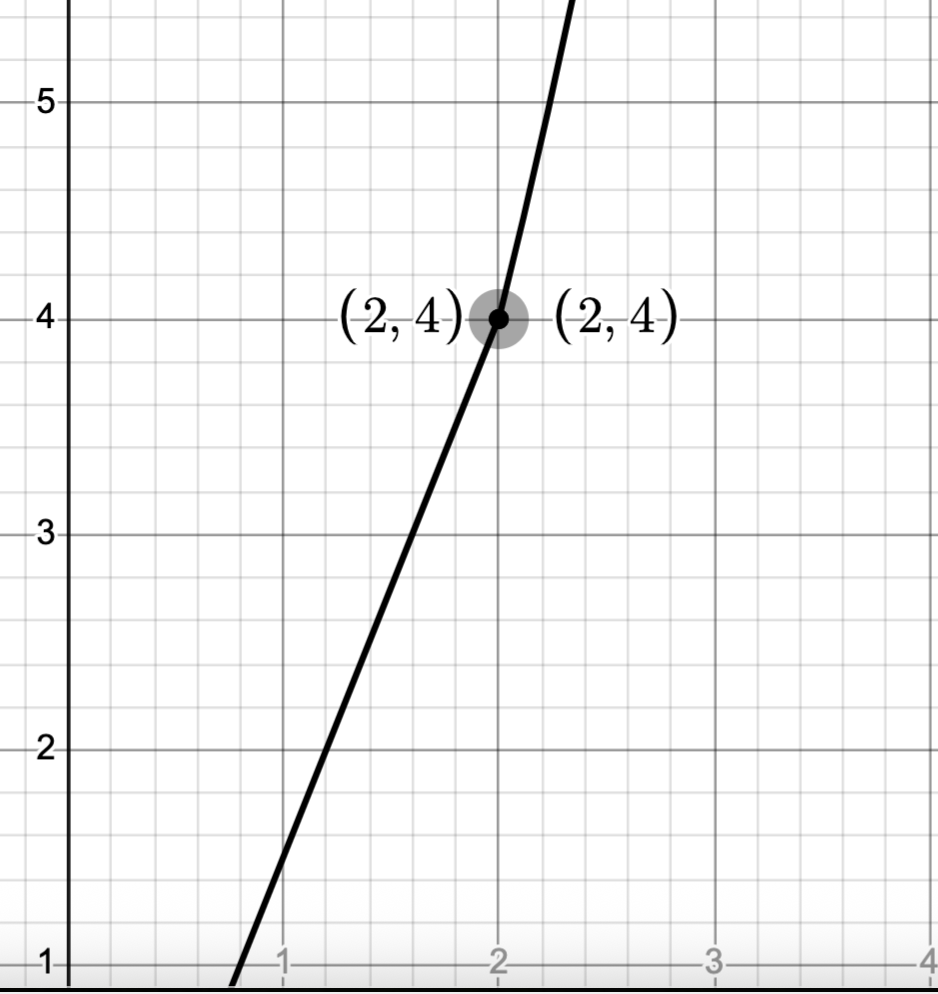
\includegraphics[width=3in]{./IntroLimitsGraphics/glued.png} \\
 
 $y = f(x)$ near $x = 2$ & $y = g(x)$ near $x = 2$  \\
 
 \end{tabular}
 
 \hfill \qed
 
 \end{center}

\end{enumerate}
\end{example}

It is worth noting that despite each `piece' of the piecewise-defined function $f$ in Example \ref{piecewisecontex} being continuous, the pieces don't match up at $x=2$ causing what is called a\index{discontinuity ! jump} \textbf{discontinuity}.   A discontinuity is a place where a function is \textbf{not} continuous.  The particular variety of discontinuity appearing here  is usually called a `jump' discontinuity - a type of discontinuity belonging to a larger class of  `non-removable' or `essential' discontinuities.  We'll point out other types of discontinuities as we encounter them.\footnote{Probably in the footnotes because, after all, this is (supposedly) a \underline{pre}calculus book, not a Calculus book \ldots} 

\medskip

We close this section with an example that ties (most of) the fundamental concepts of limits and their calculations together.

\medskip

\begin{example} \label{rationallimit}  Let  $f(x) =  \frac{x^2-2x-3}{x^2-1}$.  Find $\ds{\lim_{x \rightarrow -1} f(x)}$ analytically\footnote{i.e, using properties of limits} and interpret graphically.

\medskip

{\bf Solution.}  Since $f$ is a rational function, and rational functions are continuous on their domains, it's worth checking to see what happens when we attempt to find $f(-1)$.  We get  $f(-1) = \frac{(-1)^2 - 2(-1)-3}{(-1)^2-1} = \frac{0}{0},$ which is undefined because of the `$0$' in the denominator.  However, the `$0$' in the numerator signals to us\footnote{courtesy of the Factor Theorem (Theorem \ref{factorthm}) \ldots} there are common factors of $(x-(-1)) = (x+1)$ which will cancel and potentially help us determine the indeterminate form.  To that end, we simplify: $f(x) =  \frac{x^2-2x-3}{x^2-1} = \frac{(x-3)(x+1)}{(x-1)(x+1)} = \frac{(x-3)\cancel{(x+1)}}{(x-1)\cancel{(x+1)}} = \frac{x-3}{x-1}, \quad x \neq -1$. 

\medskip

That is, for all real numbers \textbf{except} $x = -1$, $\frac{x^2-2x-3}{x^2-1} = \frac{x-3}{x-1}$.   Since $\ds{\lim_{x \rightarrow -1} f(x)}$ is concerned only with what's happening \textbf{near} $x = -1$, but not with what's happening \textbf{at} $x = -1$, it seems reasonable to suggest that $\ds{\lim_{x \rightarrow -1} f(x) =  \lim_{x \rightarrow -1}}$  $\frac{x^2-2x-3}{x^2-1} =$  $\ds{\lim_{x \rightarrow -1}}$ $\frac{x-3}{x-1}$.

\medskip

Note that $x = -1$ is in the domain of the function $g(x) = \frac{x-3}{x-1}$, hence $g$  \textbf{is} continuous at $x = -1$.   This means $\ds{\lim_{x \rightarrow -1} g(x) = g(-1)}$, that is, $\ds{\lim_{x \rightarrow -1}}$ $\frac{x-3}{x-1} = \frac{-1-3}{-1-1} = 2$.

\medskip

Putting all of this work together, we get $\ds{\lim_{x \rightarrow -1} f(x) =   \lim_{x \rightarrow -1}}$ $ \frac{x-3}{x-1}  =  \frac{-1-3}{-1-1} = 2$.   Graphically, this means there is a hole in the graph of $f$ at the location $(-1,2)$.\footnote{Since $f(-1)$ is undefined but  $\ds{\lim_{x \rightarrow -1} f(x)}$ exists means the discontinuity here is classified as `removable.'  We can `remove' the discontinuity by `patching' the `hole' by defining $f(-1) = 2$. We do such repairs in Calculus.}  The table and graph below confirm our answer.\footnote{Note that depending on which graphing utility is used, the `hole' at $(-1,2)$ may or may not be immediately visible on the graph.}

\begin{center}

 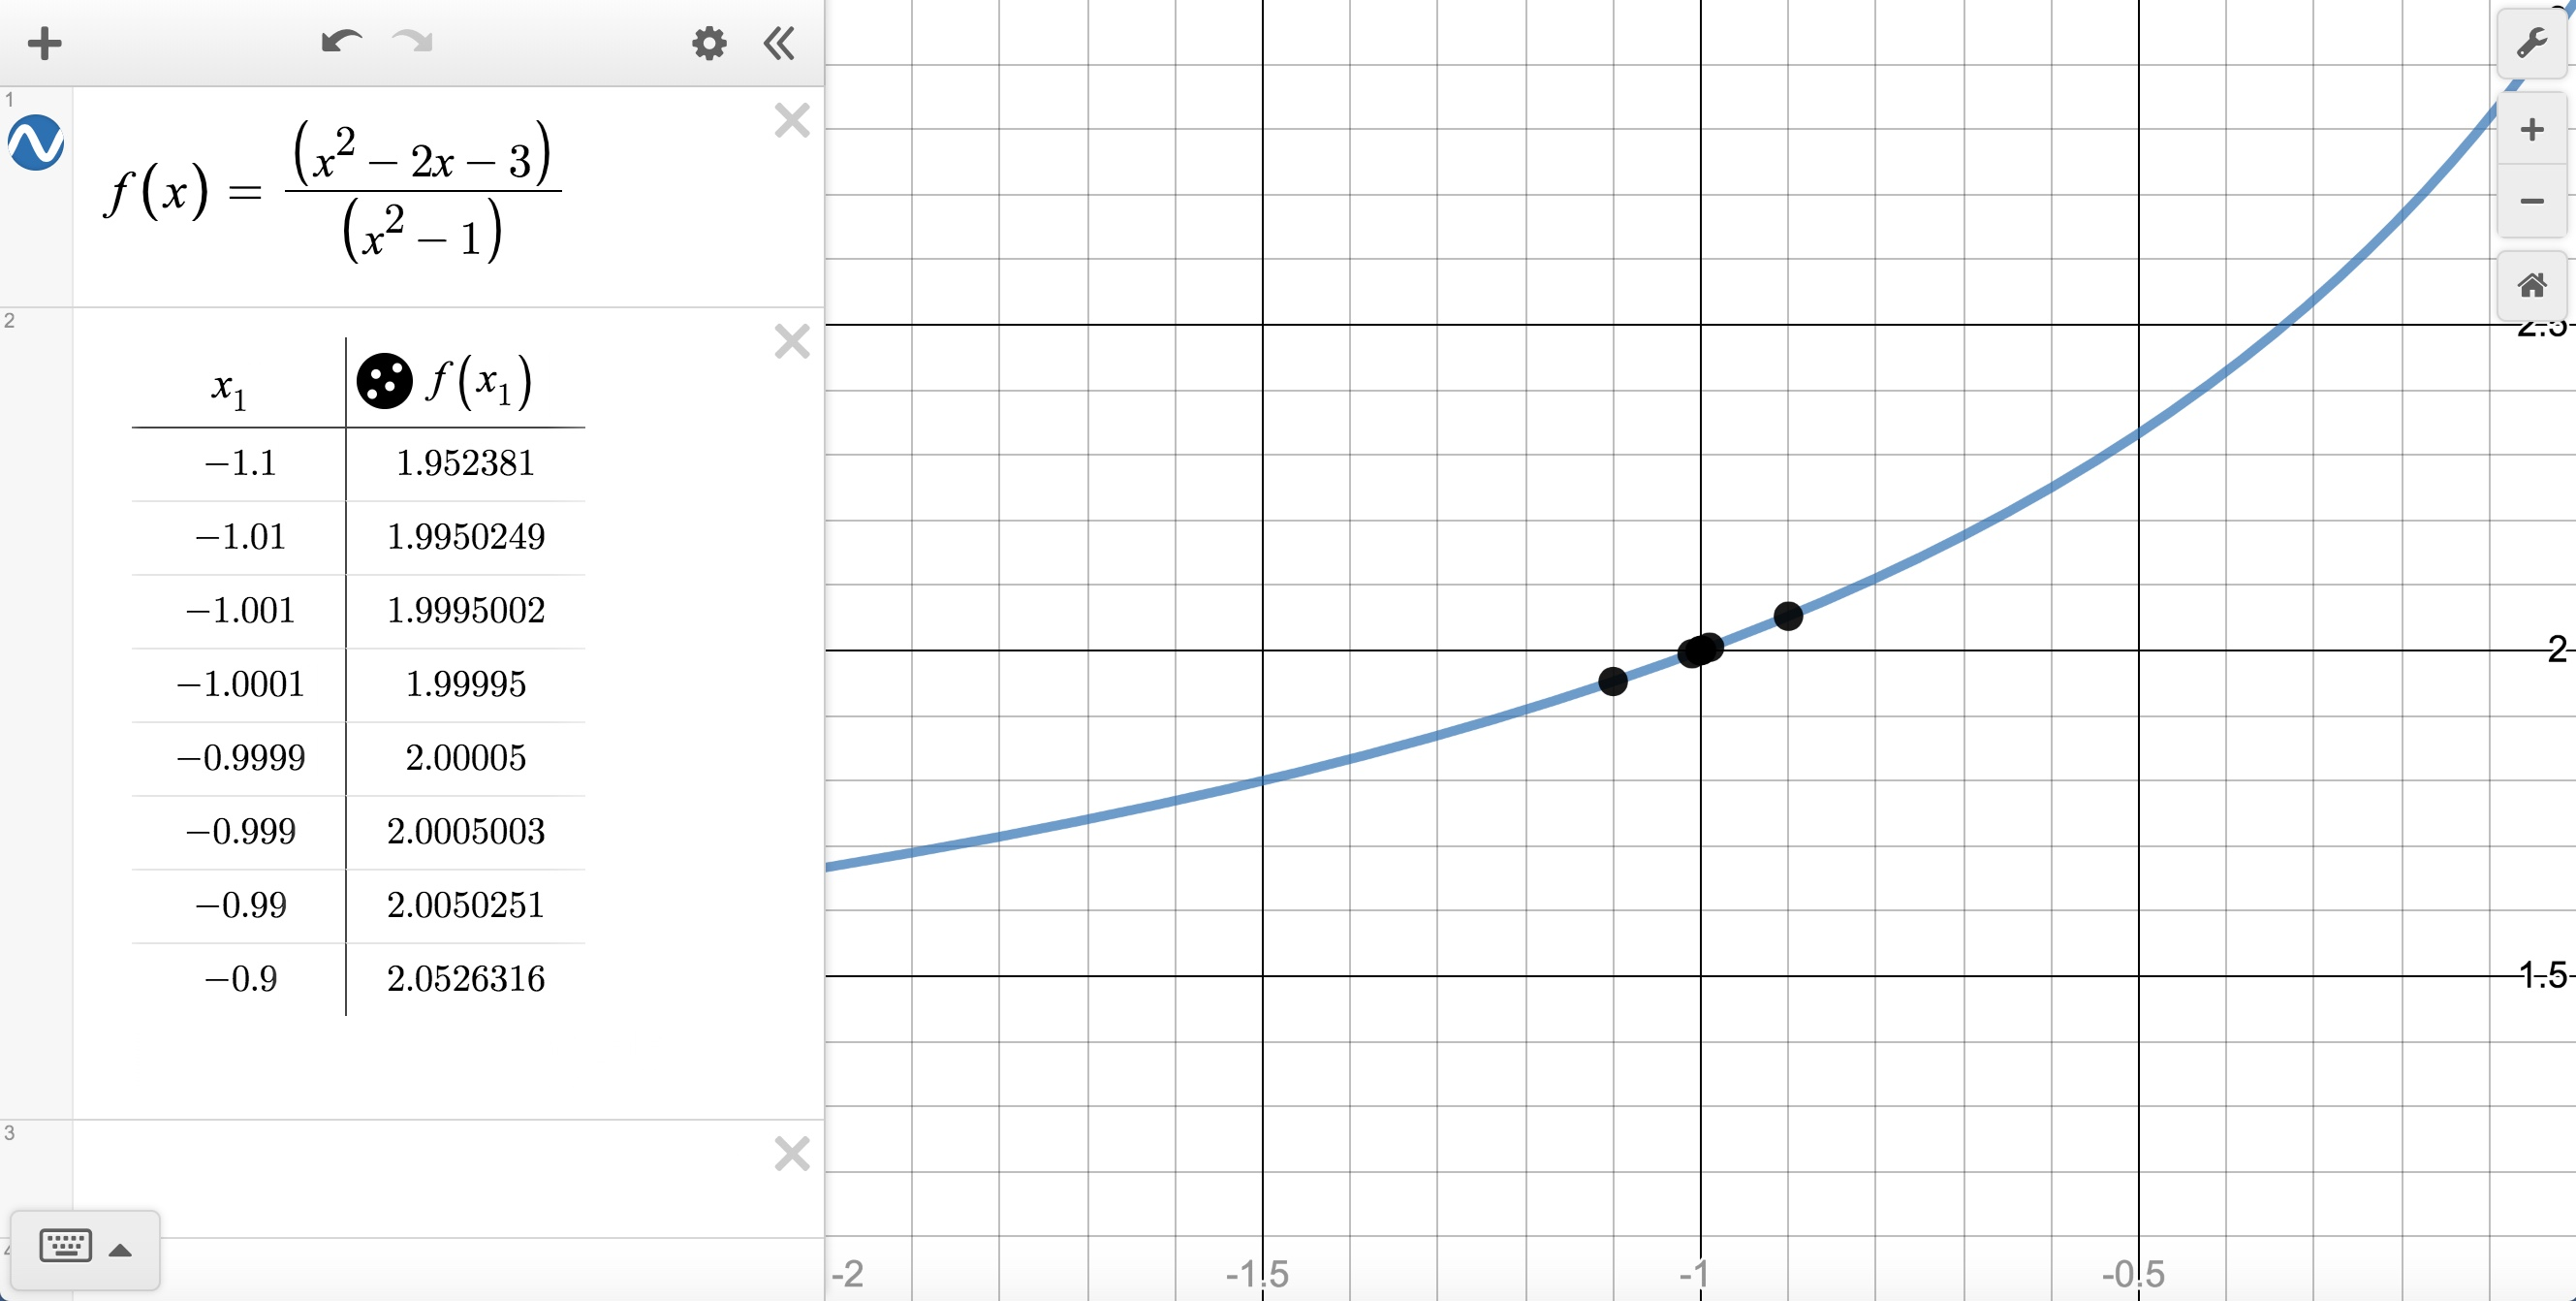
\includegraphics[width=5in]{./IntroLimitsGraphics/NearNegativeOne.jpeg} 
 
 $y = f(x)$ near $x = -1$

\end{center}

\hfill \qed



\end{example}

\medskip

The above reasoning is sound and is true in general.  We'll be getting a lot of use out of the following:

\medskip

%% \colorbox{ResultColor}{\bbm

\begin{theorem}  \label{limitsagree} If $f$ and $g$ are two functions which agree on an open interval containing $x = a$, except possibly at $x = a$, then if $\ds{\lim_{x \rightarrow a} g(x)}$ exists, $\ds{ \lim_{x \rightarrow a} f(x) = \lim_{x \rightarrow a} g(x)}$.


\end{theorem}
%% \ebm}







\newpage

\subsection{Exercises}
%% SKIPPED %% \label{ExercisesforIntroLimits}

\begin{enumerate}

\item  Consider the complete graph of the function $f$ below.  Use the graph to find the indicated values.

\smallskip

If a limit fails to exist, state that is the case  or use the symbols `$\infty$' or `$-\infty$' appropriately.
 
 \smallskip
 
 \textbf{NOTE:}  The graph has a vertical asymptote $x=3$.  

\begin{center}

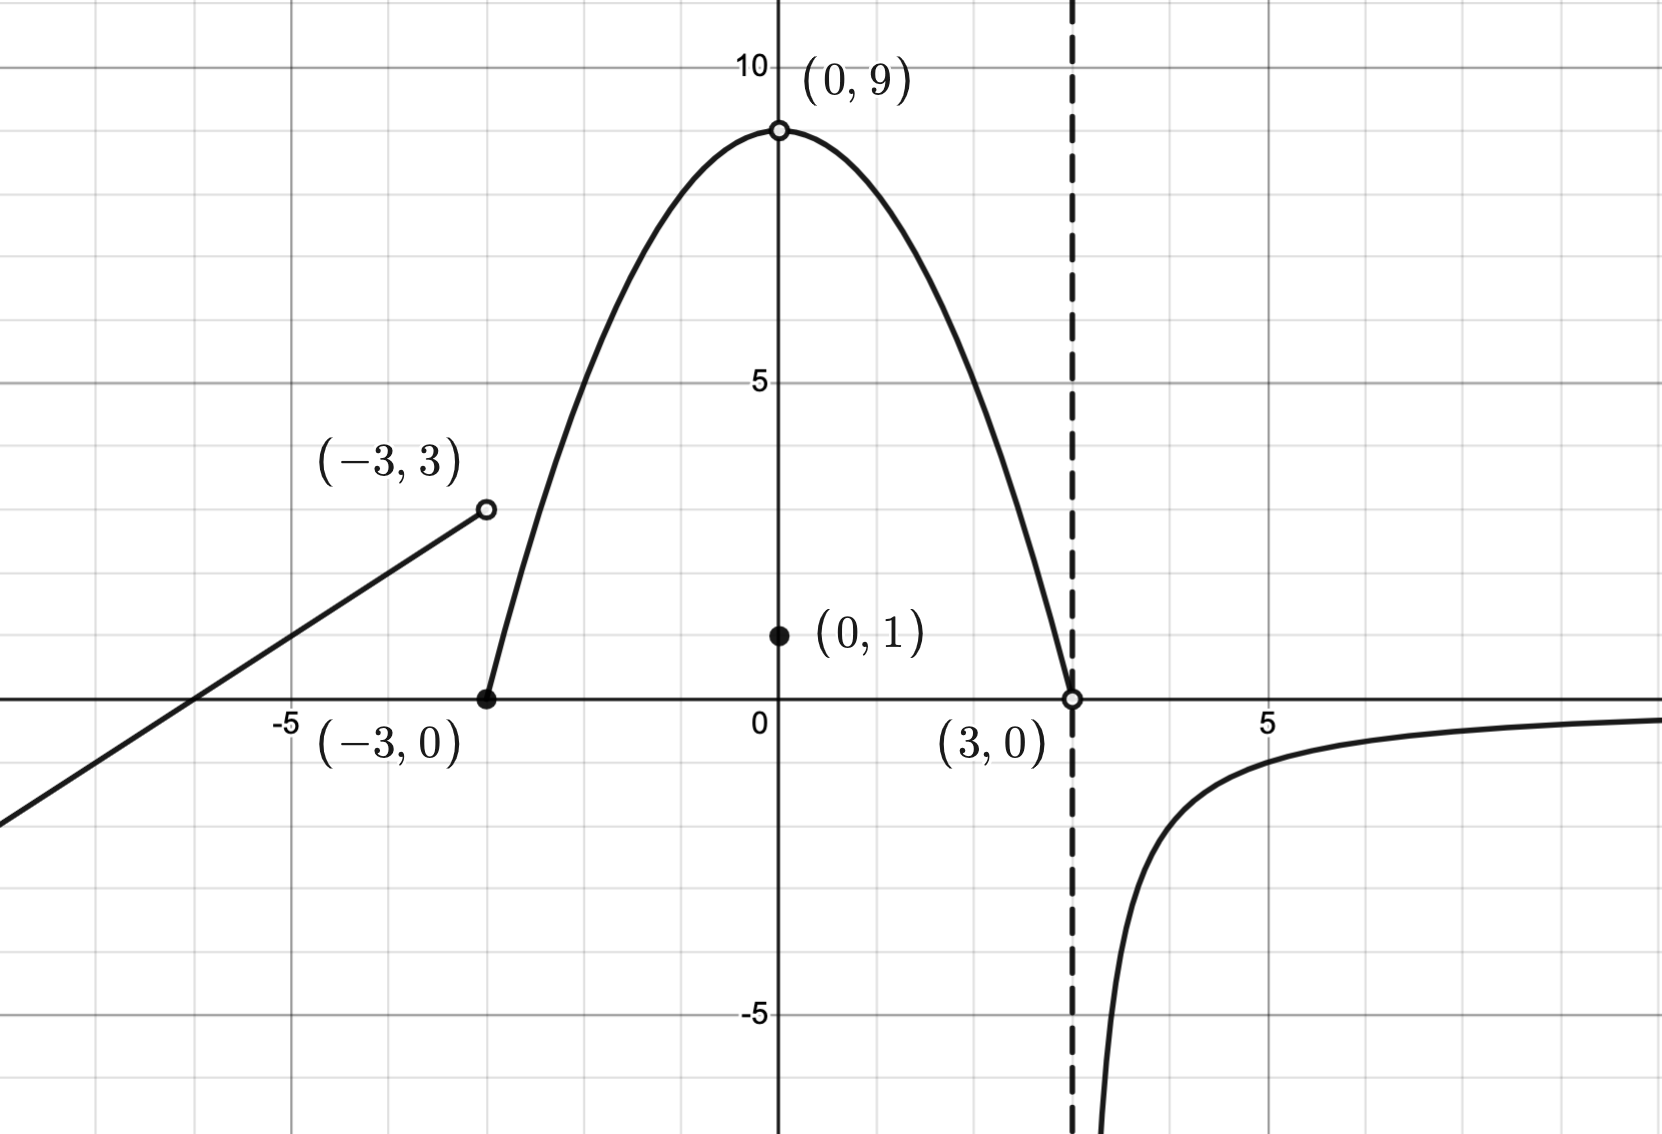
\includegraphics[width=5.5in]{./IntroLimitsGraphics/M2500TH01.png}

\end{center}

\bigskip

\begin{multicols}{4}

\begin{itemize}

\item $\ds{\lim_{x \rightarrow -3^{-}} f(x)}$

\item $\ds{\lim_{x \rightarrow -3^{+}} f(x)}$

\item $\ds{\lim_{x \rightarrow -3} f(x)}$

\item $f(-3)$

\end{itemize}

\end{multicols}

\bigskip

\begin{multicols}{4}

\begin{itemize}

\item $\ds{\lim_{x \rightarrow 0} f(x)}$

\item  $f(0)$

\item $\ds{\lim_{x \rightarrow 3^{-}} f(x)}$

\item $\ds{\lim_{x \rightarrow 3^{+}} f(x)}$
\end{itemize}

\end{multicols}

\bigskip


\item\label{twosidedonesidedlimitexistexercise}  \begin{enumerate}  \item  Explain why if $\ds{\lim_{x \rightarrow a} f(x)}$ exist, then so do $\ds{\lim_{x \rightarrow a^{-}} f(x)}$ and $\ds{\lim_{x \rightarrow a^{+}} f(x)}$.

\item   Find an instance\footnote{There are a few examples to be found in Example \ref{limitfromgraphex} \ldots}  where   $\ds{\lim_{x \rightarrow a^{-}} f(x)}$ and $\ds{\lim_{x \rightarrow a^{+}} f(x)}$ both exist but $\ds{\lim_{x \rightarrow a} f(x)}$ does not.

\end{enumerate}

\item  Consider the complete graph of the function $g$ below.  Use the graph to find the indicated values.

\smallskip


If a limit fails to exist, state that is the case  or use the symbols `$\infty$' or `$-\infty$' appropriately.
  
\smallskip

 
 \textbf{NOTE:}  The graph has a vertical asymptote $x=-2$ and a horizontal asymptote $y = 1$.  



\begin{center}

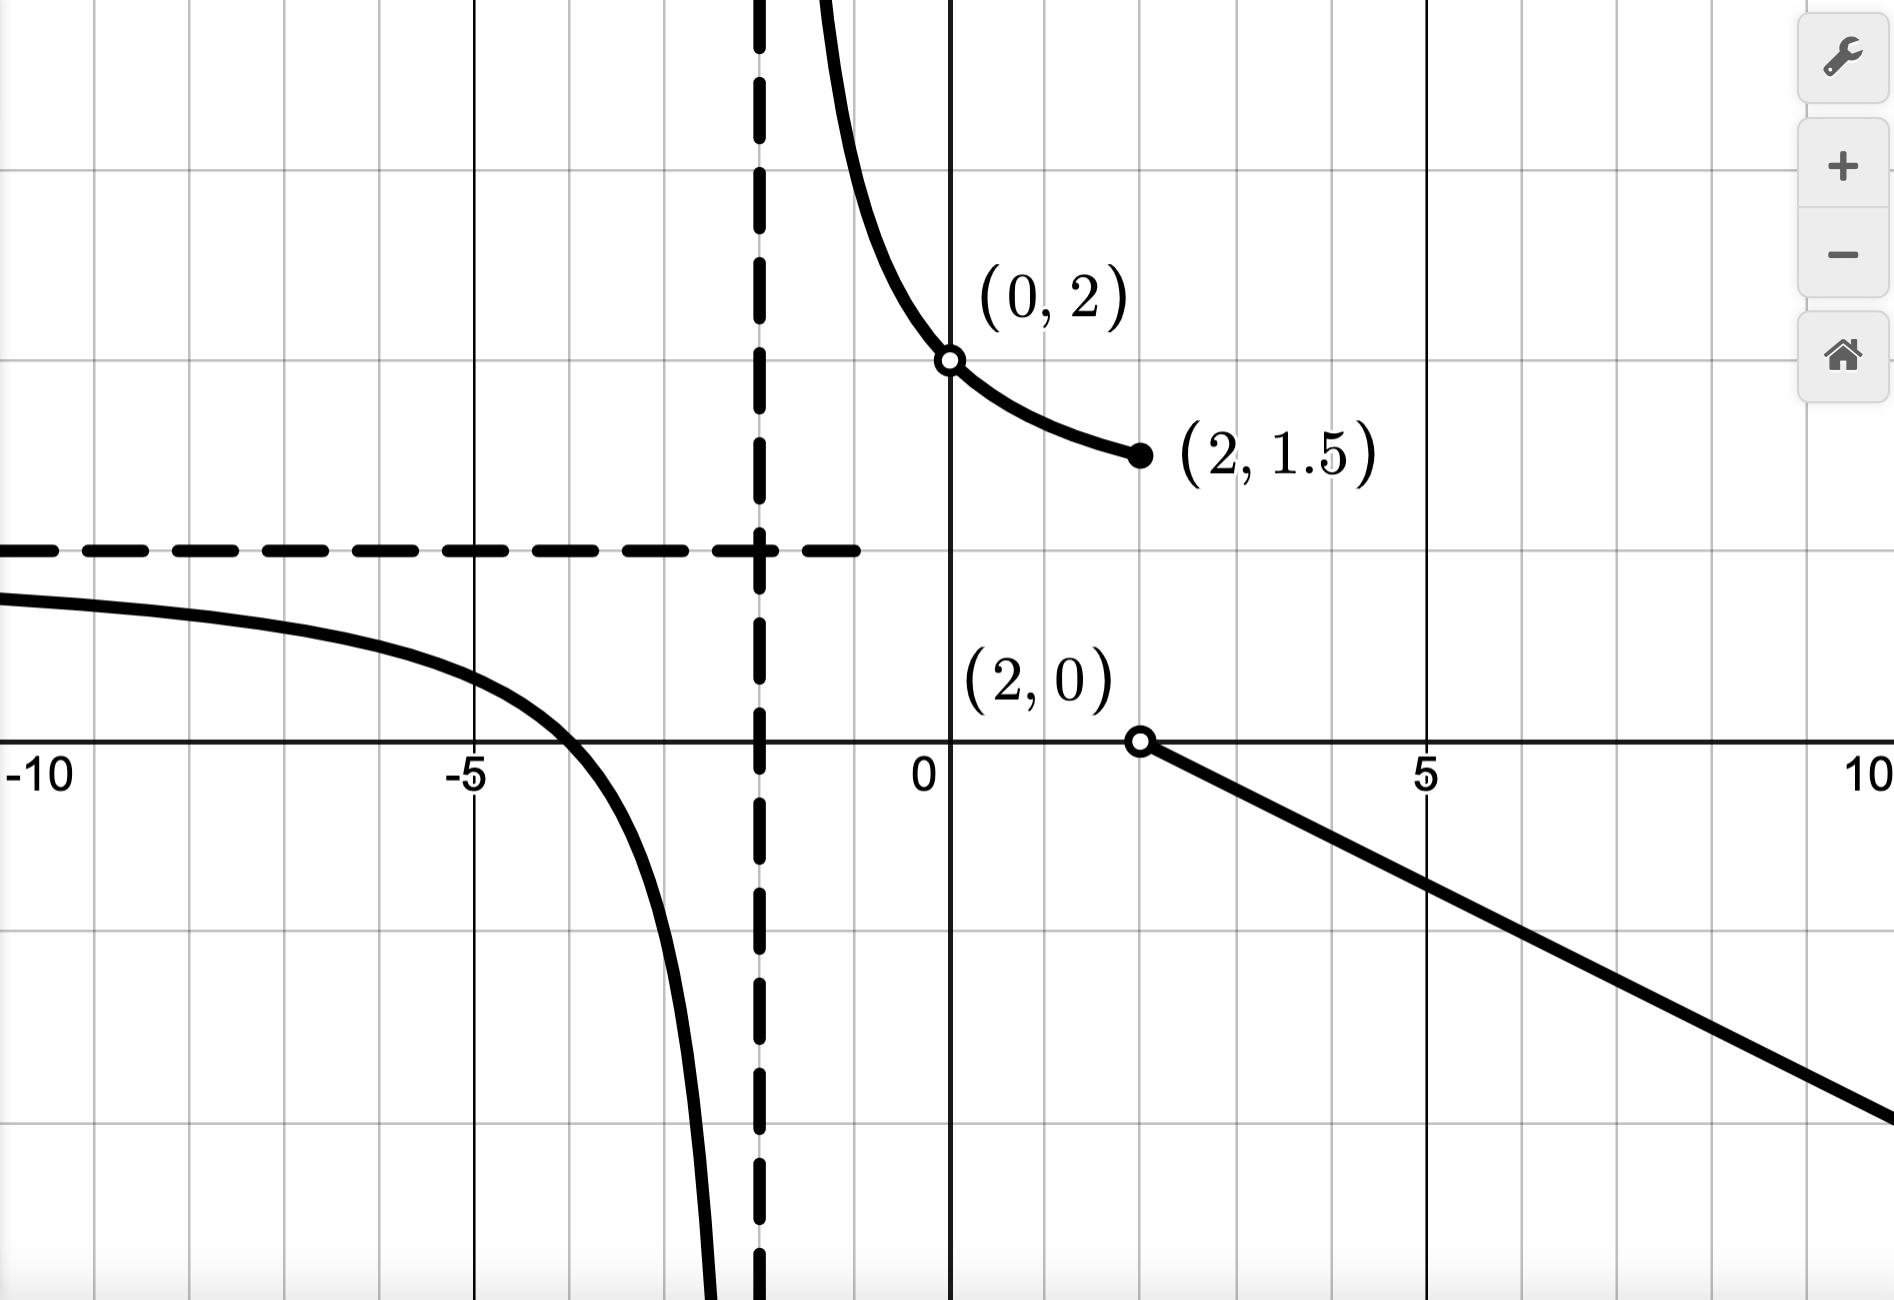
\includegraphics[width=5.5in]{./IntroLimitsGraphics/M2500_T01_Sp25_a.png}

\end{center}

\bigskip

\begin{multicols}{4}

\begin{itemize}

\item $\ds{\lim_{x \rightarrow -\infty} g(x)}$

\item $\ds{\lim_{x \rightarrow -2^{-}} g(x)}$

\item $\ds{\lim_{x \rightarrow -2^{+}} g(x)}$

\item  $\ds{\lim_{x \rightarrow \infty} g(x)}$

\end{itemize}

\end{multicols}

\bigskip

\begin{multicols}{4}

\begin{itemize}

\item $\ds{\lim_{x \rightarrow 0} g(x)}$

\item $\ds{\lim_{x \rightarrow 2^{-}} g(x)}$

\item  $g(2)$

\item $\ds{\lim_{x \rightarrow 2^{+}} g(x)}$
\end{itemize}

\end{multicols}

\bigskip

\setcounter{HW}{\value{enumi}}
\end{enumerate}

For Exercises \ref{factorcancelfirst} - \ref{factorcancellast}, find the limit analytically using Exercise \ref{rationallimit} as a guide.  If a limit fails to exist, state that is the case  or use the symbols `$\infty$' or `$-\infty$' appropriately.
 
\begin{multicols}{3}

\begin{enumerate}
\setcounter{enumi}{\value{HW}}

\item\label{factorcancelfirst}  $\ds{\lim_{x \rightarrow 2} \dfrac{2x^2+x-3}{x^2-1}}$
  
\item  $\ds{\lim_{x \rightarrow 1} \dfrac{2x^2+x-3}{x^2-1}}$

\item   $\ds{\lim_{x \rightarrow -1} \dfrac{2x^2+x-3}{x^2-1}}$

\setcounter{HW}{\value{enumi}}
\end{enumerate}

\end{multicols}

\begin{multicols}{3}

\begin{enumerate}
\setcounter{enumi}{\value{HW}}

\item   $\ds{\lim_{x \rightarrow -1^{+}} \dfrac{2x^2+x-3}{x^2-1}}$

\item  $\ds{\lim_{x \rightarrow 3} \dfrac{x^2-3x}{x^2-x-6}}$

\item\label{factorcancellast}  $\ds{\lim_{x \rightarrow 3} \dfrac{x^2-6x}{x^2-6x+9}}$

\setcounter{HW}{\value{enumi}}
\end{enumerate}

\end{multicols}

For Exercises \ref{abscancelfirst} - \ref{abscancellast}, use the piecewise definition of absolute value, Definition \ref{absolutevaluepiecewise} to help you find the limit analytically.    If a limit fails to exist, state that is the case  or use the symbols `$\infty$' or `$-\infty$' appropriately.

\begin{multicols}{2}
\begin{enumerate}
\setcounter{enumi}{\value{HW}}

\item\label{abscancelfirst} $\ds{ \lim_{x \rightarrow 3^{-}} \dfrac{|3x - x^2| }{x-3}}$     

\item\label{abscancellast}  $\ds{\lim_{x \rightarrow 2^{+}} \dfrac{|6-3x|}{x^2-4x+4}}$

\setcounter{HW}{\value{enumi}}
\end{enumerate}
\end{multicols}

For Exercises \ref{complexcancelfirst} - \ref{complexcancellast}, simplify the complex fraction in order to help you find the limit analytically.\footnote{A review of Section \ref{AppRatExpEqus} may be in order.}  If a limit fails to exist, state that is the case  or use the symbols `$\infty$' or `$-\infty$' appropriately.

\begin{multicols}{3}
\begin{enumerate}
\setcounter{enumi}{\value{HW}}

\item\label{complexcancelfirst}  $\ds{\lim_{x \rightarrow 1} \dfrac{\dfrac{x}{x-2} +1}{x-1}}$

\item $\ds{ \lim_{x \rightarrow 2} \dfrac{\dfrac{2x}{x+2}  -1}{x-2} }$ 
     
\item\label{complexcancellast} $\ds{ \lim_{h \rightarrow 0} \dfrac{\dfrac{1}{2(x+h) - 1}  - \dfrac{1}{2x-1} }{h} }$ 

\setcounter{HW}{\value{enumi}}
\end{enumerate}
\end{multicols}

For Exercises \ref{radicalcancelfirst} - \ref{radicalcancellast}, rationalize the numerator of the fraction in order to help you find the limit analytically.\footnote{A review of Section \ref{rationalizingdenomandnumer} may be in order.} If a limit fails to exist, state that is the case  or use the symbols `$\infty$' or `$-\infty$' appropriately.


\begin{multicols}{3}
\begin{enumerate}
\setcounter{enumi}{\value{HW}}

 \item\label{radicalcancelfirst}  $\ds{ \lim_{x \rightarrow -1} \dfrac{\sqrt{x+5} - 2 }{x+1} }$  
   
 \item   $\ds{\lim_{h \rightarrow 0} \dfrac{\sqrt{4+h} - 2}{h}}$

\item\label{radicalcancellast} $\ds{ \lim_{h \rightarrow 0} \dfrac{\sqrt{2x+2h-1} - \sqrt{2x-1} }{h} }$  

\setcounter{HW}{\value{enumi}}
\end{enumerate}
\end{multicols}


 In Exercises \ref{limitatinfinityfirst} - \ref{limitatinfinitylast},  find the limit analytically.  Use the symbols `$\infty$' and `$-\infty$' as appropriate.

 \begin{multicols}{3}
\begin{enumerate}
\setcounter{enumi}{\value{HW}}

\item\label{limitatinfinityfirst}   $\ds{ \lim_{x \rightarrow \infty} \dfrac{3x-4}{2x+1}}$

\item $\ds{ \lim_{x \rightarrow -\infty}  \dfrac{1-2x}{x-5}}$ 

\item $\ds{ \lim_{x \rightarrow -\infty}\dfrac{2x-1}{x^2+4}}$

\setcounter{HW}{\value{enumi}}
\end{enumerate}
\end{multicols}

 \begin{multicols}{3}
\begin{enumerate}
\setcounter{enumi}{\value{HW}}
\item $\ds{ \lim_{x \rightarrow \infty}\dfrac{\sqrt{4x^2+x-1}}{1-x}}$

\item $\ds{ \lim_{x \rightarrow -\infty}\dfrac{\sqrt{4x^2+x-1}}{1-x}}$

\item\label{limitatinfinitylast}  $\ds{ \lim_{x \rightarrow \infty} \dfrac{x^2+2x+3}{4-x}}$.

\setcounter{HW}{\value{enumi}}
\end{enumerate}
\end{multicols}

\begin{enumerate}
\setcounter{enumi}{\value{HW}}

\item  Let $f(x) = \dfrac{x}{\lfloor x \rfloor}$  where `$\lfloor x \rfloor$'  is the greatest integer (or floor) function.\footnote{See Example \ref{greatestintegerdefn} in Section \ref{ConstantandLinearFunctions} for review, if needed.} 

\smallskip

Fill in the blanks below to help you analyze $\ds{ \lim_{x \rightarrow 0} f(x)}$.

\smallskip

\begin{enumerate}

\item  If $-1 < x < 0$, then $\lfloor x \rfloor = \underline{\hspace{1in}}$. So we can rewrite $f(x) = \dfrac{x}{\lfloor x \rfloor} =  \underline{\hspace{1in}}$.

\item  Using part (a), we can find  $\ds{ \lim_{x \rightarrow 0^{-}} f(x) =  \lim_{x \rightarrow 0^{-}}  \underline{\hspace{1in}} =  \underline{\hspace{1in}} }$.

\item  If $0 < x < 1$, then $\lfloor x \rfloor = \underline{\hspace{1in}}$, hence $f(x) = \dfrac{x}{\lfloor x \rfloor}$ does not exist as $x \rightarrow 0^{+}$.

\item  Putting parts (b) and (c) together, we have that   $\ds{ \lim_{x \rightarrow 0} f(x)  \qquad \underline{\hspace{1.5in}}}$

\item  Graph $f(x) = \dfrac{x}{\lfloor x \rfloor}$ on desmos near $x = 0$ to confirm your answers.

\end{enumerate}

\newpage

\item  Sketch the graph of a function which satisfies all of the following criteria:

\bigskip

\begin{multicols}{4}

\begin{itemize}

\item $\ds{\lim_{x \rightarrow -\infty}  f(x) = \infty}$

\item $\ds{\lim_{x \rightarrow 4^{-}} f(x) = 6}$

\item $\ds{\lim_{x \rightarrow 4^{+}} f(x) = - \infty}$

\item $\ds{\lim_{x \rightarrow \infty}  f(x) =0}$

\end{itemize}

\end{multicols}

\item Sketch the graph of a function $f$  which satisfies all of the following criteria:

\bigskip

\begin{multicols}{3}

\begin{itemize}

\item $\ds{\lim_{x \rightarrow -\infty} f(x) = 2}$

\item $\ds{\lim_{x \rightarrow 0^{-}} f(x) = \infty}$

\item $\ds{\lim_{x \rightarrow 0^{+}} f(x) = -\infty}$

\end{itemize}

\end{multicols}

\bigskip

\begin{multicols}{3}

\begin{itemize}

\item $\ds{\lim_{x \rightarrow 2^{-}} f(x) = 3}$

\item $\ds{\lim_{x \rightarrow 2^{+}} f(x) =0}$

\item $\ds{\lim_{x \rightarrow \infty} f(x) = -\infty}$

\end{itemize}

\end{multicols}


\item\label{onesidedcontinuityexercise}  A function is said to be \index{continuous from the left}\index{continuous ! from the left}\index{one-sided continuity}\index{continuity ! one sided}\textbf{continuous from the left} at $x=a$ if $\ds{\lim_{x \rightarrow a^{-}} f(x) = f(a)}$.  Likewise, a function is said to be \index{continuous from the right}\index{continuous ! from the right}\index{one-sided continuity}\index{continuity ! one sided}\textbf{continuous from the right} at $x=a$ if $\ds{\lim_{x \rightarrow a^{+}} f(x) = f(a)}$.

\begin{enumerate}

\item   Explain why $r(x) = \sqrt{5-x}$ is not continuous at $x = 5$.  Is $r$ continuous from the left at $x=5$?  From the right?  Explain.

\item  Explain why the floor function\footnote{See Example \ref{greatestintegerdefn} in Section \ref{ConstantandLinearFunctions} for review, if needed.} $F(x) = \lfloor x \rfloor$ is not continuous at $x = 117$.   Is $F$ continuous from the left at $x=117$?  From the right?  Explain.

\item  If a function $f$ is continuous at $x = a$, explain why $f$ is continuous from both the left and the right at $x = a$.  Is the converse true?  That is, if $f$ is continuous from both the left and the right at $x = a$, is $f$ continuous at $x=a$?  

\item  Compare and contrast your answers in this exercise to those in Exercise \ref{twosidedonesidedlimitexistexercise}.


\end{enumerate}


\item  Consider the table of values below:

\[ \begin{array}{|r|c|} 

\hline

x & f(x)  \\    \hline 

-0.001  &  1.9 \\   [1ex]  \hline 

-0.0001 & 1.99 \\ [1ex]  \hline

-0.00001 & 1.999\\  [1ex] \hline

-0.000001 & 1.9999 \\ [1ex]  \hline

0.000001 & -10000\\  [1ex]   \hline

0.00001 & -1000 \\ [1ex]  \hline

0.0001 & - 100 \\  [1ex] \hline

0.001 & -10 \\ [1ex]  \hline


\end{array} \]

It turns out that $\ds{\lim_{x \rightarrow 0} f(x) = 117}$.  How is this possible assuming the data in the table is correct?

\item  In this exercise, we use Definition \ref{infinitelimitsatinfinity} to prove $\ds{\lim_{x \rightarrow \infty} x^3 = \infty}$ and $\ds{\lim_{x \rightarrow -\infty} x^3 = -\infty}$:


\begin{enumerate}

\item  Solve the following inequalities:

\begin{multicols}{4}

\begin{itemize}

\item  $x^3 > 1000$

\item  $x^3 > 100000$

\item  $x^3 > 10^{99}$

\item  $x^3 > N$

\end{itemize}

\end{multicols}

\item  Show that for $N > 0$, if $x > \sqrt[3]{N}$, then $x^3 > N$.  Write a sentence (or two!) which uses your work and Definition \ref{infinitelimitsatinfinity} to prove $\ds{\lim_{x \rightarrow \infty} x^3 = \infty}$.

\item  Repeat a similar argument to prove $\ds{\lim_{x \rightarrow -\infty} x^3 = -\infty}$

\end{enumerate}
 
\end{enumerate}

\newpage

\subsection{Answers}

\begin{enumerate}

\item  \begin{multicols}{4} \begin{itemize} \item $\ds{\lim_{x \rightarrow -3^{-}} f(x) = 3}$

\item $\ds{\lim_{x \rightarrow -3^{+}} f(x) = 0}$

\item $\ds{\lim_{x \rightarrow -3} f(x)}$ d.n.e.

\item $f(-3) = 0$

\end{itemize}

\end{multicols}

\bigskip

\begin{multicols}{4}

\begin{itemize}

\item $\ds{\lim_{x \rightarrow 0} f(x) = 9}$

\item  $f(0)$

\item $\ds{\lim_{x \rightarrow 3^{-}} f(x) = 0}$

\item $\ds{\lim_{x \rightarrow 3^{+}} f(x) = -\infty}$
\end{itemize}

\end{multicols}

\bigskip


\item  \begin{enumerate}  \item  If $\ds{\lim_{x \rightarrow a} f(x)}$ exists, say $\ds{\lim_{x \rightarrow a} f(x) = L}$ then the $f(x)$ values approach  $L$  as $x \rightarrow a$ from both directions.  Hence both one-sided limits exist.  In particular,  $\ds{\lim_{x \rightarrow a^{-}} f(x) = L}$ and $\ds{\lim_{x \rightarrow a^{+}} f(x) = L}$.

\item  In Example \ref{limitfromgraphex},  $\ds{\lim_{x \rightarrow -1^{-}} f(x)  = 0}$ and $\ds{\lim_{x \rightarrow -1^{+}} f(x) = 4}$ both exist but $\ds{\lim_{x \rightarrow -1} f(x)}$ does not because the two one-sided limits are not equal.

\end{enumerate}

\item  \begin{multicols}{4} \begin{itemize} \item $\ds{\lim_{x \rightarrow -\infty} g(x) = 1}$

\item $\ds{\lim_{x \rightarrow -2^{-}} g(x) = -\infty}$

\item $\ds{\lim_{x \rightarrow -2^{+}} g(x) = \infty}$

\item  $\ds{\lim_{x \rightarrow \infty} g(x) = -\infty}$

\end{itemize}

\end{multicols}

\bigskip

\begin{multicols}{4}

\begin{itemize}

\item $\ds{\lim_{x \rightarrow 0} g(x) = 2}$

\item $\ds{\lim_{x \rightarrow 2^{-}} g(x) = 1.5}$

\item  $g(2) = 1.5$

\item $\ds{\lim_{x \rightarrow 2^{+}} g(x) = 0}$
\end{itemize}

\end{multicols}

\bigskip

\setcounter{HW}{\value{enumi}}
\end{enumerate}
 


\begin{enumerate}
\setcounter{enumi}{\value{HW}}

\item  $\ds{\lim_{x \rightarrow 2} \dfrac{2x^2+x-3}{x^2-1} = \frac{7}{3}}$

\medskip
  
\item  $\ds{\lim_{x \rightarrow 1} \dfrac{2x^2+x-3}{x^2-1} = \frac{5}{2}}$

\medskip

\item   $\ds{\lim_{x \rightarrow -1} \dfrac{2x^2+x-3}{x^2-1}}$ does not exist

\medskip

\setcounter{HW}{\value{enumi}}
\end{enumerate}



\begin{enumerate}
\setcounter{enumi}{\value{HW}}

\item   $\ds{\lim_{x \rightarrow -1^{+}} \dfrac{2x^2+x-3}{x^2-1} = \infty}$

\medskip

\item  $\ds{\lim_{x \rightarrow 3} \dfrac{x^2-3x}{x^2-x-6} = \frac{3}{5}}$


\medskip

\item  $\ds{\lim_{x \rightarrow 3} \dfrac{x^2-6x}{x^2-6x+9} = -\infty}$

\medskip

\setcounter{HW}{\value{enumi}}
\end{enumerate}




\begin{enumerate}
\setcounter{enumi}{\value{HW}}

\item  $\ds{ \lim_{x \rightarrow 3^{-}} \dfrac{|3x - x^2| }{x-3} = -3}$ 

\medskip    

\item $\ds{\lim_{x \rightarrow 2} \dfrac{|6-3x|}{x^2-4x+4} = \infty}$

\medskip

\setcounter{HW}{\value{enumi}}
\end{enumerate}

\begin{enumerate}
\setcounter{enumi}{\value{HW}}

\item  $\ds{\lim_{x \rightarrow 1} \dfrac{\dfrac{x}{x-2} +1}{x-1} = -2}$

\medskip

\item $\ds{ \lim_{x \rightarrow 2} \dfrac{\dfrac{2x}{x+2}  -1}{x-2}  = \frac{1}{4}}$ 

\medskip
     
\item $\ds{ \lim_{h \rightarrow 0} \dfrac{\dfrac{1}{2(x+h) - 1}  - \dfrac{1}{2x-1} }{h} = -\frac{2}{(2x-1)^2} }$ 

\medskip

\setcounter{HW}{\value{enumi}}
\end{enumerate}

\begin{enumerate}
\setcounter{enumi}{\value{HW}}

 \item  $\ds{ \lim_{x \rightarrow -1} \dfrac{\sqrt{x+5} - 2 }{x+1}  = \frac{1}{4}}$  
 
 \medskip
 
 \item $\ds{\lim_{h \rightarrow 0} \dfrac{\sqrt{4+h} - 2}{h}} = \frac{1}{4}$
 
 \medskip
   
 \item  $\ds{ \lim_{h \rightarrow 0} \dfrac{\sqrt{2x+2h-1} - \sqrt{2x-1} }{h}  = \frac{1}{\sqrt{2x-1}}}$  

\medskip

\setcounter{HW}{\value{enumi}}
\end{enumerate}

\begin{enumerate}
\setcounter{enumi}{\value{HW}}

\item  $\ds{ \lim_{x \rightarrow \infty} \dfrac{3x-4}{2x+1} = \frac{3}{2}}$

\medskip

\item $\ds{ \lim_{x \rightarrow -\infty}  \dfrac{1-2x}{x-5} = -2}$ 

\medskip

\item $\ds{ \lim_{x \rightarrow -\infty}\dfrac{2x-1}{x^2+4} = 0}$

\medskip

\setcounter{HW}{\value{enumi}}
\end{enumerate}

\begin{enumerate}
\setcounter{enumi}{\value{HW}}
\item $\ds{ \lim_{x \rightarrow \infty}\dfrac{\sqrt{4x^2+x-1}}{1-x} = -2}$

\medskip

\item $\ds{ \lim_{x \rightarrow -\infty}\dfrac{\sqrt{4x^2+x-1}}{1-x}  = 2}$

\medskip

\item $\ds{ \lim_{x \rightarrow \infty} \dfrac{x^2+2x+3}{4-x} = -\infty}$

\medskip

\setcounter{HW}{\value{enumi}}
\end{enumerate}


\begin{enumerate}
\setcounter{enumi}{\value{HW}}

\item   \begin{enumerate}

\item  If $-1 < x < 0$, then $\lfloor x \rfloor = -1$. So we can rewrite $f(x) = \dfrac{x}{\lfloor x \rfloor} = -x$.

\smallskip

\item  Using part (a), we can find  $\ds{ \lim_{x \rightarrow 0^{-}} f(x) =  \lim_{x \rightarrow 0^{-}} -x = 0}$.

\smallskip

\item  If $0 < x < 1$, then $\lfloor x \rfloor =0$, hence $f(x) = \dfrac{x}{\lfloor x \rfloor}$ does not exist as $x \rightarrow 0^{+}$.

\smallskip

\item  Putting parts (b) and (c) together, we have that   $\ds{ \lim_{x \rightarrow 0} f(x)}$   does not exist.

\smallskip

\end{enumerate}

\item Answers vary.

\item  Answers vary.

\item \begin{enumerate} \item    The function $r(x) = \sqrt{5-x}$ is not continuous at $x = 5$ since $r$ is undefined if $x>5$, so $\ds{\lim_{x \rightarrow 5^{+}} r(x)}$ does not exist. However, $r$ is continuous from the left at $x = 5$ since 

$\ds{\lim_{x \rightarrow 5^{-}} r(x) =  \lim_{x \rightarrow 5^{-}} \sqrt{5-x} = 0 = \sqrt{5-5} = r(5)}$.

\smallskip

\item  The function  $F(x) = \lfloor x \rfloor$ is not continuous at $x = 117$ since $\ds{\lim_{x \rightarrow 117^{-}} \lfloor x \rfloor = 116}$ but $\ds{\lim_{x \rightarrow 117^{+}} \lfloor x \rfloor = 117}$.  However, $F$ is continuous from the right at $x = 117$ since $\ds{\lim_{x \rightarrow 117^{+}} \lfloor x \rfloor = 117 = \lfloor 117 \rfloor = F(117)}$. 

\smallskip

\item If $f$ is continuous at $x=a$, then $\ds{\lim_{x \rightarrow a} f(x) = f(a)}$.  This means  $\ds{\lim_{x \rightarrow a^{-}} f(x) = f(a)}$ and  $\ds{\lim_{x \rightarrow a^{+}} f(x) = f(a)}$, so $f$ is continuous from both directions at $x=a$. The converse is also true since  ff $\ds{\lim_{x \rightarrow a^{-}} f(x) = f(a)}$ and  $\ds{\lim_{x \rightarrow a^{+}} f(x) = f(a)}$, then $\ds{\lim_{x \rightarrow a} f(x) = f(a)}$.

\smallskip

\item  The difference between the scenario here and that in Exercise \ref{twosidedonesidedlimitexistexercise} is that here, we know what each of the one-sided limits are: $f(a)$. They can't be different numbers like they could be in  Example \ref{limitfromgraphex}

\smallskip

\end{enumerate}


\item  We are told nothing of the function on the interval $(-0.000001, 0.000001 )$ so the function has plenty of opportunities to approach $117$.  


\item \begin{enumerate}

\item \begin{itemize} \item  $x^3 > 1000$ for $x > 10$.

\item  $x^3 > 1000000$ for $x > 100$.

\item  $x^3 > 10^{99}$ for $x > 10^{33}$.

\item  $x^3 > N$ for $x > \sqrt[3]{N}$.

\end{itemize}


\item If $x > \sqrt[3]{N}$, then $x^3 > \left(\sqrt[3]{N} \right)^3 = N$.  Per  Definition \ref{infinitelimitsatinfinity}, given $N>0$, choose $M = \sqrt[3]{N}$.  If $x > M$, then $x^3 > M^3 = N$. Hence,  $\ds{\lim_{x \rightarrow \infty} x^3 = \infty}$.

\smallskip

\item Given $N<0$, choose $M = \sqrt[3]{N}$.  If $x< M$, then $x^3 < M^3 = \left(\sqrt[3]{N}\right)^3 = N$.  Hence,   $\ds{\lim_{x \rightarrow -\infty} x^3 = -\infty}$.

\end{enumerate}
 
\end{enumerate}


\closegraphsfile

\end{document}


\newpage

\section{Introduction to Derivatives}

\documentclass{ximera}

\begin{document}
	\author{Stitz-Zeager}
	\xmtitle{TITLE}


\mfpicnumber{1}

\opengraphsfile{IntroductiontoDerivatives}

\setcounter{footnote}{0}

\label{IntroductiontoDerivatives}

\subsection{Average and Instantaneous Velocity, Revisited}
\label{avginstantvelocity}

We begin this section by revisiting (again!) the notion of \textbf{average velocity} - a concept we first encountered in  Example \ref{ARCRocketExample} in Section \ref{ConstantandLinearFunctions} and later revisited in Example \ref{averagevelocityrocketex} in Section \ref{IntroRational}. 


\medskip

In this scenario,  the \index{function ! position}\index{position function}position  function\footnote{So named because $s(t)$   provides information about \textbf{where} the rocket is at time $t$.} $s(t) = -5t^2+100t$, $0 \leq t \leq 20$ gives the height of a model rocket above the Moon's surface, in feet,  $t$ seconds after liftoff.  The average rate of change of $s$ over an interval is the \index{velocity ! average}\index{average veocity}\textbf{average velocity} of the rocket over that interval.  The average velocity provides two pieces of information:  the average speed of the rocket along with the rocket's direction.   We formalized the average velocity in Definition \ref{averagevelocitydefn} in Section \ref{IntroRational}:

\medskip

\colorbox{ResultColor}{\bbm

\begin{defnrecall} Let $s(t)$ be the position of an object at time $t$ and $t_{0}$  a fixed time in the domain of $s$.  The \index{average velocity}\index{velocity ! average}\textbf{average velocity} between time $t$ and time $t_{0}$  for $t \neq t_{0}$ is given by

\[ \overline{v}(t) = \dfrac{\Delta [s(t)]}{\Delta t} = \dfrac{s(t) - s(t_{0})}{t - t_{0}}. \]


\end{defnrecall}

\ebm}

\medskip

If we define the change in time, $\Delta t = t - t_{0}$, we get $t = t_{0} + \Delta t$  which gives:

\[ \overline{v}(\Delta t) = \dfrac{\Delta [s(t)]}{\Delta t} = \dfrac{s(t_{0} + \Delta t) - s(t_{0})}{\Delta t}, \quad \Delta t \neq 0. \]

The above formula measures the average velocity between time $t_{0}$ and time $t_{0} + \Delta t$ as a function of $\Delta t$.

\medskip


We now revisit Example \ref{averagevelocityrocketex} in Section \ref{IntroRational} using this new formulation.\footnote{Along with some of the new tools we learned in Section \ref{IntroLimits}.}


\begin{ex} \label{averagevelocityrocketexreprise} Let $s(t) = -5t^2+100t$, $0 \leq t \leq 20$ give the height of a model rocket above the Moon's surface, in feet,  $t$ seconds after liftoff.  

\begin{enumerate}

\item  Find, and simplify:  $\overline{v}(\Delta t)  = \dfrac{s(15+ \Delta t) - s(15)}{\Delta t}$, for $\Delta t \neq 0$.

\item  Find and interpret $\overline{v}(-1)$.

\item  \label{limitavgvelocity2} Find and interpret $\ds{\lim_{\Delta t \rightarrow 0}  \overline{v}(\Delta t)}$.

\item  Graph $y = \overline{v}(\Delta t)$ and interpret your answer to part \ref{limitavgvelocity2} graphically.



\end{enumerate}


{\bf Solution.}

\begin{enumerate}

\item  To find $\overline{v}(\Delta t)$, we first find $s(15+\Delta t)$: 

\[ \begin{array}{rclr}  
  s(15+\Delta t) & = & -5(15+\Delta t)^2 + 100(15+\Delta t) & \\ 
  & = & -5(225+30 \Delta t + (\Delta t)^2) + 1500 + 100 \Delta t& \\
 & = & -5(\Delta t)^2 -50 \Delta t +375 & \\
 \end{array} \]

Since $s(15) = -5(15)^2 + 100(15) = 375$, we get:

\[ \begin{array}{rclr}

\overline{v}(\Delta t)& = & \dfrac{s(15+ \Delta t) - s(15)}{\Delta t} & \\ [7pt]
	                        & = & \dfrac{(-5(\Delta t)^2-50 \Delta t + 375) - 375}{\Delta t} & \\ [7pt]
	                        & = & \dfrac{\Delta t (-5 \Delta t - 50)}{\Delta t} & \\ [7pt]
	                         & = & \dfrac{\cancel{\Delta} t (-5 \Delta t - 50)}{\cancel{\Delta t}} & \\ [7pt]
	                         & = & -5 \Delta t - 50 & \text{$\Delta t \neq 0$} \\ \end{array} \]

In addition to $\Delta t \neq 0$,  the domain of $s$ is restricted to $0 \leq t \leq 20$.  Hence, we require  $0 \leq 15 + \Delta t \leq 20$ or  $-15 \leq \Delta t \leq 5$.  Our final answer is $\overline{v}(\Delta t) = -5 \Delta t - 50$, for $\Delta t \in [-15, 0) \cup (0, 5]$.



\item  We find  $\overline{v}(-1) = -5(-1) - 50 = -45$.  This means the average velocity over between time $t=15+(-1) = 14$ seconds and $t=15$ seconds is $-45$ feet per second.  This indicates the rocket is, on average, heading \textit{downwards} at a rate of $45$ feet per second.



\item  Since $\overline{v}(\Delta t) = -5 \Delta t - 50$, for all values of $\Delta t$ near $\Delta t = 0$ (excluding $\Delta t = 0$),  Theorem \ref{limitsagree} applies.  We get   $\ds{\lim_{\Delta t \rightarrow 0}  \overline{v}(\Delta t) = \lim_{\Delta t \rightarrow 0}  -5 \Delta t - 50 = -5(0) - 50 = -50}$, where we have used the fact that the function $f(\Delta t) = -5 \Delta t - 50$ is continuous to evaluate the limit.



Recall from Example \ref{averagevelocityrocketex} that the limit value here, $-50$  is the so-called \textit{instantaneous velocity} of the rocket \textit{at} $t=15$ seconds.  That is, $15$ seconds after lift-off, the rocket is heading back towards the surface of the moon at a rate of $50$ feet per second. 



\item    Since the domain of $\overline{v}$ is $[-15, 0) \cup (0, 5]$, the graph of  $y =  \overline{v}(\Delta t) =  -5 \Delta t - 50$  is a line \textbf{segment} from $(-15, 25)$ to $(5, -75)$ with a hole at $(0, -50)$.

\begin{center}
\begin{mfpic}[14]{-4}{2}{-8}{3}
\axes
\axismarks{x}{-4, -3, -2, -1,1}
\axismarks{y}{-7 step 1 until 2}
\scriptsize
\tlabel[cc](2, -0.5){$\Delta t$}
\tlabel[cc](0.5, 3){$y$}
\tlabel[cc](-4.5, 2.5){$(-15, 25)$}
\tlabel[cc](2.25, -7.5){$(5,-75)$}
\tlabel[cc](1.25, -5){$(0,-50)$}
\normalsize
\penwd{1.25pt}
\polyline{(-3,  2.5), (1, -7.5)}
\point[4pt]{(-3, 2.5), (1, -7.5)}
\pointfillfalse
\point[4pt]{(0, -5)}
\tcaption{\scriptsize $y=\overline{v}(\Delta t)$}
\end{mfpic}
\end{center}

  \hfill \qed


\end{enumerate}



\end{ex}

The reader is invited to compare Example \ref{averagevelocityrocketex} in Section \ref{IntroRational} with Exercise \ref{averagevelocityrocketexreprise} above. We obtain the \text{exact same} information because we are asking the \textit{exact same} questions - they are just framed differently.  We now take the time to formally define \index{instantaneous velocity}\index{velocity ! instantaneous}\textbf{instantaneous velocity}:

\medskip



\colorbox{ResultColor}{\bbm

\begin{defn} Let $s(t)$ be the position of an object at time $t$ and $t_{0}$  a fixed time in the domain of $s$.  The \index{instantaneous velocity}\index{velocity ! instantaneous}\textbf{instantaneous velocity} at $t_{0}$ is given by:

\[ v\left(t_{0}\right) = \lim_{\Delta t \rightarrow 0} \dfrac{\Delta [s(t)]}{\Delta t} = \lim_{\Delta t \rightarrow 0} \dfrac{s(t_{0} + \Delta t) - s(t_{0})}{\Delta t}, \quad \text{provided this limit exists.} \]

\end{defn}

\ebm}

\medskip

Based on our work in Examples \ref{averagevelocityrocketex}   and \ref{averagevelocityrocketexreprise}, we have  $v(15) = -50$.   In both of those examples, we've seen what $v(15)$ means on the graph of $\overline{v}$, but there is a more important interpretation when we analyze the graph of $s$.  Recall that the average velocity, and, more generally, average rates of change can be visualized as slopes of \textbf{secant lines}.\footnote{See Section \ref{AverageRateofChange} for a refresher, if needed.}  

\medskip

Below is a sequence of secant lines along with the graph of $y = s(t)$.  In each case, the secant line is graphed between $(15, s(15)) = (15, 375)$ and another point on the graph.\footnote{For an interactive demonstration of this process, check out this \href{https://www.desmos.com/calculator/mbqfpe4cmh}{\underline{desmos worksheet}}.} As the points on the parabola approach $(15, 375)$ the secant lines approach what is known as the \index{tangent line}\index{line ! tangent}\textbf{tangent line}.

\medskip



\begin{center}

\begin{tabular}{ccc}

 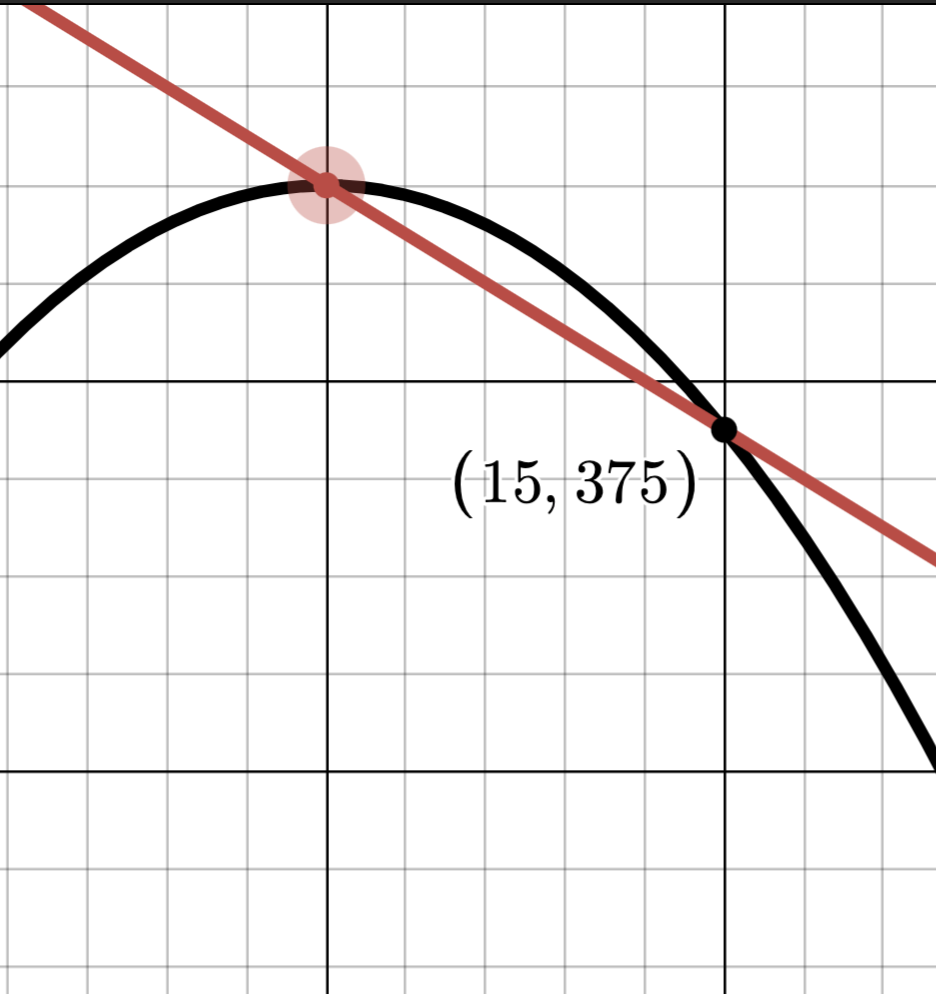
\includegraphics[width=2in]{./IntroductiontoDerivativesGraphics/sectotan01.png} &  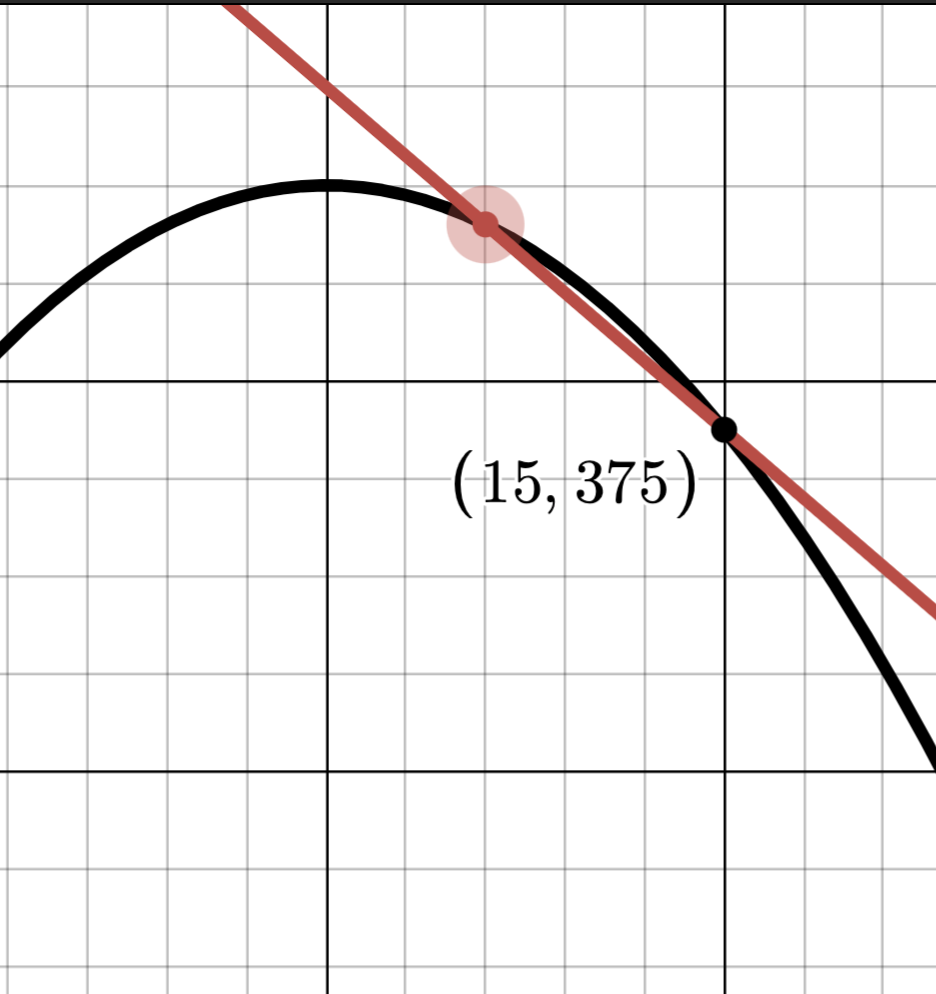
\includegraphics[width=2in]{./IntroductiontoDerivativesGraphics/sectotan03.png} &  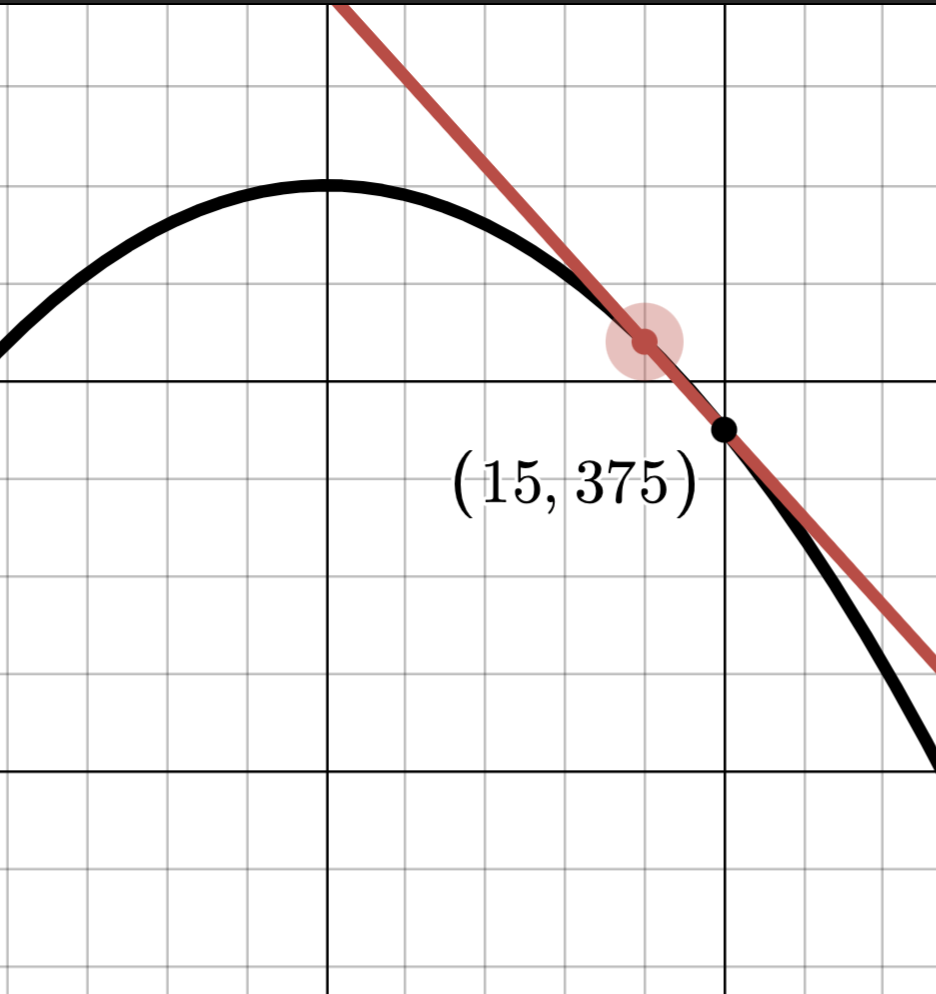
\includegraphics[width=2in]{./IntroductiontoDerivativesGraphics/sectotan05.png} \\
 
 
 \end{tabular}
 
 \end{center}
 To find the equation of the tangent line in this case, which we'll call $L(t)$,  we refer to the point-slope form of a line, Equation \ref{linearfunctionpointslope}:  \[ L(t) = s\left(t_{0} \right)+ m \left(t-t_{0} \right) = s(15) + v(15)(t-15) = 375 - 50(t-15) = -50t+1125.\]
 
The tangent line can best be thought of as `the best linear approximation' to the graph of $y = s(t)$ at $(15,375)$.  That is, if we zoom in near $(15,375)$, the graph of $y = s(t)$ and this tangent line become indistinguishable.  This geometric property of $y = s(t)$ is called \index{local linearity}\textbf{local linearity}\footnote{a.k.a. \index{differentiability}\textbf{differentiability}} and is foundational to the analysis of functions.   Below we graph $y = s(t) =  -5t^2+100t$ along with $y = L(t) = -50t + 1125$ and observe the local linearity near $(15, 375)$. 
  
  \medskip

\begin{center}

\begin{tabular}{ccc}

 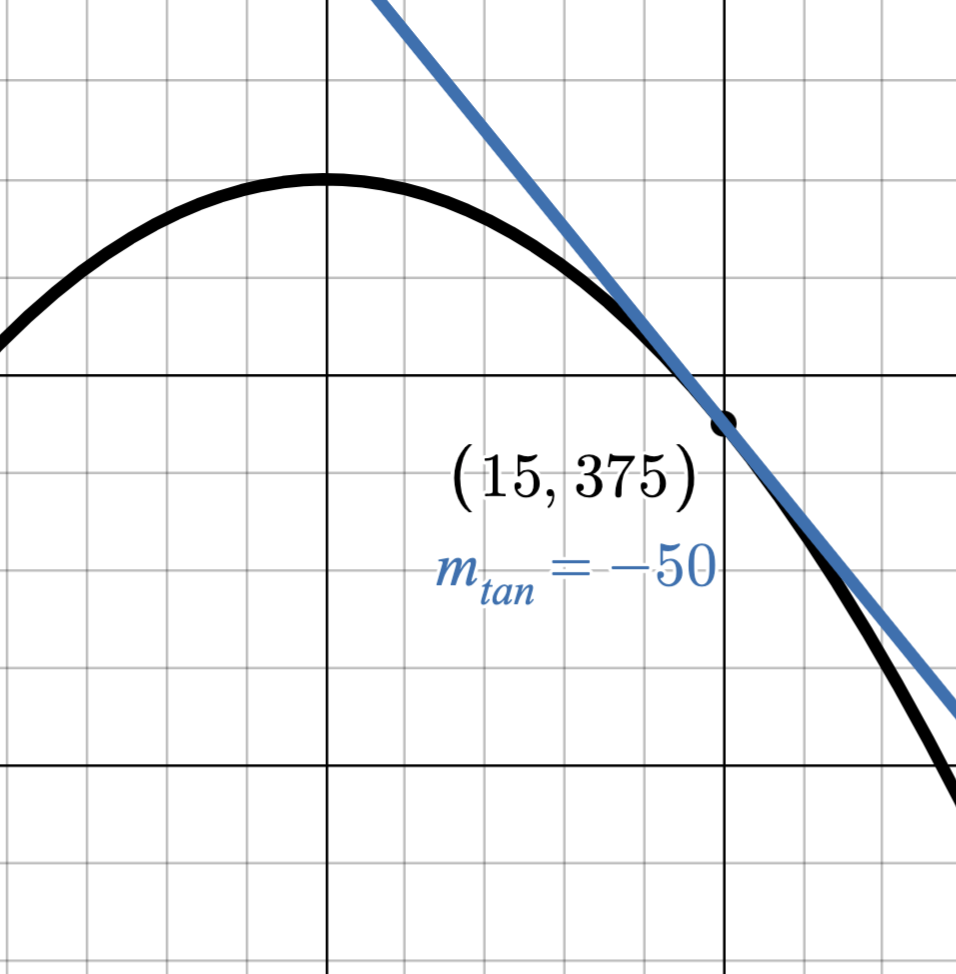
\includegraphics[width=2in]{./IntroductiontoDerivativesGraphics/tangent.png} &  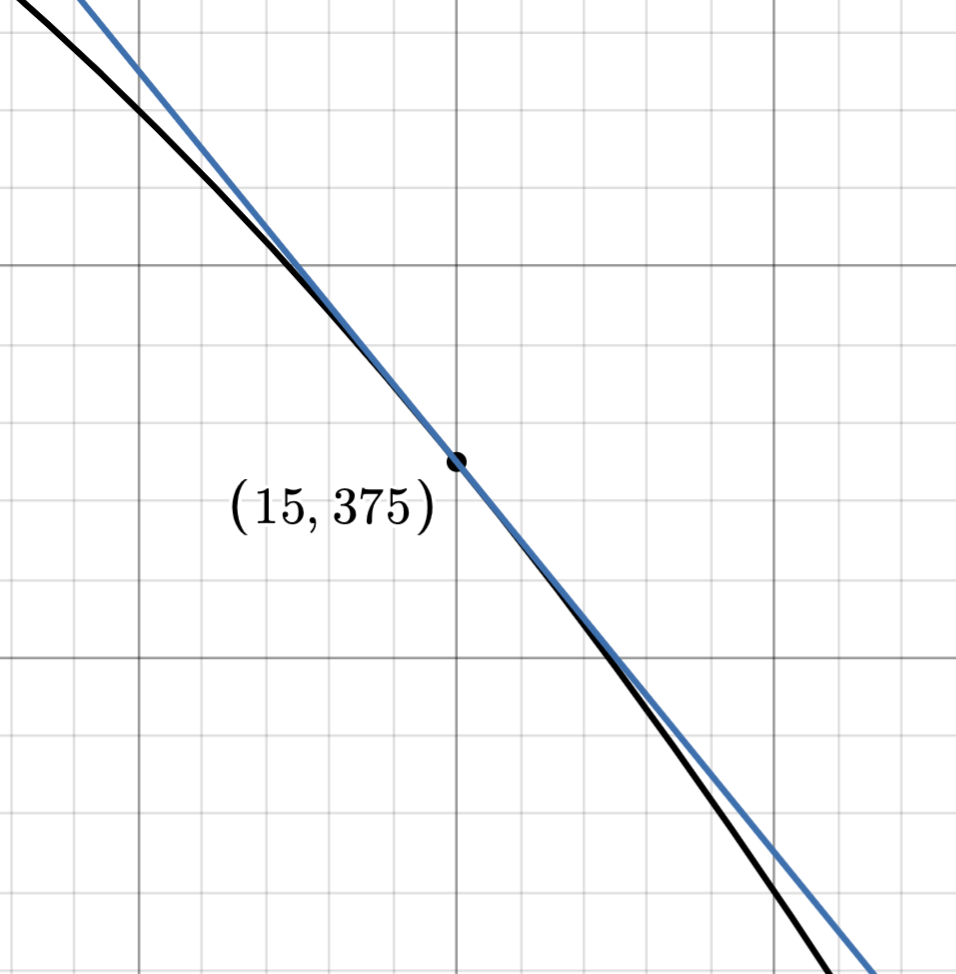
\includegraphics[width=2in]{./IntroductiontoDerivativesGraphics/tangentzoom1.png} &  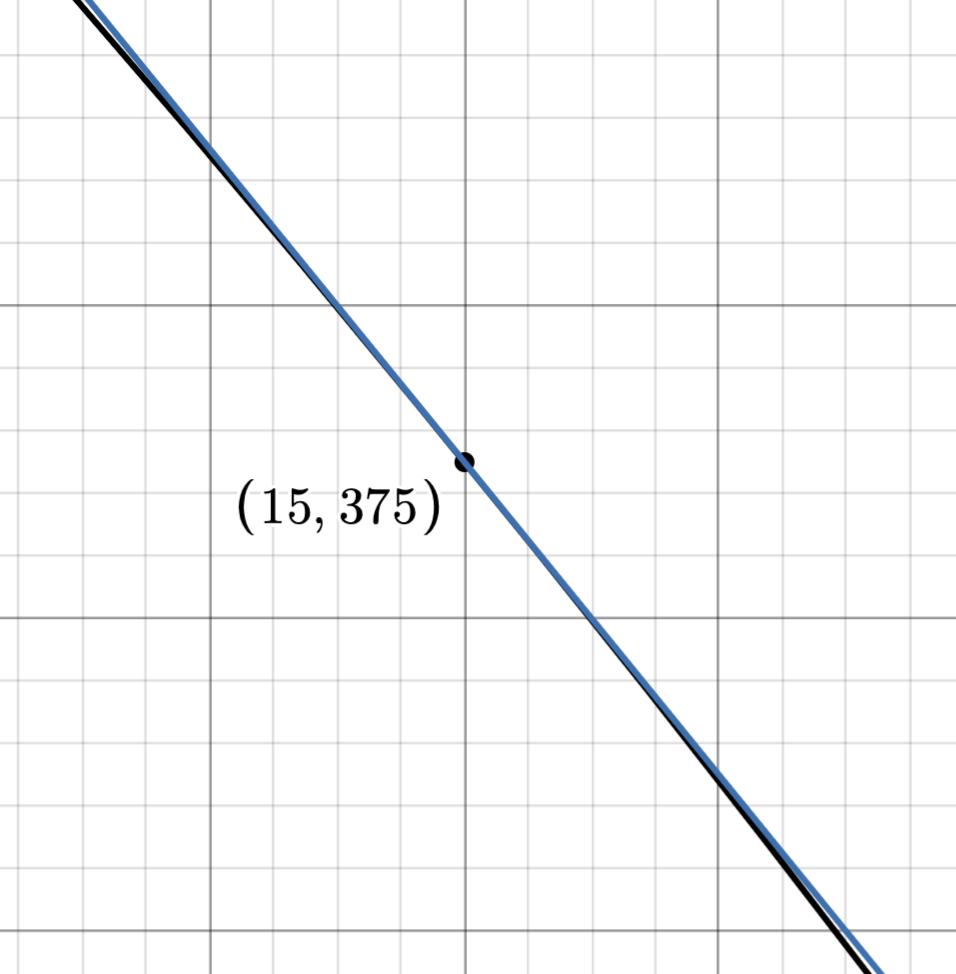
\includegraphics[width=2in]{./IntroductiontoDerivativesGraphics/tangentzoom2.png} \\
 
 The tangent line at $(15, 375)$. & Zooming in near $(15, 375)$. & Zooming in closer to $(15, 375)$. \\
 
 \end{tabular}
 
 \end{center}
 
Our next step is to generalize these notions to all functions.


\subsection{Difference Quotients and Derivatives}
\label{diffquotderiv}


Recall  in Section \ref{AverageRateofChange} the concept of the average rate of change of a function over the interval $[a,b]$  is the slope between the two points $(a, f(a))$ and $(b, f(b))$ and is given by \[ \dfrac{\Delta[f(x)]}{\Delta x} = \dfrac{f(b)-f(a)}{b-a}.\]

Geometrically, the average rate of change is the slope of the so-called \index{secant line}\textbf{secant line} which `cuts' through the graph of $y = f(x)$ at the points $(a,f(a))$ and $(b, f(b))$:

\begin{center}
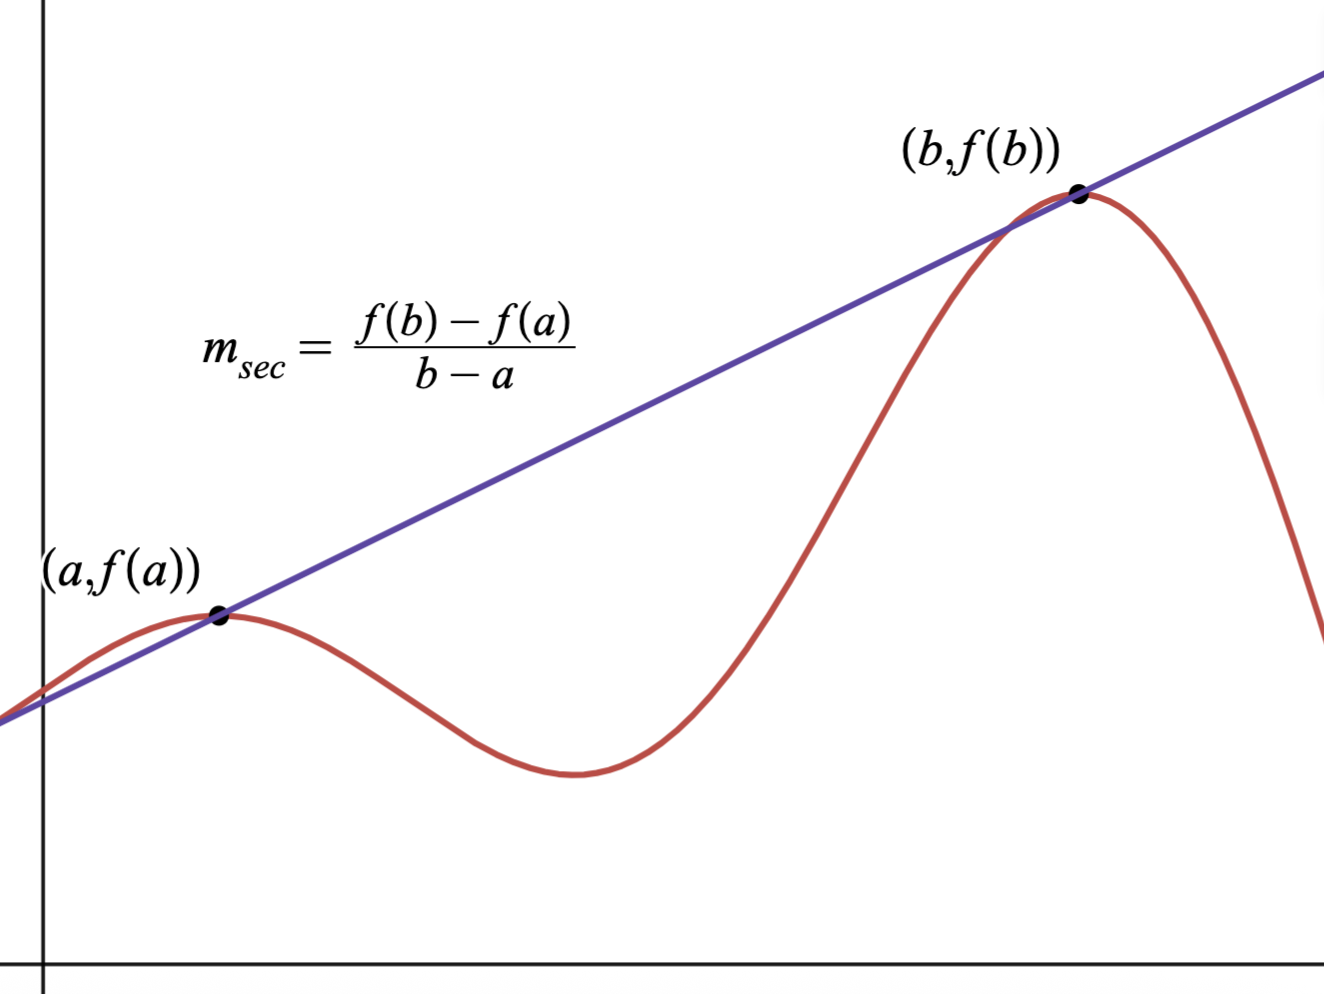
\includegraphics[width=4in]{./IntroductiontoDerivativesGraphics/SecantLine.png}
\end{center}

Consider a function $f$ defined over an interval containing $x$ and $x+h$ where $h \neq 0$. The average rate of change of $f$ over the interval $[x,x+h]$ is thus given by the formula:\footnote{assuming $h>0$;  otherwise,  the interval is $[x+h, x]$.  We get the same formula for the difference quotient either way.}

\[ \dfrac{\Delta[f(x)]}{\Delta x} = \dfrac{f(x+h)-f(x)}{h}, \quad h \neq 0.\]

The above is an example of what is traditionally called the  \index{difference quotient}\textbf{difference quotient}  or  \textbf{Newton quotient} of $f$, since it is the \textit{quotient} of two \textit{differences}, namely $\Delta[f(x)]$ and $\Delta x$. Another formula for the difference quotient (as seen in Section \ref{rocarithmetic}) keeps with the notation $\Delta x$ instead of $h$:


\[ \dfrac{\Delta[f(x)]}{\Delta x} = \dfrac{f(x+\Delta x)-f(x)}{\Delta x}, \quad \Delta x \neq 0.\]


It is important to understand that in this formulation of the difference quotient, the variables `$x$' and `$\Delta x$' are distinct - that is they do not combine as like terms. 

\medskip


Note that, regardless of which form the difference quotient takes, when $h$,  $\Delta x$, or  $\Delta t$ is $0$, the difference quotient returns the indeterminate form `$\frac{0}{0}$.' As we've seen with rational functions in Section \ref{IntroRational}, when this happens, we can use a limit to help us \textbf{determine} the \textbf{indeterminate} form.  

\medskip

In Section \ref{avginstantvelocity}, taking the limit of average velocity as $\Delta t \rightarrow 0$  produced instantaneous velocity.  More generally, taking the limit of the average rate of change  as the denominator approaches $0$ produces the \index{instantaneous rate of change}\index{rate of change ! instantaneous}\textbf{instantaneous rate of change} of the function at that point.   The instantaneous rate of change of a function, called the \index{derivative}\textbf{derivative} of the function, is defined below.

\medskip


\colorbox{ResultColor}{\bbm

\begin{defn} \label{derivativedefn} Given a function $f$ defined on an open interval containing $x=a$, the \textbf{derivative} of $f$ at $a$, denoted $f'(a)$, is defined as

\[ f'(a) = \lim_{h \rightarrow 0} \dfrac{f(a+h) - f(a)}{h}, \quad \text{provided this limit exists.} \]

 The number $f'(a)$ represents the \index{instantaneous rate of change}\index{rate of change ! instantaneous}\textbf{instantaneous rate of change} of $f$ with respect to $x$ at the input $x = a$.  If $f'(a)$ exists, we say $f$ is \index{differentiable}\textbf{differentiable} at $x = a$.

\end{defn}

\ebm}

\medskip

Using the language of derivatives, Examples \ref{averagevelocityrocketex}  and \ref{averagevelocityrocketexreprise} have us computing $v(15) = s'(15)$.   Moreover, since the derivative is a rate of change, it's important to note that the associated units of $f'(a)$ are $\frac{ \text{units of $f(x)$}}{\text{units of $x$}}$.  This tracks with the units of  $v(15) = s'(15)$ being $\frac{ \text{feet}}{\text{second}}$, a velocity.

\medskip

As in Section \ref{avginstantvelocity},  $f'(a)$ represents the slope of the tangent line at the point $(a, f(a))$.  We use this to formally define the \index{tangent line}\index{line ! tangent}\textbf{tangent line} below.

\medskip


\colorbox{ResultColor}{\bbm

\begin{defn} \label{tangentlinedefn}  If $f$ is differentiable at $x = a$, then $f'(a) =  m_{\text{tan}}$, the slope of the \index{tangent line}\index{line ! tangent}\textbf{tangent line}\textbf{tangent line} to $y = f(x)$ at $(a, f(a))$.   The equation of the tangent line is therefore:  $y = f'(a)(x-a) + f(a)$.  



\end{defn}

\ebm}

\medskip

We put these definitions to good use in the following example.

\pagebreak

\begin{ex}  \label{tangentlineex}  Let $f(x) = -x^2 + 3x-1$.  

\begin{enumerate}

\item Find the equation of the tangent line to $y = f(x)$ at $x = -2$.  Check your answer graphically.

\item  If $f$ represents the temperature (in degrees Celsius) $x$ hours after Noon on a particular day, interpret $f'(-2)$ in terms of time and temperature.

\end{enumerate}

\bigskip

{\bf Solution.}  \begin{enumerate} \item We first find $m_{\text{tan}} = f'(-2)$ using Definition \ref{derivativedefn} with $a = -2$:  $ f'(-2) = \ds{\lim_{h \rightarrow 0} \dfrac{f(-2+h) - f(-2)}{h}}$. 

First we find $f(-2+h)$ and are  careful to apply the exponent in the expression $-(-2+h)^2$:

\[ \begin{array}{rclr}  
  f(-2+h) & = & -(-2+h)^2 +3(-2+h) -1 & \\ 
  & = & - (4 - 4h+h^2) -6+3h-1 & \\
 & = & -4 + 4h-h^2-6+3h-1& \\
  & = & -h^2+7h-11& \\
 \end{array} \]

Next, we find $f(-2) = -(-2)^2 + 3(-2)-1 = -11$, so the difference quotient is:

\[ \begin{array}{rclr}

\dfrac{f(-2+h)-f(-2)}{h} & = & \dfrac{(-h^2+7h-11) -(-11)}{h} & \\[8pt]
                                & = & \dfrac{-h^2+7h}{h} & \text{simplify}\\[8pt]
                                & = &  \dfrac{h(-h+7)}{h} & \text{factor} \\[8pt]
                                & = &  \dfrac{\cancel{h}(-h+7)}{\cancel{h}} &  \text{cancel} \\[8pt]
                                & = & -h+7\\ \end{array} \]



Finally, we get $ f'(-2) = \ds{\lim_{h \rightarrow 0} \dfrac{f(-2+h) - f(-2)}{h} = \lim_{h \rightarrow 0} (-h+7) = -(0) + 7 = 7}$.

\bigskip

Hence, the slope of the tangent line is $m_{\text{tan}} = f'(-2) = 7$.  The equation of the tangent line is: 

\[ \begin{array}{rclr}  
 y & = & f'(-2)(x - (-2)) + f(-2) & \\ 
  & = & 7(x+2) - 11 & \\
 & = & 7x+14 - 11& \\
  y & = & 7x+3& \\
 \end{array} \]

Graphing $y = 7x+3$ and $y = f(x)$ near $(-2,-11)$ reveals the local linearity we would expect:

\begin{center}

\begin{tabular}{cc}

 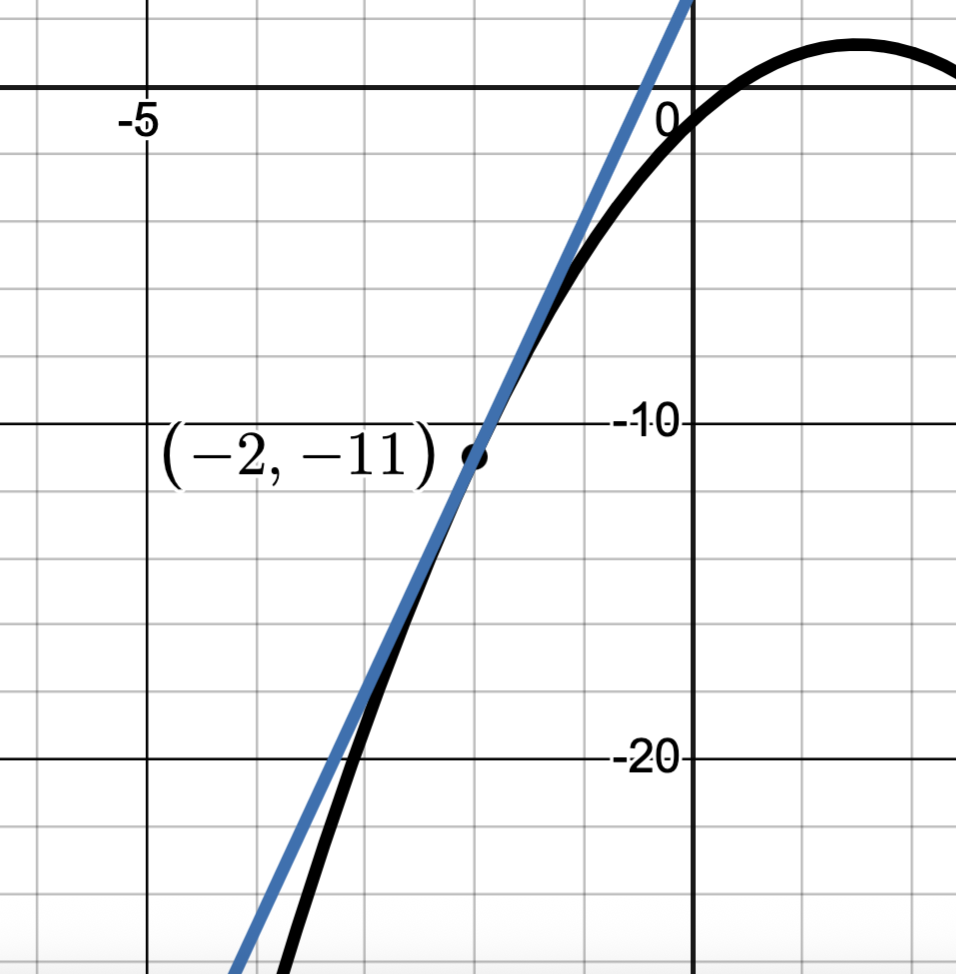
\includegraphics[width=2.5in]{./IntroductiontoDerivativesGraphics/TLEx.png} &  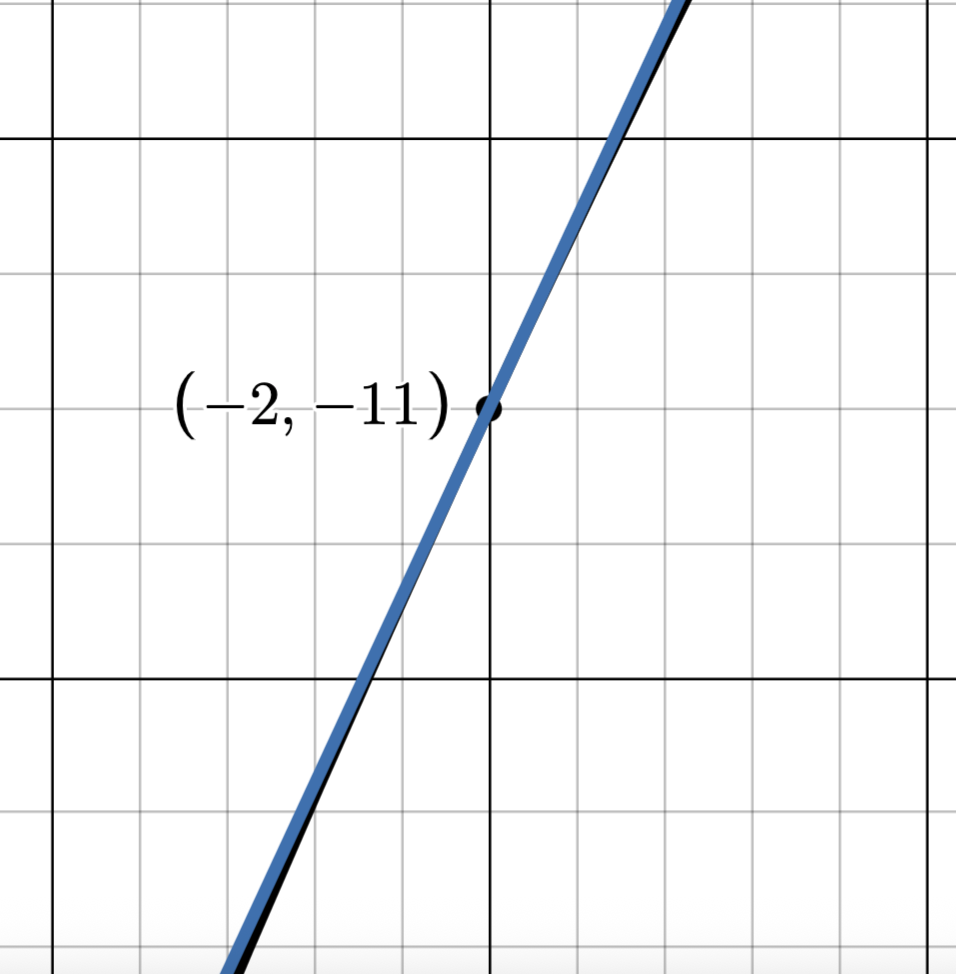
\includegraphics[width=2.5in]{./IntroductiontoDerivativesGraphics/TLExZoom.png}  \\
 
 The tangent line at $(-2,-11)$. & Zooming in near $(-2, -11)$.  \\
 
 \end{tabular}
 
 \end{center}
 
 \item Since $x$ represents the number of hours \textbf{after} Noon, $x = -2$ corresponds to $2$ hours \textbf{before} Noon, or 10 AM.  Since the units of $f(x)$ are degrees Celsius and the units of $x$ are hours, the units of $f'(-2)$ are degrees Celsius per hour.  Since $f'(-2)$ is positive, we know the slope is positive, so the temperature is increasing.  Putting all this together,   $f'(-2) = 7$ means that at 10 AM, the temperature is rising at a rate of $7$ degrees Celsius  per hour. \hfill \qed
 
 \end{enumerate}



\end{ex}

What if we wanted to find the equation of the tangent line to the graph of the function in Example \ref{tangentlineex}  at $x = 0$?  $x = 1$?  $x = 5$?  We'd ostensibly need to run through difference quotients and limit calculations for each and every input value: $x = 0$, $x = 1$, and $x = 5$.  Or we could do a single limit with a generic `$x$', simplify the difference quotient and take the limit once, and substitute in particular values of $x$:

\medskip

\colorbox{ResultColor}{\bbm

\begin{defn} \label{derivativefcndefn} Given a function $f$ defined on an open interval, the \textbf{derivative} of $f$, denoted  $f'(x)$, is the function

\[ f'(x) = \lim_{h \rightarrow 0} \dfrac{f(x+h) - f(x)}{h}, \quad \text{provided the limit exists.}\]

\end{defn}

\ebm}

\medskip

It is worth noting that if we set $h = \Delta x$, and consider the graph $y = f(x)$, we get:  \[ f'(x) = \lim_{h \rightarrow 0} \dfrac{f(x+h) - f(x)}{h} = \lim_{\Delta x \rightarrow 0} \dfrac{f(x+\Delta x) - f(x)}{\Delta x}  = \lim_{\Delta x \rightarrow 0} \dfrac{\Delta [f(x)] }{\Delta x} =  \lim_{\Delta x \rightarrow 0} \dfrac{\Delta y }{\Delta x} ,\] which is why sometimes the derivative is denoted\footnote{This is the so-called  \href{https://en.wikipedia.org/wiki/Gottfried_Wilhelm_Leibniz}{\underline{Leibniz}} notation \ldots}  $\frac{dy}{dx}$.

\pagebreak


\begin{ex}  \label{derivativeex}  Let $f(x) = -x^2 + 3x-1$.  

\begin{enumerate}

\item \label{firstpart} Find an expression for $f'(x)$.  

\item  Find $f'(-2)$ using your answer to part \ref{firstpart}   and compare that to what you obtained in Example \ref{tangentlineex}.

\item  Find the equation of the tangent line to the graph of $y = f(x)$ at $x = 0$.  Check your answer graphically.

\item  Solve $f'(x) = 0 $ and interpret your answer graphically.

\end{enumerate}

\bigskip

{\bf Solution.}

\begin{enumerate}

\item  To find  $f'(x) = \ds{ \lim_{h \rightarrow 0} \dfrac{f(x+h) - f(x)}{h}}$ we  first find $f(x+h)$:

\[ \begin{array}{rclr}  
  f(x+h) & = & -(x+h)^2 +3(x+h) -1 & \\ 
  & = & - (x^2 +2xh+h^2) +3x+3h-1 & \\
 & = & -x^2 -  2xh - h^2+3x+3h-1& \\
 \end{array} \]

The difference quotient simplifies as follows:

\[ \begin{array}{rclr}

\dfrac{f(x+h)-f(x)}{h} & = & \dfrac{( -x^2 - 2xh - h^2+3x+3h-1) -(-x^2+3x-1)}{h} & \\[8pt]
                                & = & \dfrac{-x^2 - 2xh - h^2+3x+3h-1 + x^2-3x+1}{h} & \\[8pt]
                                 & = & \dfrac{-2xh-h^2+3h}{h} & \text{simplify}\\[8pt]
                                & = &  \dfrac{h(-2x - h + 3)}{h} & \text{factor} \\[8pt]
                                & = &  \dfrac{\cancel{h}(-2x-h+3)}{\cancel{h}} &  \text{cancel} \\[8pt]
                                & = & -2x-h+3\\ \end{array} \]

Our last step is to take the limit:   $f'(x) = \ds{ \lim_{h \rightarrow 0} \dfrac{f(x+h) - f(x)}{h} = \lim_{h \rightarrow 0} (-2x-h+3)}$.  Notice here that we have two variables, $x$ and $h$, in the limit.  Of these two variables, we are taking the limit on the $h$:  $h \rightarrow 0$.  As far as $h$ is concerned, $x$ may as well be just another constant like the `$3$'.  Hence, $f'(x) = \ds{ \lim_{h \rightarrow 0} (-2x-h+3)}=  -2x - 0 + 3 = -2x+3$.

\item  Evaluating our formula for $f'(x)$ at $x = -2$ gives $f'(-2) = -2(-2) + 3 = 7$ which matches with what we obtained in Example \ref{tangentlineex}.

\item The equation of the tangent line to the graph of $y = f(x)$ at $x = 0$ is $y = f'(0) (x - 0) + f(0)$.  We have $f'(0)=2(0) + 3 = 3$ and $f(0) = -(0)^2+3(0)-1 = -1$.  We get $y = 3(x-0)+(-1)$ so $y = 3x-1$. Our graph bears this out.

\begin{center}

\begin{tabular}{cc}

 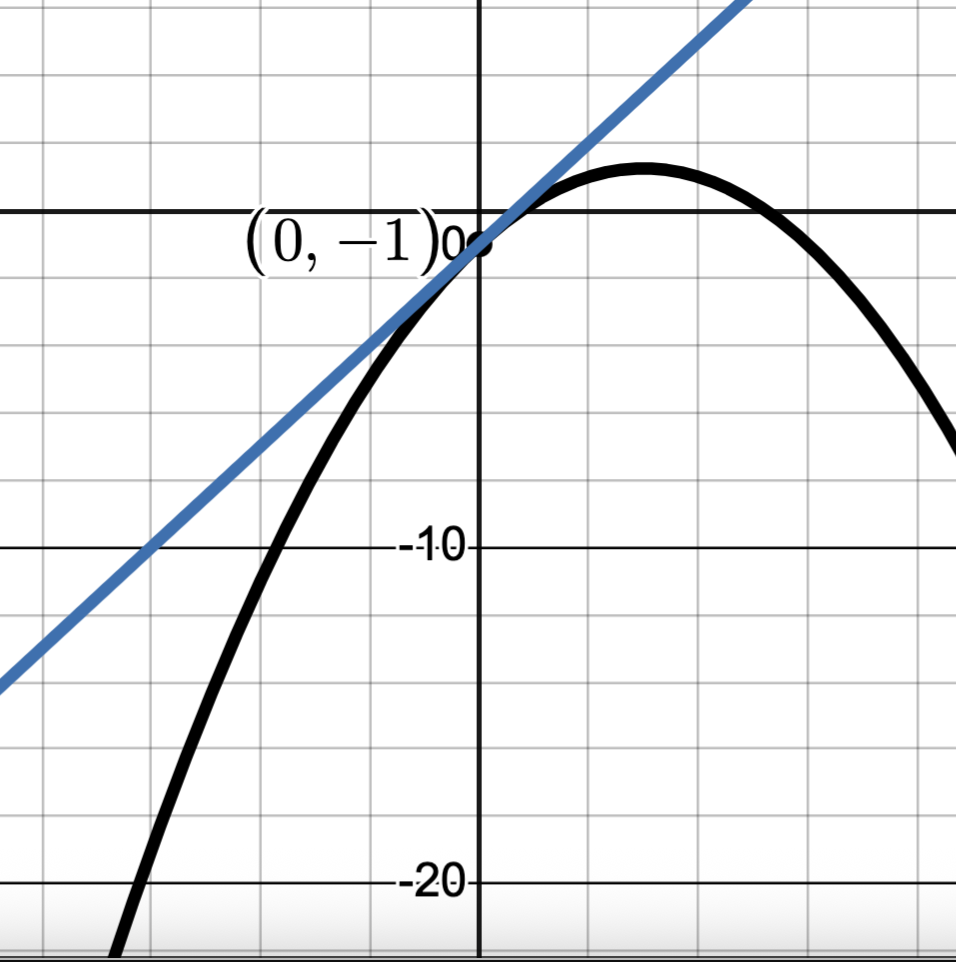
\includegraphics[width=2.5 in]{./IntroductiontoDerivativesGraphics/TL02.png} &  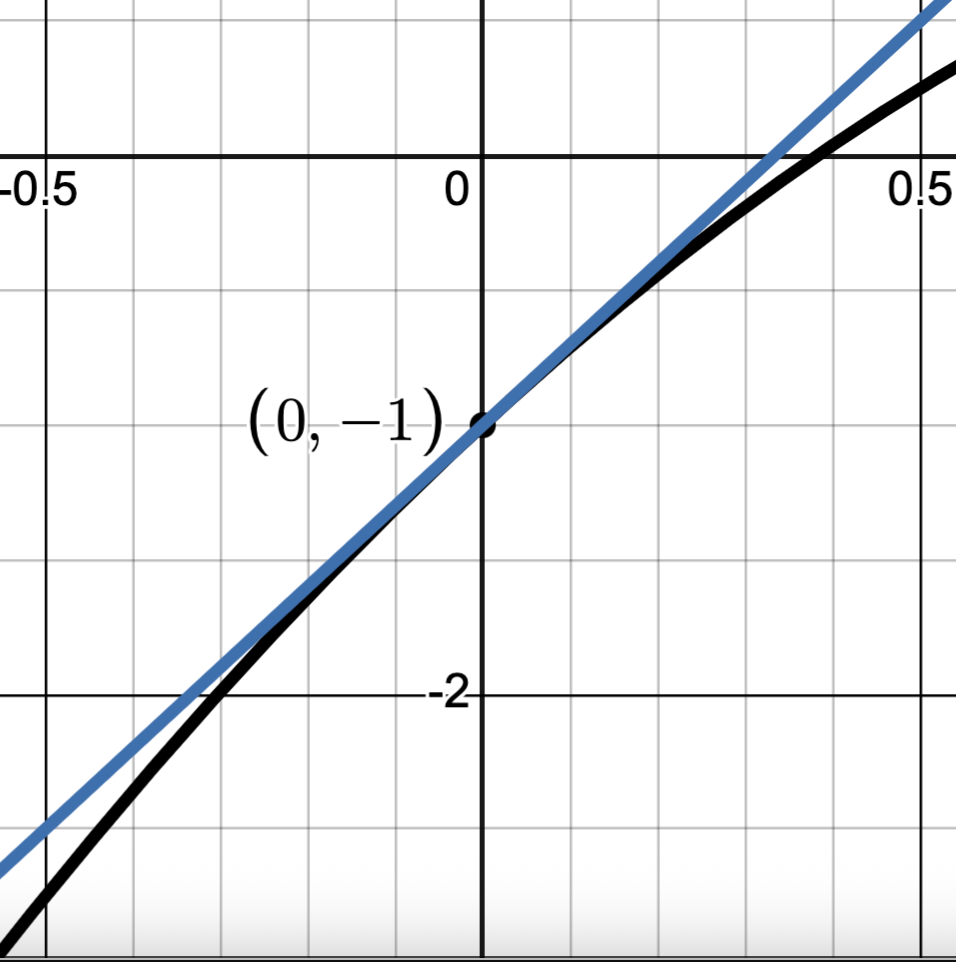
\includegraphics[width=2.5in]{./IntroductiontoDerivativesGraphics/TL02Zoom.png}  \\
 
 The tangent line at $(0,-1)$. & Zooming in near $(0, -1)$.  \\
 
 \end{tabular}
 
 \end{center}
 
 \item  Solving $f'(x) = 0$ gives $-2x+3 = 0$ so $x = \frac{3}{2}$.  This means the slope of the tangent line at the point $\left(\frac{3}{2}, f\left(\frac{3}{2}\right) \right)$ is $0$, so the tangent line there is horizontal.  We find 
 $f\left(\frac{3}{2}\right) = -\left( \frac{3}{2}\right)^2 + 3\left(\frac{3}{2}\right) - 1 = \ldots = \frac{5}{4}$.  Hence, the tangent line at  $\left(\frac{3}{2}, \frac{5}{4} \right)$ is $y = \frac{5}{4}$.  Graphically, this checks out.
 
 
 
\begin{center}

\begin{tabular}{cc}

 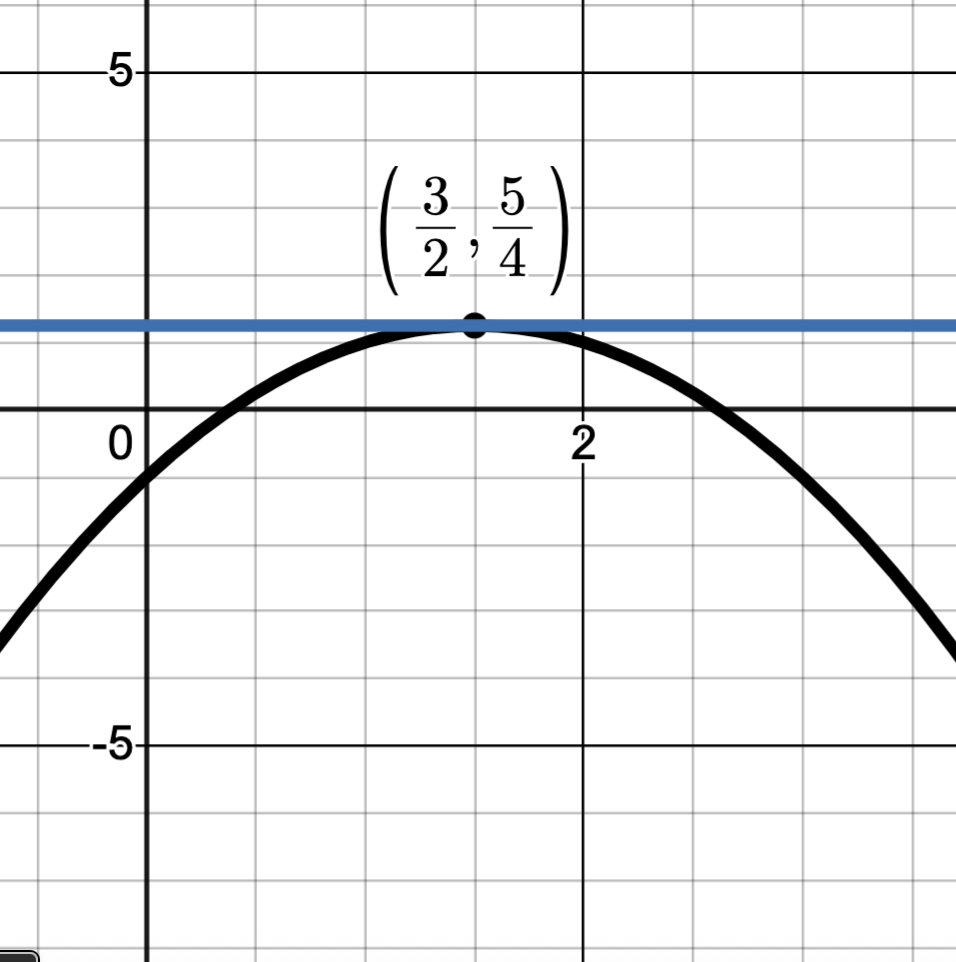
\includegraphics[width=3in]{./IntroductiontoDerivativesGraphics/HTL.png} &  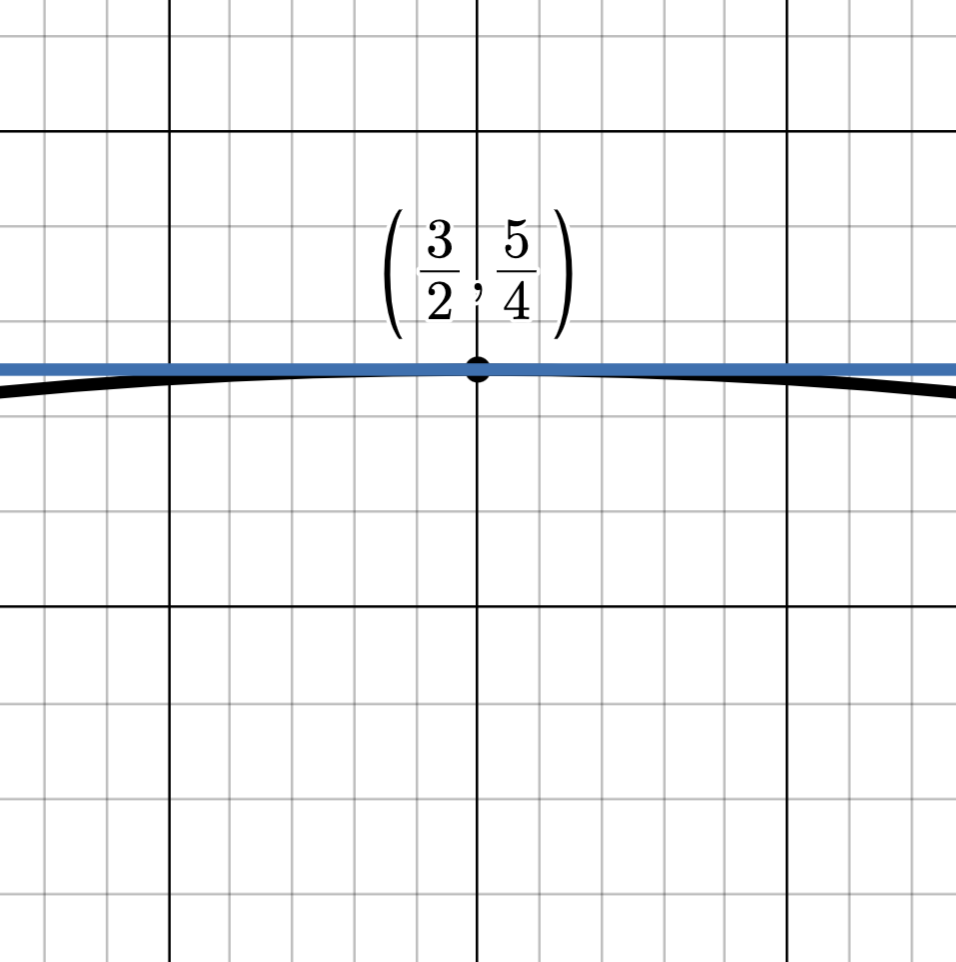
\includegraphics[width=3in]{./IntroductiontoDerivativesGraphics/HTLZoom.png}  \\
 
 The tangent line at  $\left(\frac{3}{2}, \frac{5}{4} \right)$. & Zooming in near $\left(\frac{3}{2}, \frac{5}{4} \right)$.  \\
 
 \end{tabular}
 
 \end{center}
 
 \hfill \qed


\end{enumerate}

\end{ex}

The astute reader will note that the graph of $f(x) = -x^2+3x-1$ in Example \ref{derivativeex} is a parabola and finding where $f'(x) = 0$ lead us right back to the vertex.  Using a derivative to find the vertex may seem a bit excessive given that we've algebraically derived a handy `vertex formula' in Section \ref{QuadraticFunctions}.   However, as the functions we aim to analyze become more and more sophisticated, the tools we use to analyze them must also become more sophisticated.  The derivative is one such tool that has a near universal application.\footnote{As we'll see in Section \ref{DerivativeAnalysis}.}

\medskip



\begin{ex}  \label{morederivativesex} $~$

\begin{enumerate}

\item  For $f(x) = x^2-x-2$, find and simplify:   



\begin{enumerate}

\item  $f'(3)$ %$\dfrac{f(3+h)-f(3)}{h}$ 

\item  The equation of the tangent line to the graph $y = f(x)$ at $(3, f(3))$.  

Check your answer graphically.

\item  $f'(x)$ %$\dfrac{f(x+h)-f(x)}{h}$.

\end{enumerate}



\item  For $g(x) = \dfrac{3}{2x+1}$, find and simplify:\footnote{A review of Section \ref{AppRatExpEqus} may be in order for this problem.}



\begin{enumerate}

\item  $g'(0)$ %$\dfrac{g(\Delta x)-g(0)}{\Delta x}$

\item  The equation of the tangent line to the graph $y = g(x)$ at $(0, g(0))$.  

Check your answer graphically.
 
\item  $g'(x)$ %$\dfrac{g(x+\Delta x)-g(x)}{\Delta x}$.

\end{enumerate}




\item  $r(t) = \sqrt{t}$,  find and simplify:\footnote{A review of Section \ref{rationalizingdenomandnumer} may be in order for this problem.}

\begin{enumerate}

\item $r'(9)$ %$\dfrac{r(9+\Delta t)-r(9)}{\Delta t}$ 

\item  The equation of the tangent line to the graph $y = r(t)$ at $(9, r(9))$.

 Check your answer graphically.


 \item $r'(t)$ %$\dfrac{r(t+\Delta t)- r(t)}{\Delta t}$.
 
 \end{enumerate}

\end{enumerate}



{\bf Solution.}
 
\begin{enumerate}

\item \begin{enumerate} \item To find $f'(3) = \ds{\lim_{h \rightarrow 0}}$ $\frac{f(3+h)-f(3)}{h}$ we first simplify $f(3+h)$:

\[ \begin{array}{rclr}  
  f(3+h) & = & (3+h)^2 - (3+h) -2 & \\ 
  & = & 9 + 6h+h^2 - 3 - h -2 & \\
 & = & 4 + 5h + h^2 & \\
 \end{array} \]

Since $f(3) = (3)^2-3-2 = 4$, we get for the difference quotient:

\[ \begin{array}{rclr}

\dfrac{f(3+h)-f(3)}{h} & = & \dfrac{(4 + 5h + h^2) -4}{h} & \\[8pt]
                                & = & \dfrac{5h+h^2}{h} & \\[8pt]
                                & = &  \dfrac{h(5+h)}{h} & \text{factor} \\[8pt]
                                & = &  \dfrac{\cancel{h}(5+h)}{\cancel{h}} & \text{cancel}\\[8pt]
                                & = & 5+h \\ \end{array} \]
 Hence, $f'(3) = \ds{\lim_{h \rightarrow 0} (5+h) = 5+0 = 5}$.
 
 
 \item  The equation of the tangent line at $x = 3$ is:  $y = f'(3)(x-3) + f(3) = 5(x-3) + 4$, or $y = 5x-11$. We check graphically below.
 
 \begin{center}

 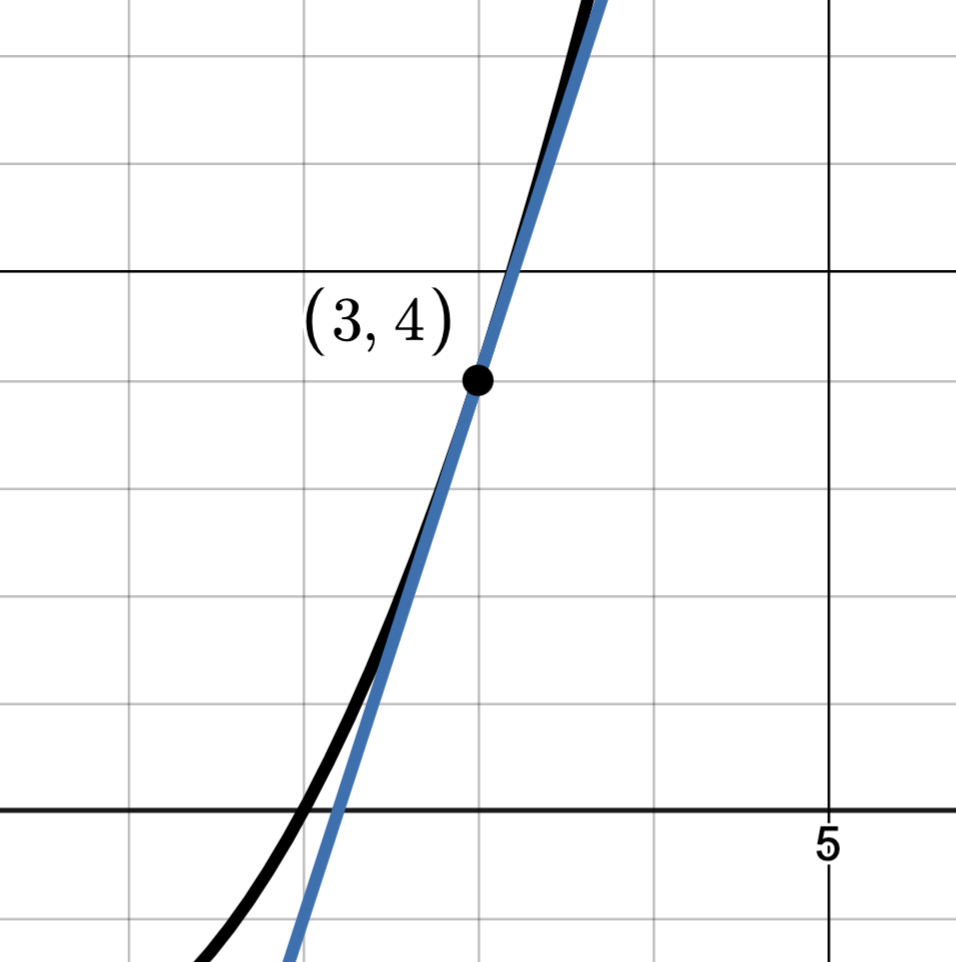
\includegraphics[width=2in]{./IntroductiontoDerivativesGraphics/TLEx201.png} 
 
 $y = f(x)$ and  $y = 5x-11$  near $(3,4)$  

 \end{center}

 \item To find $f'(x) = \ds{\lim_{h \rightarrow 0}}$ $\frac{f(x+h)-f(x)}{h}$, we first find $f(x+h)$:


\[ \begin{array}{rclr}  
 
 f(x+h) & = & (x+h)^2 - (x+h) -2 & \\ [8pt]
 & = & x^2 + 2xh + h^2 - x - h - 2.
 \end{array} \]

So the difference quotient is

\setlength{\extrarowheight}{12pt}

\begin{longtable}{rclr}  

$\dfrac{f(x+h)-f(x)}{h}$ & = & $\dfrac{\left(x^2+2xh+h^2-x-h-2 \right)-\left(x^{2}-x-2 \right)}{h}$ & \\[8pt] 
& = & $\dfrac{x^2+2xh+h^2-x-h-2-x^2+x+2}{h}$ & \\[8pt]
& = & $\dfrac{2xh+h^2-h}{h}$ & \\[8pt]
& = & $\dfrac{h \left(2x+h-1\right)}{h}$ & factor \\[8pt]
& = & $\dfrac{\cancel{h} \left(2x+h-1\right)}{\cancel{h}}$ & cancel \\[8pt]
& = & $2x+h-1$. \\

\end{longtable} 

Hence, $f'(x) = \ds{\lim_{h \rightarrow 0} (2x+h-1) = 2x + 0 - 1}$ so $f'(x) = 2x-1$. Note that using this formula, we get  $f'(3) = 2(3)-1 = 5$ which checks our answer above.


\end{enumerate}

\item  \begin{enumerate} \item Next we find  $g'(0) = \ds{\lim_{h \rightarrow 0}}$$\frac{g(0+h)-g(0)}{h}  = \frac{g(h) - g(0)}{h}$.

Since $g(h) = \frac{3}{2 h + 1}$ and $g(0) = \frac{3}{2(0)+1} = 3$, our difference quotient contains a complex fraction.  Thinking ahead, we need to (eventually) be able to cancel the factor `$h$' from the denominator $\frac{g(h) - g(0)}{h}$, so we begin by simplifying the complex fraction and see where that takes us:

\begin{longtable}{rclr}  

$\dfrac{g(0+h)-g(0)}{h}$ & = & $\dfrac{\dfrac{3}{2h+1}-3}{h}$ & \\[10pt]
& = &  $\dfrac{\dfrac{3}{2h+1}-3}{h} \cdot \dfrac{(2h+1)}{(2h+1)}$ & \\[10pt]
& = &  $\dfrac{3-3(2h+1)}{h(2h+1)}$  & \\[10pt]
& = &  $\dfrac{3 - 6 h - 3}{h(2h+1)}$  & \\[10pt]
& = &  $\dfrac{-6h}{h(2h+1)}$  & \\[10pt]
& = &  $\dfrac{-6\cancel{h}}{\cancel{h}(2h+1)}$  & \text{cancel} \\[10pt]
& = &  $\dfrac{-6}{2h+1}$.  & \\ 

\end{longtable}

We are now ready to take the limit:  \[g'(0) = \lim_{h \rightarrow 0} \frac{-6}{2h+1} = \frac{-6}{2(0)+1} = -6.\]

\item The equation of the tangent line when $x = 0$ is: $y = g'(0)(x-0) + g(0) = (-6)(x-0)+ 3$ or $y = -6x+3$, which checks graphically below.

 \begin{center}

 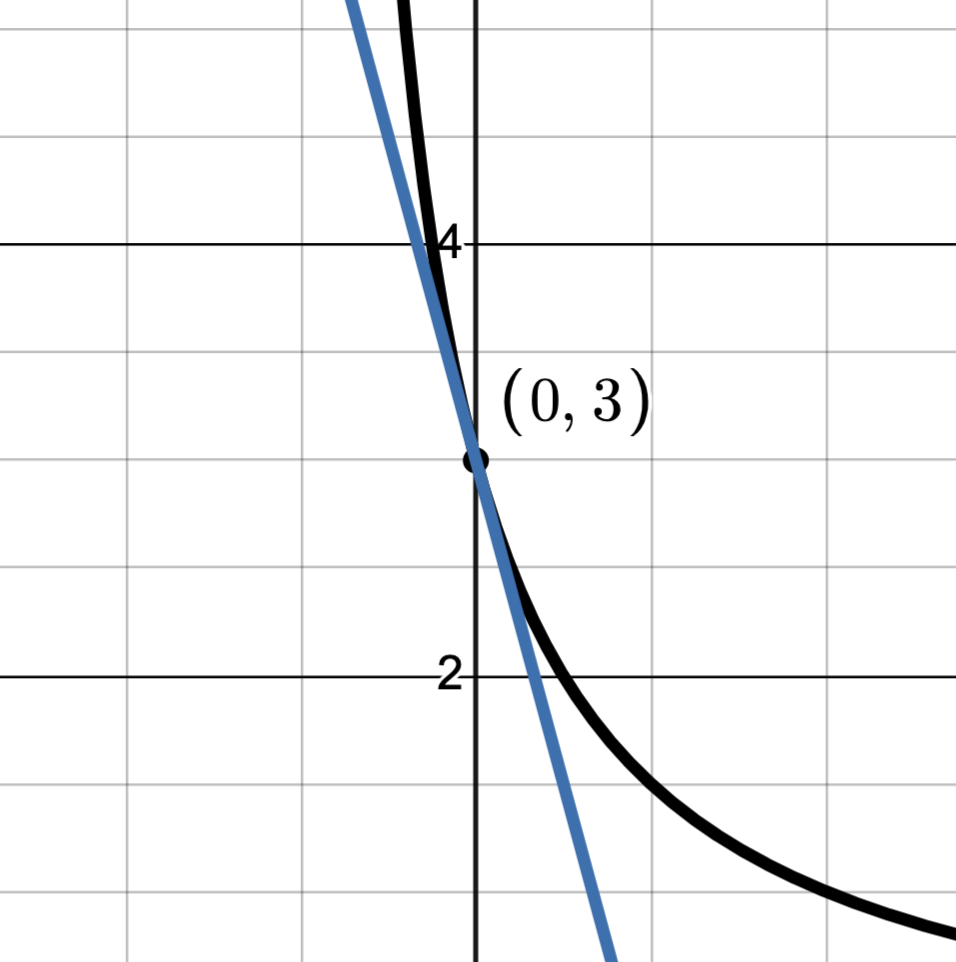
\includegraphics[width=2in]{./IntroductiontoDerivativesGraphics/TLEx202.png} 
 
 $y = g(x)$ and  $y =-6x+3$  near $(0,3)$  

 \end{center}



\item To find $g'(x)$, we first find $g(x+h)$:

 \[ \begin{array}{rclr}  
 g(x+h) & = & \dfrac{3}{2(x+h)+1} & \\[10pt]
 & = & \dfrac{3}{2x+2h+1} \\
 \end{array} \]

Simplifying the difference quotient involves simplifying the resulting complex fraction, as above, keeping an eye out for an opportunity to cancel the factor `$h$' from the denominator:

\begin{longtable}{rclr}  

$\dfrac{g(x+h)-g(x)}{h}$ & = & $\dfrac{\dfrac{3}{2x+2h+1}-\dfrac{3}{2x+1}}{h}$ & \\[10pt]
& = &  $\dfrac{\dfrac{3}{2x+2h+1}-\dfrac{3}{2x+1}}{h} \cdot \dfrac{(2x+2h+1)(2x+1)}{(2x+2h+1)(2x+1)}$ & \\[10pt]
& = &  $\dfrac{3(2x+1)-3(2x+2h+1)}{h(2x+2h+1)(2x+1)}$  & \\[10pt]
& = &  $\dfrac{6x+3-6x-6h-3}{h(2x+2h+1)(2x+1)}$  & \\[10pt]
& = &  $\dfrac{-6h}{h(2x+2h+1)(2x+1)}$  & \\[10pt]
& = &  $\dfrac{-6\cancel{h}}{\cancel{h}(2x+2h+1)(2x+1)}$  & \text{cancel} \\[10pt]
& = &  $\dfrac{-6}{(2x+2h+1)(2x+1)}$.  & \\ 

\end{longtable}

Hence, \[g'(x) = \lim_{h \rightarrow 0} \frac{-6}{(2x+2h+1)(2x+1)} = \frac{-6}{(2x + 2(0) +1)(2x+1)} = - \frac{6}{(2x+1)^2}. \]   We check $g'(0) = -\frac{6}{(2(0)+1)^2} = \ldots = -6$, as required.

\end{enumerate}



\item \begin{enumerate} \item To find $r'(9) = \ds{\lim_{h \rightarrow 0}}$$\frac{r(9+h) - r(9)}{h}$, we start with $r(9+h) = \sqrt{9+h}$ and $r(9) = \sqrt{9} = 3$. Hence  our difference quotient is:

\[ \dfrac{r(9+h)-r(9)}{h} = \dfrac{\sqrt{9+h} - 3}{h}.\]


In order for us to determine the limit as $h \rightarrow 0$, we need to somehow cancel the factor of $h$ from the  \textbf{denominator}.  To do so,  we set about \textbf{rationalizing the numerator} by multiplying both numerator and denominator by the conjugate\footnote{Again, see Section  \ref{rationalizingdenomandnumer} for a review of these sorts of machinations.}of the numerator, $\sqrt{9+h} - 3$:


\[ \begin{array}{rcll}  

\dfrac{r(9+h) - r(9)}{h} & = & \dfrac{\sqrt{9+h} - 3}{h} & \\[15pt]
												
												 & = & \dfrac{\left(\sqrt{9+h} - 3 \right)}{h} \cdot \dfrac{\left(\sqrt{9+h} + 3\right)}{\left(\sqrt{9+h} + 3\right)} & \text{Multiply by the conjugate.} \\[15pt]
										
												 & = &  \dfrac{\left(\sqrt{9+h}\right)^2 -(3)^2}{h\left(\sqrt{9+h} + 3\right)} & \text{Difference of Squares.}\\[15pt]
												
												& = &  \dfrac{(9+h) - 9}{h\left(\sqrt{9+h} + 3\right)} & \\[15pt]
												
												 & = &  \dfrac{h}{h\left(\sqrt{9+h} + 3\right)} & \\[15pt]
												 
												 & = &  \dfrac{\cancelto{1}{h}}{\cancel{h}\left(\sqrt{9+h} + 3\right)} & \text{cancel} \\[15pt]
										
										
												 & = &  \dfrac{1}{\sqrt{9+h} +3} & \\ 
												\end{array}\]	


Hence, \[ r'(9) = \lim_{h \rightarrow 0} \frac{1}{\sqrt{9+h} +3} = \frac{1}{\sqrt{9+0} +3} = \frac{1}{6}.\]

\item  The equation of the tangent line to $y = r(t)$ at $(9,3)$ is therefore:  $y = r'(9)(t-9) + r(9) = \frac{1}{6} (t-9) + 3$ or $y = \frac{1}{6} \, t + \frac{3}{2}$. The graph below confirms this.

 \begin{center}

 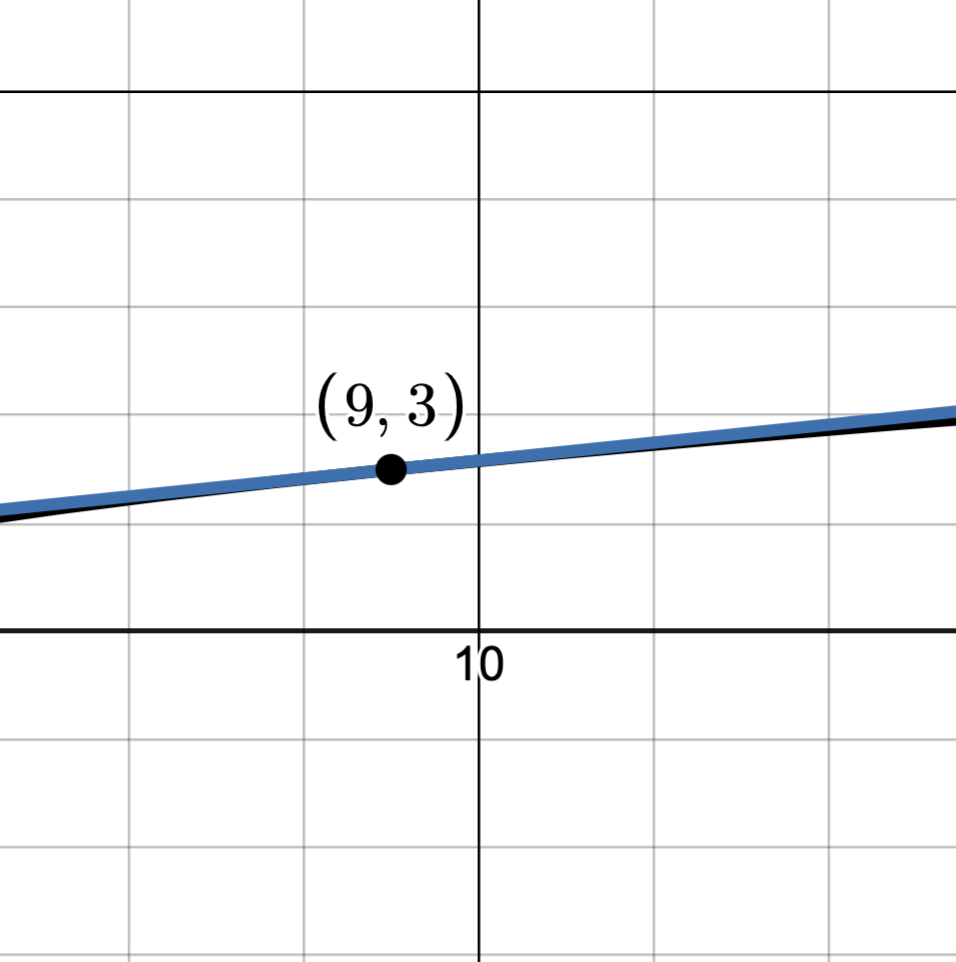
\includegraphics[width=2in]{./IntroductiontoDerivativesGraphics/TLEx203.png} 
 
 $y =r(t)$ and   $y = \frac{1}{6} \, t + \frac{3}{2}$  near $(9,3)$  

 \end{center}

\item As one might expect, we use this same strategy of rationalizing the numerator to simplify the difference quotient to find $r'(t)$:

\[ \begin{array}{rcll}  

\dfrac{r(t+h) - r(t)}{h} & = & \dfrac{\sqrt{t+h} - \sqrt{t}}{h} & \\ [15pt]
												
												 & = & \dfrac{\left(\sqrt{t+h} - \sqrt{t}\right)}{h} \cdot \dfrac{\left(\sqrt{t+h} + \sqrt{t}\right)}{\left(\sqrt{t+h} + \sqrt{t}\right)} & \text{Multiply by the conjugate.} \\ [15pt]
										
												 & = &  \dfrac{\left(\sqrt{t+h}\right)^2 - \left(\sqrt{t}\right)^2}{h\left(\sqrt{t+h} + \sqrt{t}\right)} & \text{Difference of Squares.}\\ [15pt]
												
												& = &  \dfrac{(t+h) - t}{h\left(\sqrt{t+h} + \sqrt{t}\right)} & \\ [15pt]
												
												 & = &  \dfrac{h}{h\left(\sqrt{t+h} + \sqrt{t}\right)} & \\ [15pt]
												 
												 												 & = &  \dfrac{\cancelto{1}{h}}{\cancel{h}\left(\sqrt{t+h} + \sqrt{t}\right)} & \\ [15pt]
										
										
												 & = &  \dfrac{1}{\sqrt{t+h} + \sqrt{t}} & \\ 
												\end{array}\]	


We get \[r'(t) =  \lim_{h \rightarrow 0} \frac{1}{\sqrt{t+h} + \sqrt{t}} = \frac{1}{\sqrt{t+0} + \sqrt{t}}  = \frac{1}{2 \sqrt{t}}.\]   We check $r'(9) = \frac{1}{2\sqrt{9}} = \frac{1}{2(3)} = \frac{1}{6}$ as above.  \hfill \qed

\end{enumerate}

\end{enumerate}

\end{ex}




\newpage


\subsection{Exercises}

%% SKIPPED %% \label{ExercisesforAppDerivatives}
In Exercises \ref{diffquotexerfirsta} - \ref{diffquotexerlasta}, find the limit of the following difference quotients.

\begin{multicols}{2}

\begin{itemize}

\item  $\ds{\lim_{h \rightarrow 0} \dfrac{f(2+h) - f(2)}{h}}$

\item  $\ds{\lim_{h \rightarrow 0} \dfrac{f(x+h) - f(x)}{h}}$

\end{itemize}

\end{multicols}


\begin{multicols}{2}

\begin{enumerate}


\item $f(x) = 2x - 5$ \label{diffquotexerfirsta}
\item $f(x) = -3x + 5$

\setcounter{HW}{\value{enumi}}
\end{enumerate}
\end{multicols}

\begin{multicols}{2}
\begin{enumerate}
\setcounter{enumi}{\value{HW}}

\item $f(x) = 6$
\item $f(x) = 3x^2 - x$

\setcounter{HW}{\value{enumi}}
\end{enumerate}
\end{multicols}

\begin{multicols}{2}
\begin{enumerate}
\setcounter{enumi}{\value{HW}}

\item $f(x) = -x^2 + 2x - 1$
\item\label{diffquotexerlasta}  $f(x) = 4x^2$ 

\setcounter{HW}{\value{enumi}}
\end{enumerate}
\end{multicols}


In Exercises \ref{tangentlinepolyfirst} - \ref{tangentlinepolylast}, find:


\begin{itemize}

\item  $f'(2)  = \ds{\lim_{h \rightarrow 0} \dfrac{f(2+h) - f(2)}{h}}$

\item  The equation of the tangent line at $(2, f(2))$.  Check your answer graphically.

\item  $f'(x) = \ds{\lim_{h \rightarrow 0} \dfrac{f(x+h) - f(x)}{h}}$

\item  The equation of the tangent line at $(0,f(0))$.  Check your answer graphically.
 
\end{itemize}



\begin{multicols}{2}
\begin{enumerate}
\setcounter{enumi}{\value{HW}}

\item\label{tangentlinepolyfirst}  $f(x) = x-x^2$ 
\item\label{tangentlinepolylast} $f(x) = x^{3} + 1$

\setcounter{HW}{\value{enumi}}
\end{enumerate}
\end{multicols}




\begin{enumerate}
\setcounter{enumi}{\value{HW}}

\item  Find $f'(x) = \ds{\lim_{h \rightarrow 0} \dfrac{f(x+h) - f(x)}{h}}$  for $f(x) = mx + b\;$ where $m \neq 0$

\item\label{quadraticderivativeformulaexercise} \begin{enumerate}  \item Find $f'(x) = \ds{\lim_{h \rightarrow 0} \dfrac{f(x+h) - f(x)}{h}}$   for  $f(x) = ax^{2} + bx + c\;$ where $a \neq 0$.

\item  Solve $f'(x) = 0$ for $x$.  Does this look familiar?  Explain.

\end{enumerate}

\setcounter{HW}{\value{enumi}}
\end{enumerate}





In Exercises \ref{diffquotexerfirstb} - \ref{diffquotexerlastb}, find the limit of the following difference quotients:

\begin{multicols}{2}

\begin{itemize}

\item  $\ds{\lim_{\Delta x \rightarrow 0} \dfrac{f(-1+\Delta x) - f(-1)}{\Delta x}}$

\item  $\ds{\lim_{\Delta x \rightarrow 0} \dfrac{f(x+\Delta x) - f(x)}{\Delta x}}$

\end{itemize}

\end{multicols}

\begin{multicols}{2}
\begin{enumerate}
\setcounter{enumi}{\value{HW}}

\item $f(x) = \dfrac{2}{x}$  \label{diffquotexerfirstb}
\item $f(x) = \dfrac{3}{1-x}$

\setcounter{HW}{\value{enumi}}
\end{enumerate}
\end{multicols}

\begin{multicols}{2}
\begin{enumerate}
\setcounter{enumi}{\value{HW}}

\item  $f(x) = \dfrac{1}{x^2}$
\item\label{diffquotexerlastb}  $f(x) = \dfrac{2}{x+5}$

\setcounter{HW}{\value{enumi}}
\end{enumerate}
\end{multicols}

In Exercises \ref{rationaltangentfirst} - \ref{rationaltangentlast}, find the limit of the following:



\begin{itemize}

\item  $f'(-1) = \ds{\lim_{\Delta x \rightarrow 0} \dfrac{f(-1+\Delta x) - f(-1)}{\Delta x}}$

\item The equation of the tangent line at $(-1, f(-1))$.

\item  $f'(x) = \ds{\lim_{\Delta x \rightarrow 0} \dfrac{f(x+\Delta x) - f(x)}{\Delta x}}$

\item  The equation of the tangent line at $(0,f(0))$.

\end{itemize}

\begin{multicols}{2}
\begin{enumerate}

\setcounter{enumi}{\value{HW}}

\item\label{rationaltangentfirst} $f(x) = \dfrac{1}{4x-3}$ 
\item $f(x) = \dfrac{3x}{x+2}$ 

\setcounter{HW}{\value{enumi}}
\end{enumerate}
\end{multicols}

\begin{multicols}{2}
\begin{enumerate}
\setcounter{enumi}{\value{HW}}

\item $f(x) = \dfrac{x}{x - 9}$
\item\label{rationaltangentlast} $f(x) = \dfrac{x^2}{2x+1}$ 

\setcounter{HW}{\value{enumi}}
\end{enumerate}
\end{multicols}

In Exercises \ref{diffquotexerfirstc} - \ref{diffquotexerlastc},  find the limit of the following difference quotients:

\begin{multicols}{2}

\begin{itemize}

\item  $\ds{\lim_{\Delta t \rightarrow 0} \dfrac{g(\Delta t) - g(0)}{\Delta t}}$

\item  $\ds{\lim_{\Delta t \rightarrow 0} \dfrac{g(t+\Delta t) - g(t)}{\Delta t}}$

\end{itemize}

\end{multicols}


\begin{multicols}{2}
\begin{enumerate}
\setcounter{enumi}{\value{HW}}

\item  $g(t) = \sqrt{9-t}$  \label{diffquotexerfirstc}
\item  $g(t) = \sqrt{2t+1}$   \label{diffquotexerlastc}


\setcounter{HW}{\value{enumi}}
\end{enumerate}
\end{multicols}

In Exercises \ref{tangentrootfirst} - \ref{tangentrootlast},  find the following:



\begin{itemize}

\item  $g'(0) = \ds{\lim_{\Delta t \rightarrow 0} \dfrac{g(\Delta t) - g(0)}{\Delta t}}$

\item  The equation of the tangent line at $(0, g(0))$.

\item  $g'(t) =  \ds{\lim_{\Delta t \rightarrow 0} \dfrac{g(t+\Delta t) - g(t)}{\Delta t}}$

\item  The equation of the tangent line at $(1, g(1))$.

\end{itemize}




\begin{multicols}{2}
\begin{enumerate}
\setcounter{enumi}{\value{HW}}

\item\label{tangentrootfirst}  $g(t) = \sqrt{-4t+5}$
\item  \label{tangentrootlast} $g(t) = \sqrt{4-t}$


\setcounter{HW}{\value{enumi}}
\end{enumerate}
\end{multicols}



\begin{enumerate}
\setcounter{enumi}{\value{HW}}

\item  For  $g(t) = t \sqrt{t}$:

\begin{enumerate}

\item  Explain why $g'(0) = \ds{\lim_{\Delta t \rightarrow 0} \dfrac{g(\Delta t) - g(0)}{\Delta t}}$ does not exist.

\item Find the \index{derivative from the right}\index{derivative ! from the right} derivative \textbf{from the right} at $t=0$:  $g_{+}'(0) = \ds{\lim_{\Delta t \rightarrow 0^{+}} \dfrac{g(\Delta t) - g(0)}{\Delta t}}$

\item  Find $y = g_{+}'(0) (x-0) + g(0)$ and interpret.

\item Find  $g'(t) =  \ds{\lim_{\Delta t \rightarrow 0} \dfrac{g(t+\Delta t) - g(t)}{\Delta t}}$.  Assume $t>0$.

\end{enumerate}


\item  \begin{enumerate} \item Find  $g'(t) =  \ds{\lim_{\Delta t \rightarrow 0} \dfrac{g(t+\Delta t) - g(t)}{\Delta t}}$ for  $g(t) = \sqrt{at+b}$, $a \neq 0$. 

\smallskip

\item What restrictions do you place on $t$ so your formula is valid?

\end{enumerate}


\setcounter{HW}{\value{enumi}}
\end{enumerate}


\begin{enumerate}
\setcounter{enumi}{\value{HW}}

\item Let  $f(x) =|x|$.  

\begin{enumerate}

\item  Explain why $f$ is continuous at $x = 0$.

\item\label{cornerex} Show $f'(0)$ does not exist by showing $\ds{\lim_{h \rightarrow 0^{-}} \dfrac{f(h) - f(0)}{h} =-1}$ but  $\ds{\lim_{h \rightarrow 0^{+}} \dfrac{f(h) - f(0)}{h} = 1}$.  

\smallskip
        
\item  Graph $y = f(x)$ near $(0,0)$.  Interpret your answer to number \ref{cornerex} graphically.

\smallskip

\item  Find and simplify  $f'(x) =  \ds{\lim_{h \rightarrow 0} \dfrac{|x+h| - |x|}{h}}$ assuming $x \neq 0$.

\smallskip

\textbf{HINT:}  Consider the two cases $x > 0$ and $x < 0$ \ldots
        
\smallskip

\end{enumerate}


\item Let  $g(t) = \sqrt[3]{t}$.  

\begin{enumerate}

\item Explain why $g$ is continuous at $t = 0$.

\item\label{verticaltangentex} Show $g'(0)$ does not exist by showing $\ds{\lim_{\Delta t \rightarrow 0} \dfrac{g(\Delta t) - g(0)}{\Delta t} = \infty}$.  

\smallskip
        
\item  Graph $y = g(t)$ near $(0,0)$.  Interpret your answer to number \ref{verticaltangentex} graphically.

\smallskip

\item  Find and simplify  $g'(t) =  \ds{\lim_{\Delta t \rightarrow 0} \dfrac{g(t+\Delta t) - g(t)}{\Delta t}}$ assuming $t \neq 0$.

\smallskip

\textbf{HINT:}  $(a-b)\left(a^2+ab+b^2\right) = a^3 - b^3$ 
        
\smallskip

\end{enumerate}

\item Let  $h(x) = x^{\frac{2}{3}}$.  

\begin{enumerate}

\item Explain why $h$ is continuous at $x = 0$.

\item\label{cuspex} Show $h'(0)$ does not exist by showing $\ds{\lim_{\Delta x \rightarrow 0^{-}} \dfrac{h(\Delta x) - h(0)}{\Delta x} = -\infty}$ and $\ds{\lim_{\Delta x \rightarrow 0^{+}} \dfrac{h(\Delta x) - h(0)}{\Delta x} = \infty}$

\smallskip
        
\item  Graph $y = h(x)$ near $(0,0)$.  Interpret your answer to number \ref{cuspex} graphically.

\smallskip

\item  Find and simplify  $h'(x) =  \ds{\lim_{\Delta x \rightarrow 0} \dfrac{h(x+\Delta x) - h(x)}{\Delta x}}$ assuming $x \neq 0$.

\smallskip

\textbf{HINT:}  $(a-b)\left(a^2+ab+b^2\right) = a^3 - b^3$ and $a^2 - b^2 = (a+b)(a-b)$.
        
\smallskip

\end{enumerate}

\item  Recall from Exercise \ref{JasonHammerExercise1} in Section \ref{QuadraticFunctions} that Carl's friend Jason participates in the Highland Games. In one event, the hammer throw, the height $h(t)$ in feet of the hammer above the ground $t$ seconds after Jason lets it go is modeled by the function $h(t) = -16t^2 +  22.08t + 6$. 

\begin{enumerate}

\item  Find and simplify a formula for the velocity of the hammer, $v(t) = h'(t) = \ds{\lim_{\Delta t \rightarrow 0} \dfrac{h(t + \Delta t) - h(t)}{\Delta t}}$.

\item  Find and interpret $v(0)$.

\item  Solve $v(t) = 0$ and interpret.

\item  Find the velocity of the hammer when it hits the ground, rounded to three decimal places.

\end{enumerate}

\item  In Exercise \ref{fueleconomyexercise}  in Section \ref{QuadraticFunctions}, the average fuel economy $F(t)$ in miles per gallon (mpg) for passenger cars in the US $t$ years after 1980 is modeled by  $F(t) = -0.0076t^2+0.45t + 16$, $0 \leq t \leq 28$. 

\begin{enumerate}

\item  Find and simplify a formula for  $F'(t) = \ds{\lim_{h \rightarrow 0} \dfrac{F(t + h) - F(t)}{h}}$.

\item\label{fueleconomytrendexercise}  Find and interpret $F'(0)$, $F'(5)$ and $F'(10)$.

\item  Interpret the trend you observe in your answers to part \ref{fueleconomytrendexercise}.

\end{enumerate}

\item\label{MarginalCostDerivativeExercise} Let us return to Example \ref{marginalsetupex} where  $C(x) = .03x^{3} - 4.5x^{2} + 225x + 250$ denotes the cost, in dollars,  of producing $x$ PortaBoy game systems.

\begin{enumerate}

\item  Find and interpret $C'(75) = \ds{\lim_{h \rightarrow 0} \dfrac{C(75+h) - C(75)}{h}}$.

\item  Recall in Exercise \ref{AverageCostMarginalCostExercise} in Section \ref{FunctionArithmetic}, we found the marginal cost, $MC(75) = 58.53$,   which means it will cost an additional $\$ 58.53$ to produce the $76$th item.  Compare $C'(75)$ and $MC(75)$. 

\end{enumerate}

\setcounter{HW}{\value{enumi}}
\end{enumerate}

\newpage


In Exercises \ref{MatchFcnDerivative1first} - \ref{MatchFcnDerivative1last}, match the graph of the function with a plausible graph of its derivative.

\begin{center}

\begin{multicols}{2}

\begin{enumerate}
\setcounter{enumi}{\value{HW}}

\item \label{MatchFcnDerivative1first}$y = f(x)$:

\setcounter{HW}{\value{enumi}}
\end{enumerate}

Graph A:

\end{multicols}


\begin{multicols}{2}

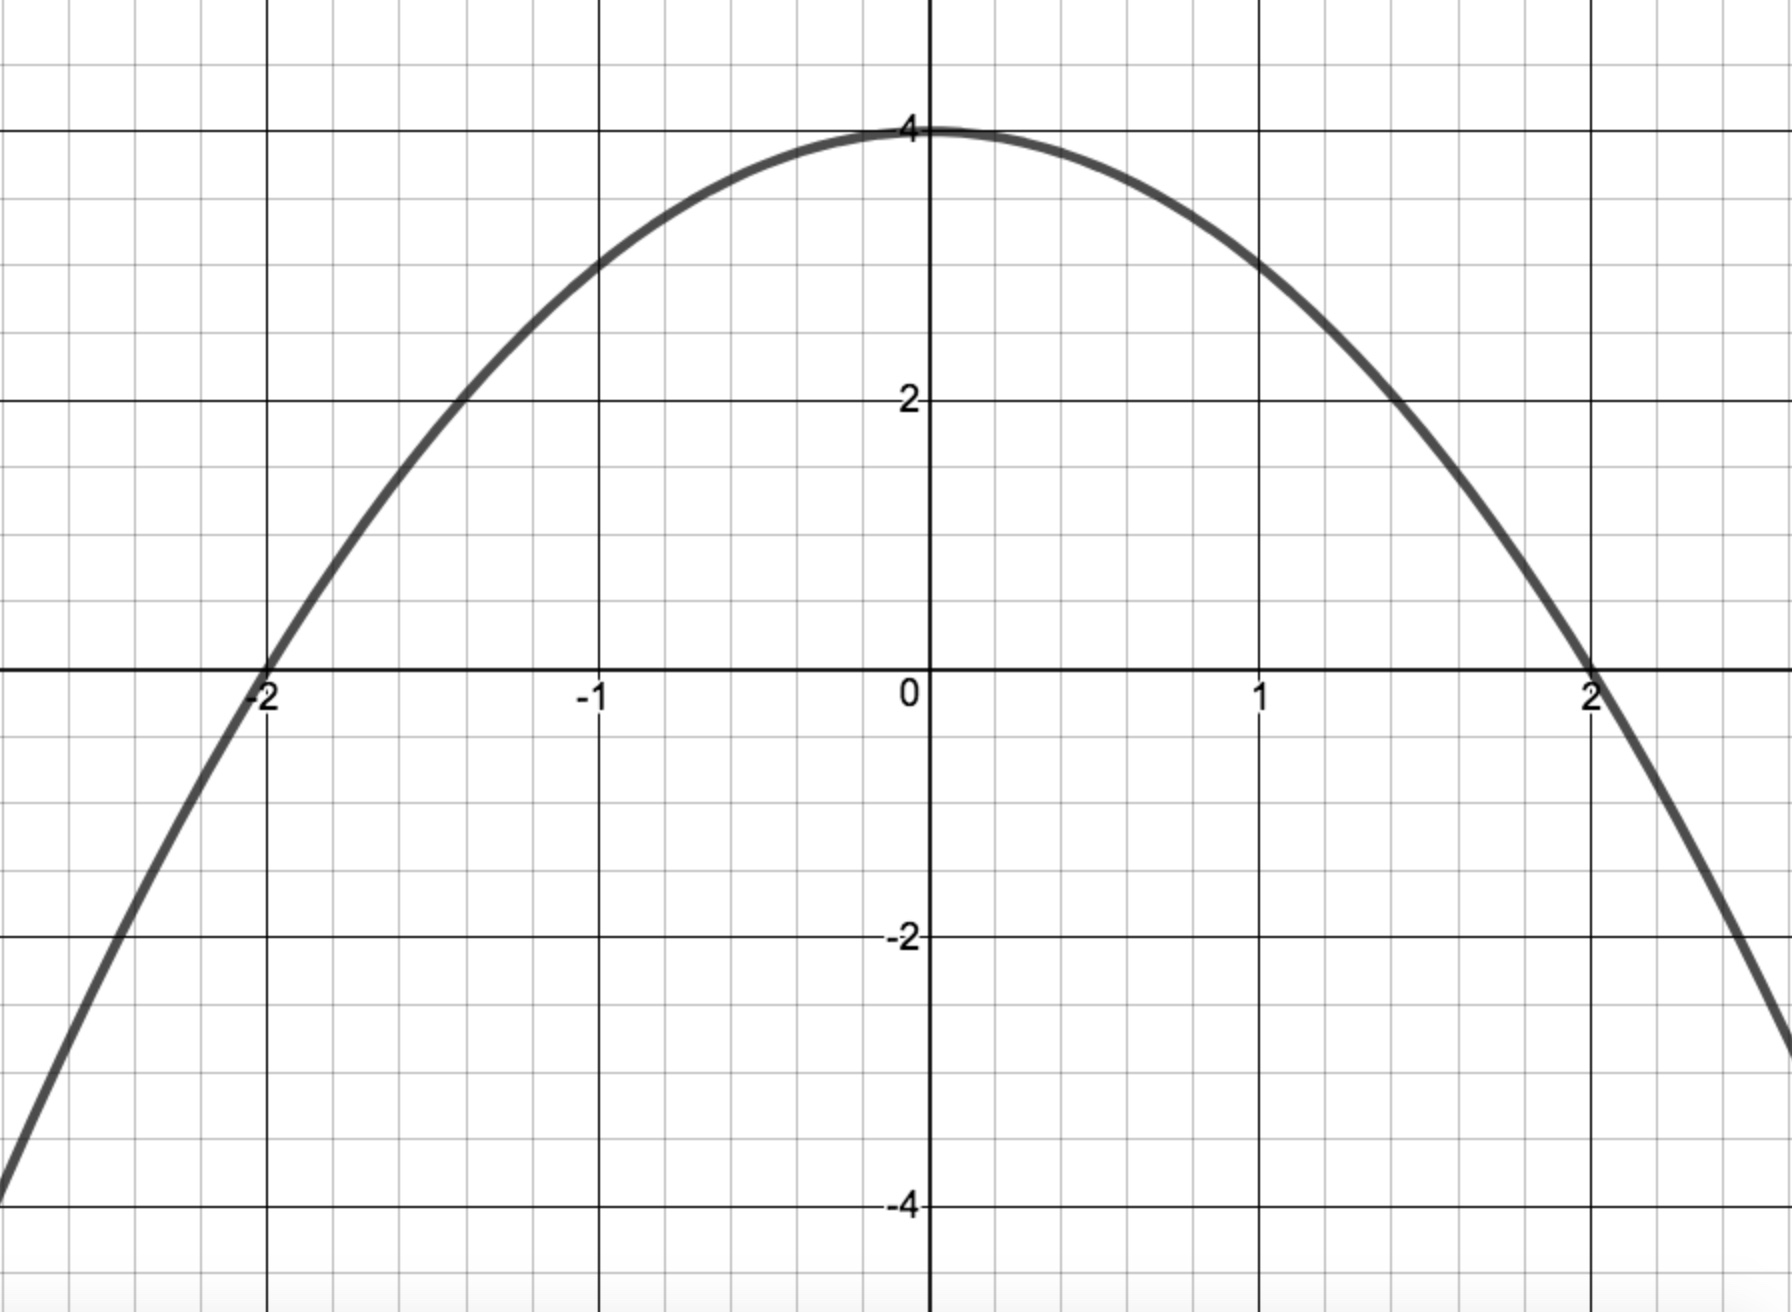
\includegraphics[width=2.75in]{./IntroductiontoDerivativesGraphics/MatchFunc01.jpeg}

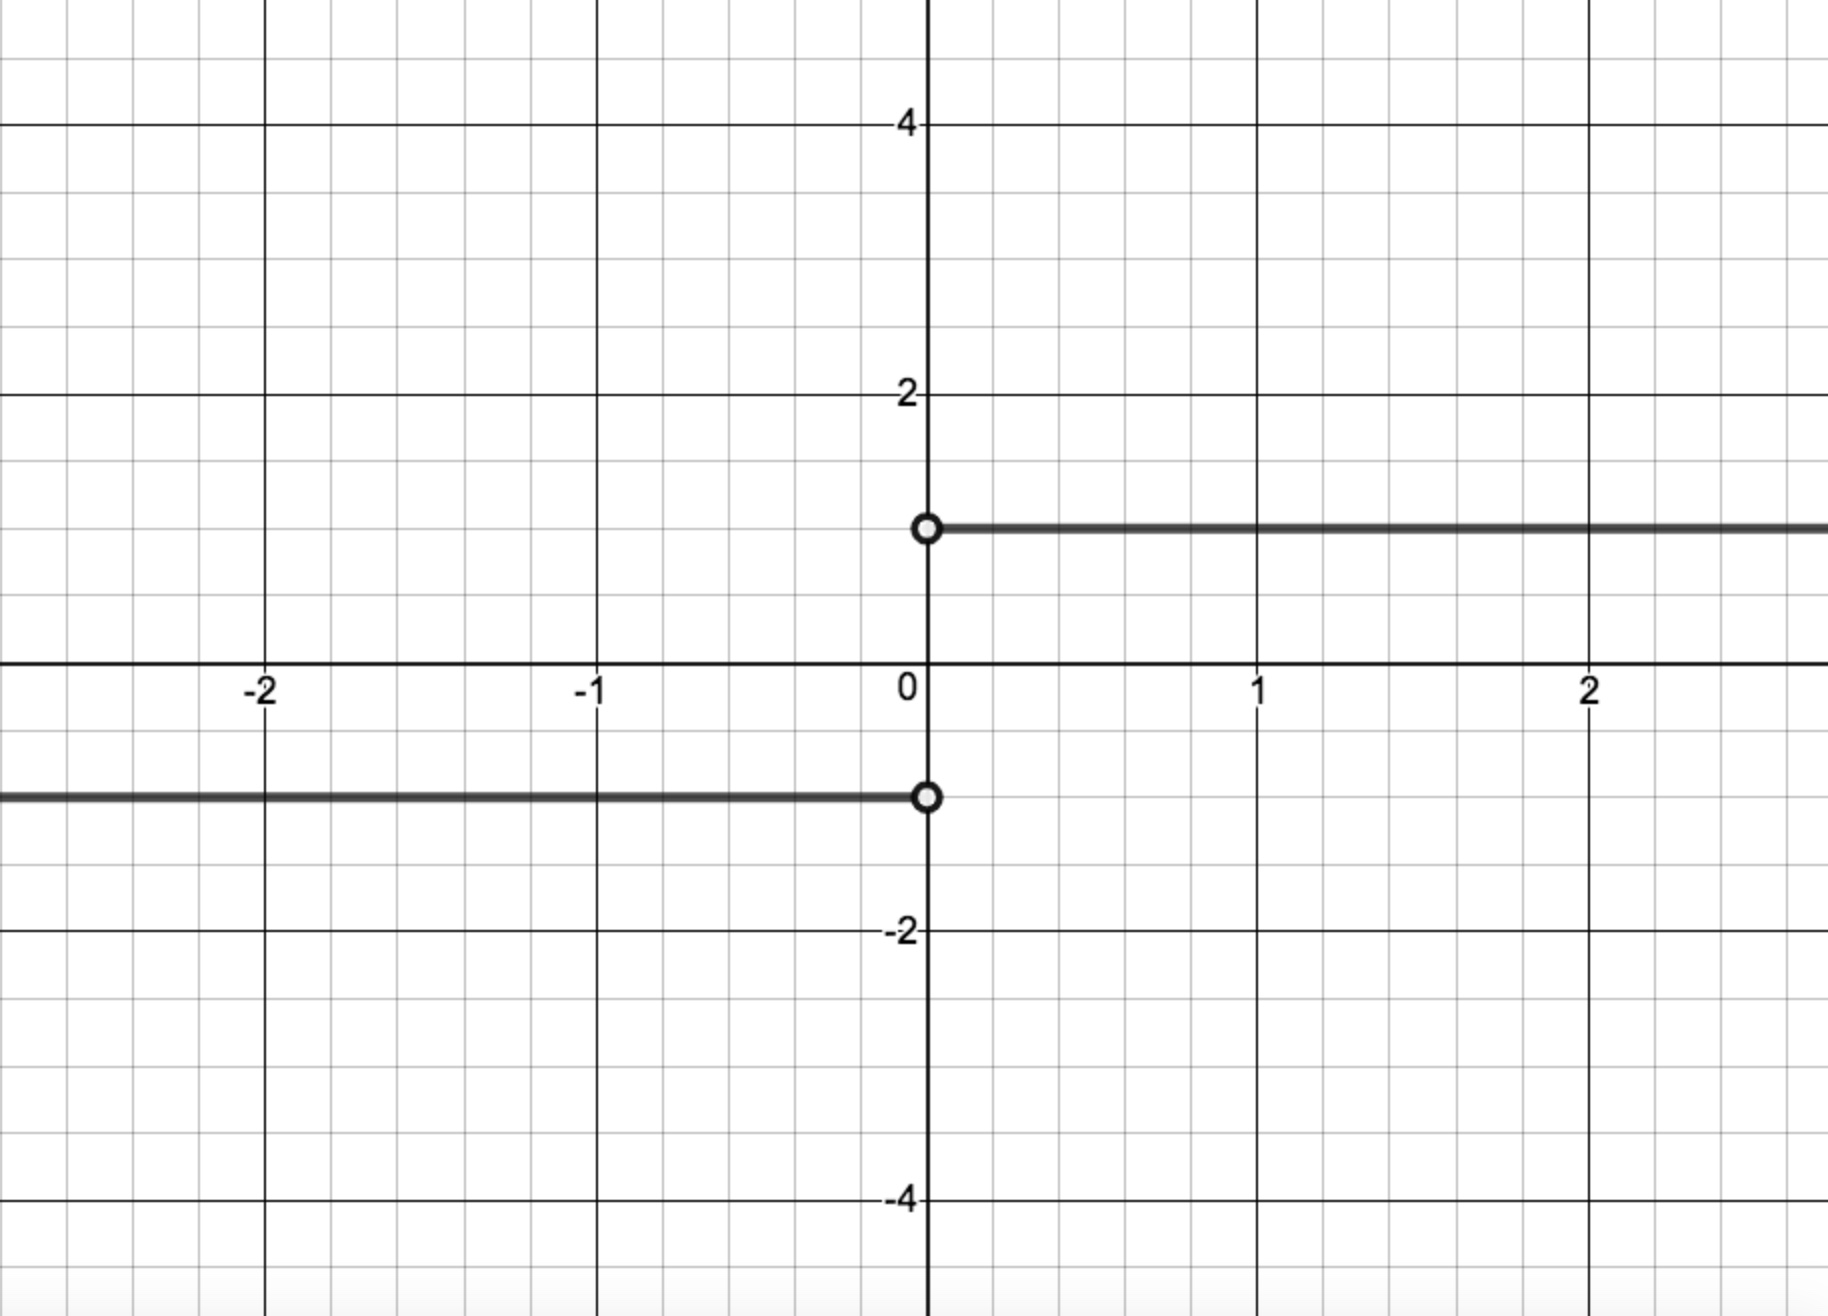
\includegraphics[width=2.75in]{./IntroductiontoDerivativesGraphics/MatchDeriv03.jpeg}

\end{multicols}



\begin{multicols}{2}

\begin{enumerate}
\setcounter{enumi}{\value{HW}}

\item $y = g(x)$:

\setcounter{HW}{\value{enumi}}
\end{enumerate}

Graph B:

\end{multicols}

\begin{multicols}{2}

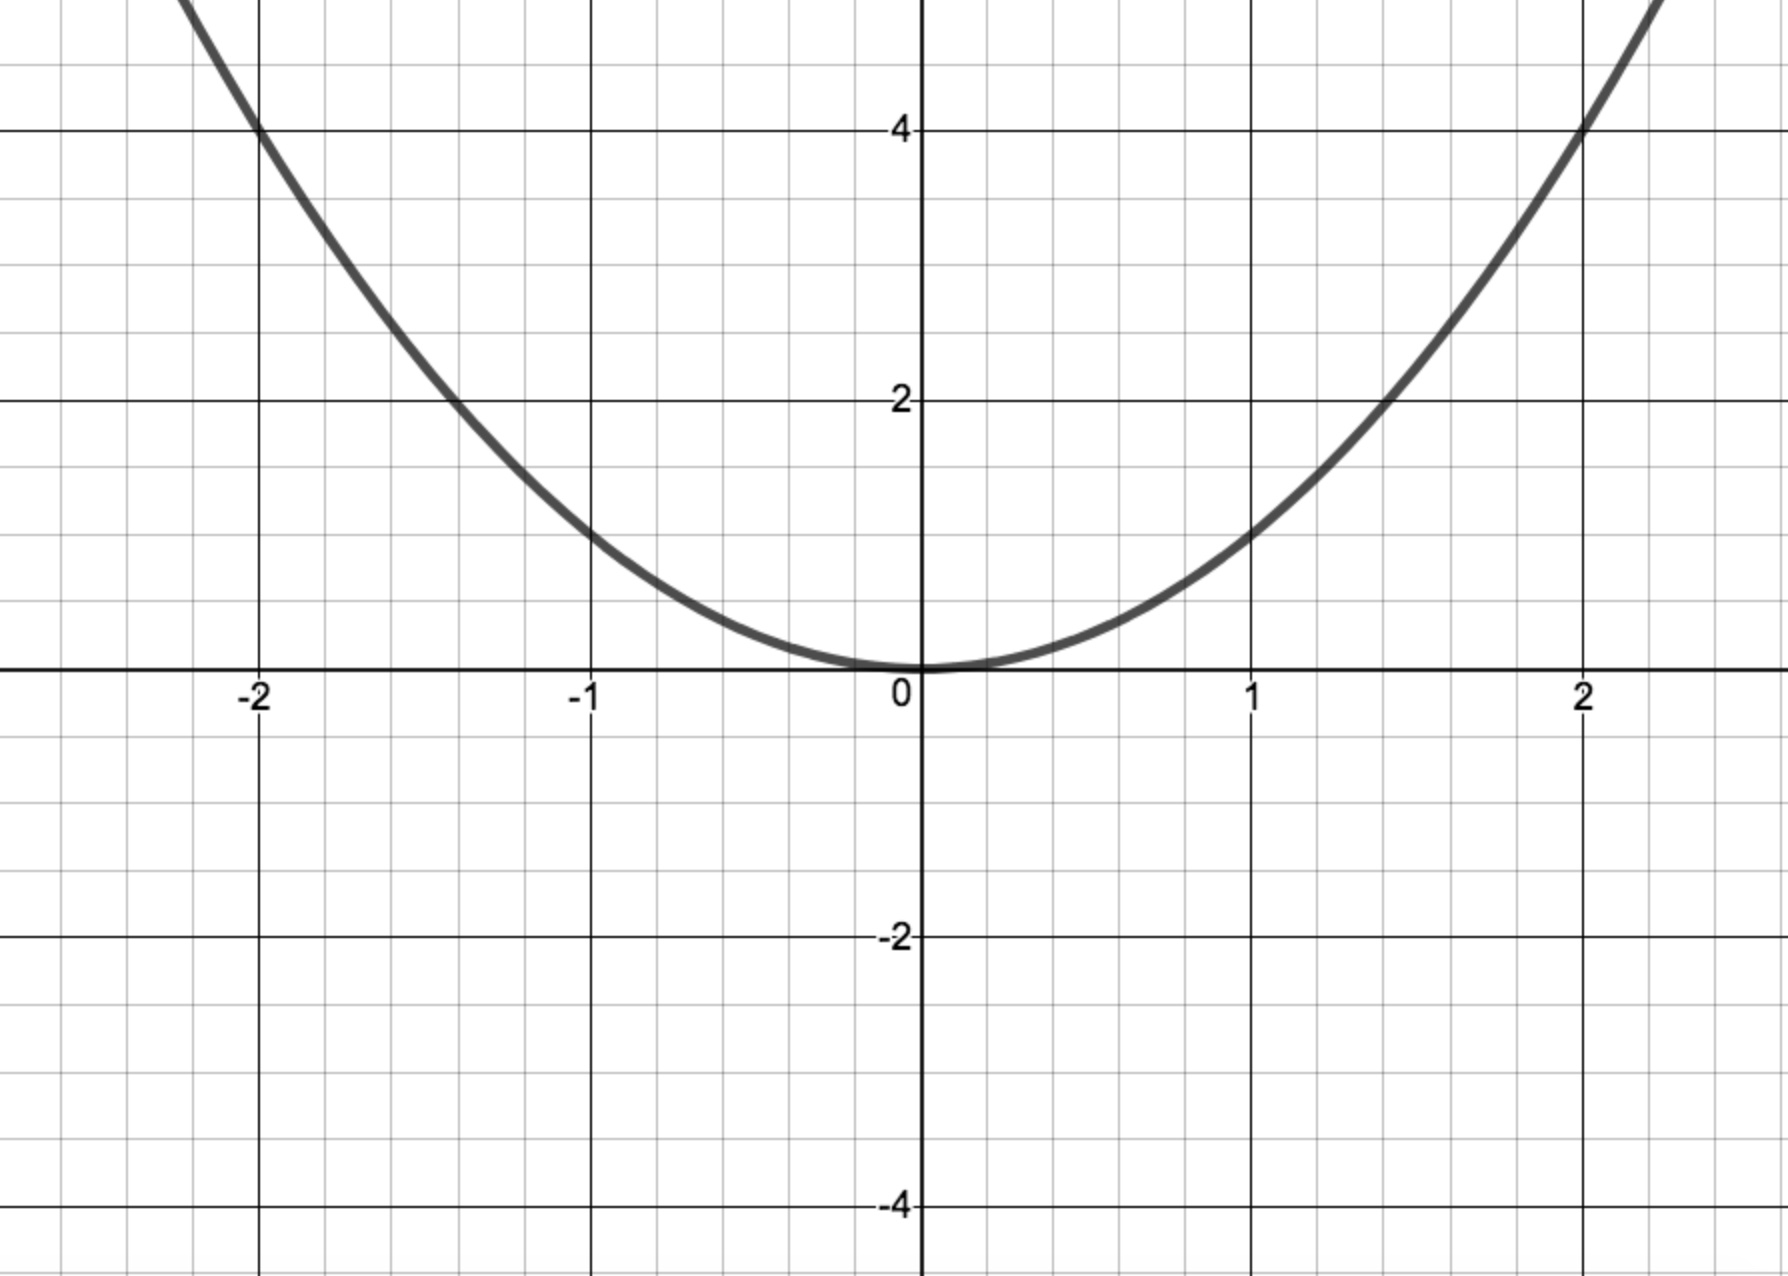
\includegraphics[width=2.75in]{./IntroductiontoDerivativesGraphics/MatchFunc02.jpeg}

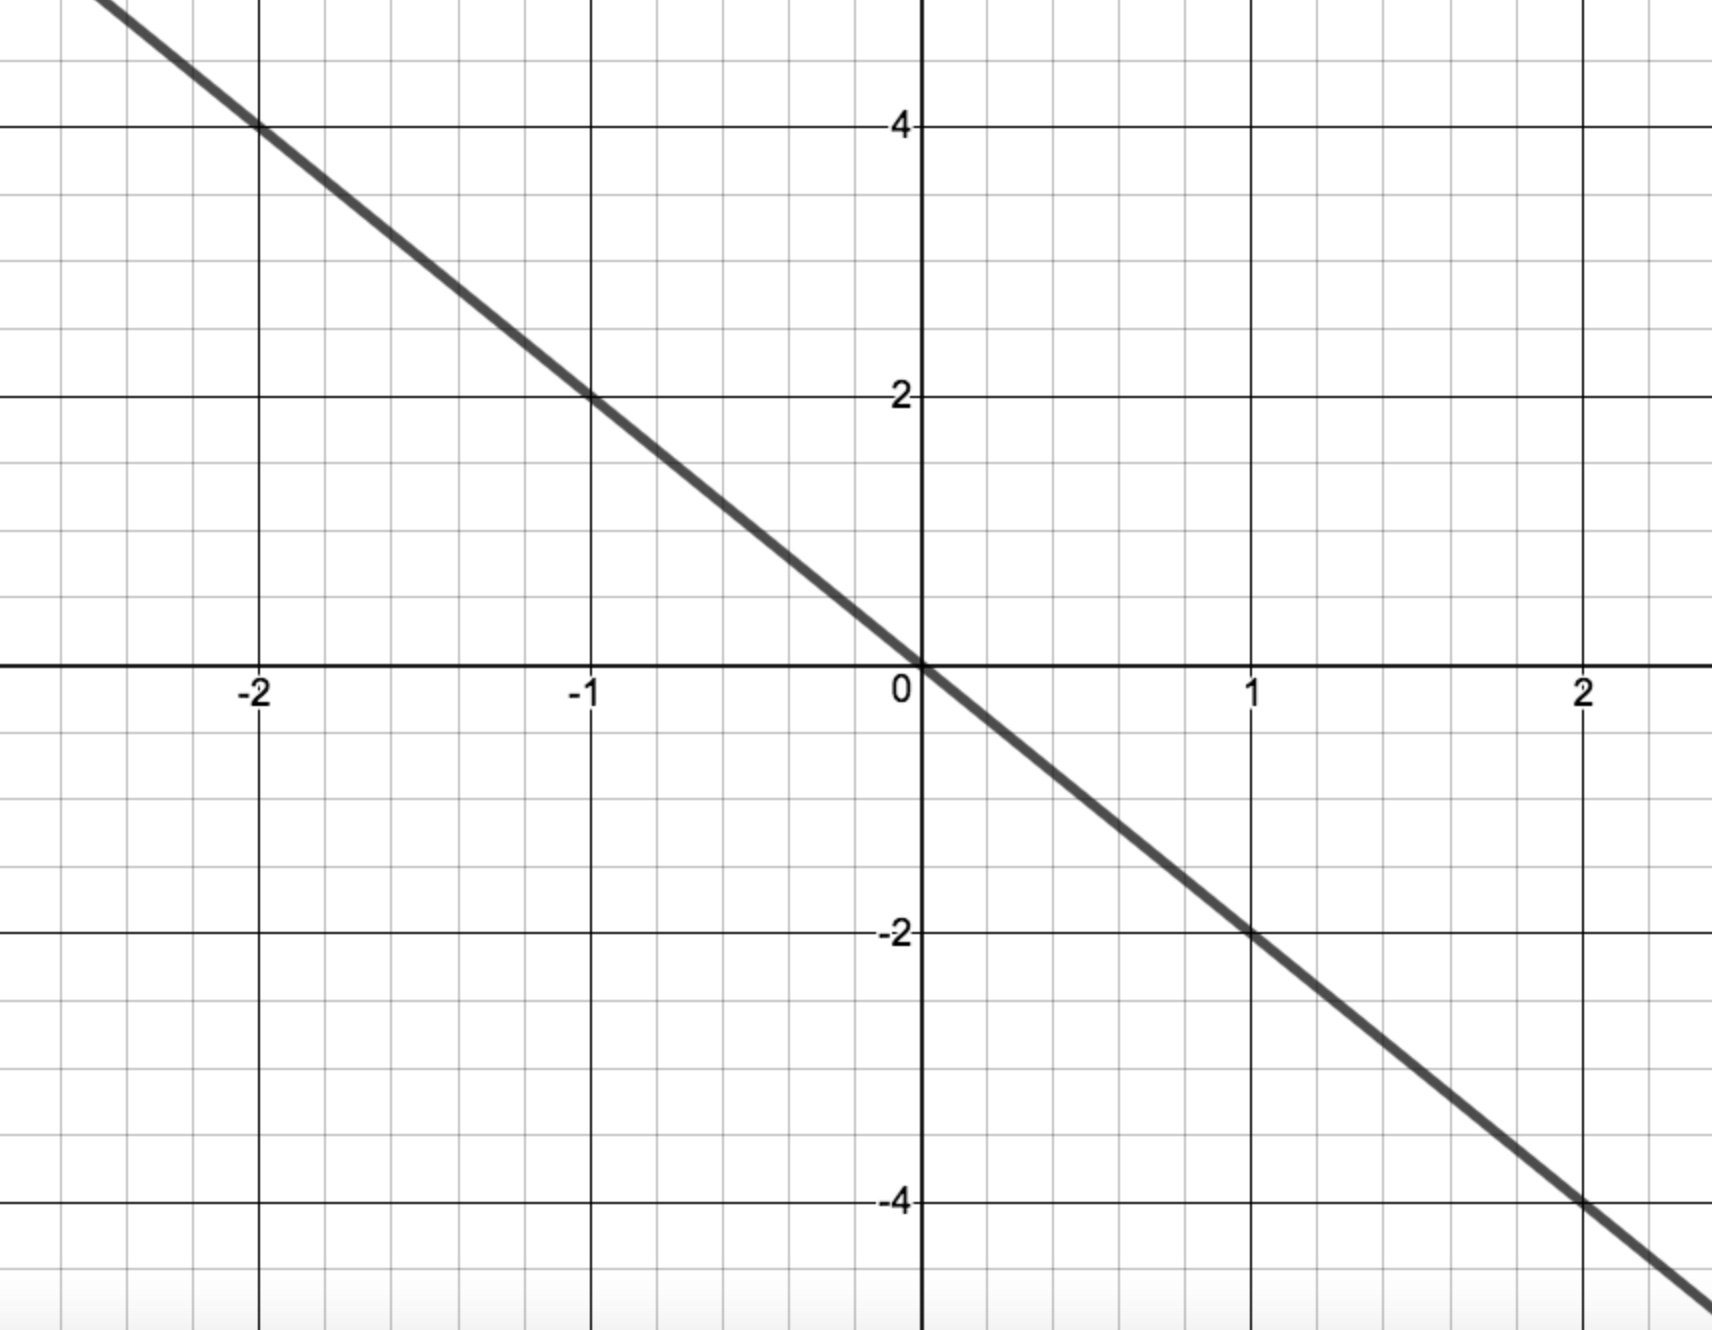
\includegraphics[width=2.75in]{./IntroductiontoDerivativesGraphics/MatchDeriv01.jpeg}

\end{multicols}


\begin{multicols}{2}

\begin{enumerate}
\setcounter{enumi}{\value{HW}}

\item \label{MatchFcnDerivative1last} $y = h(x)$:

\setcounter{HW}{\value{enumi}}
\end{enumerate}


Graph C:

\end{multicols}




\begin{multicols}{2}

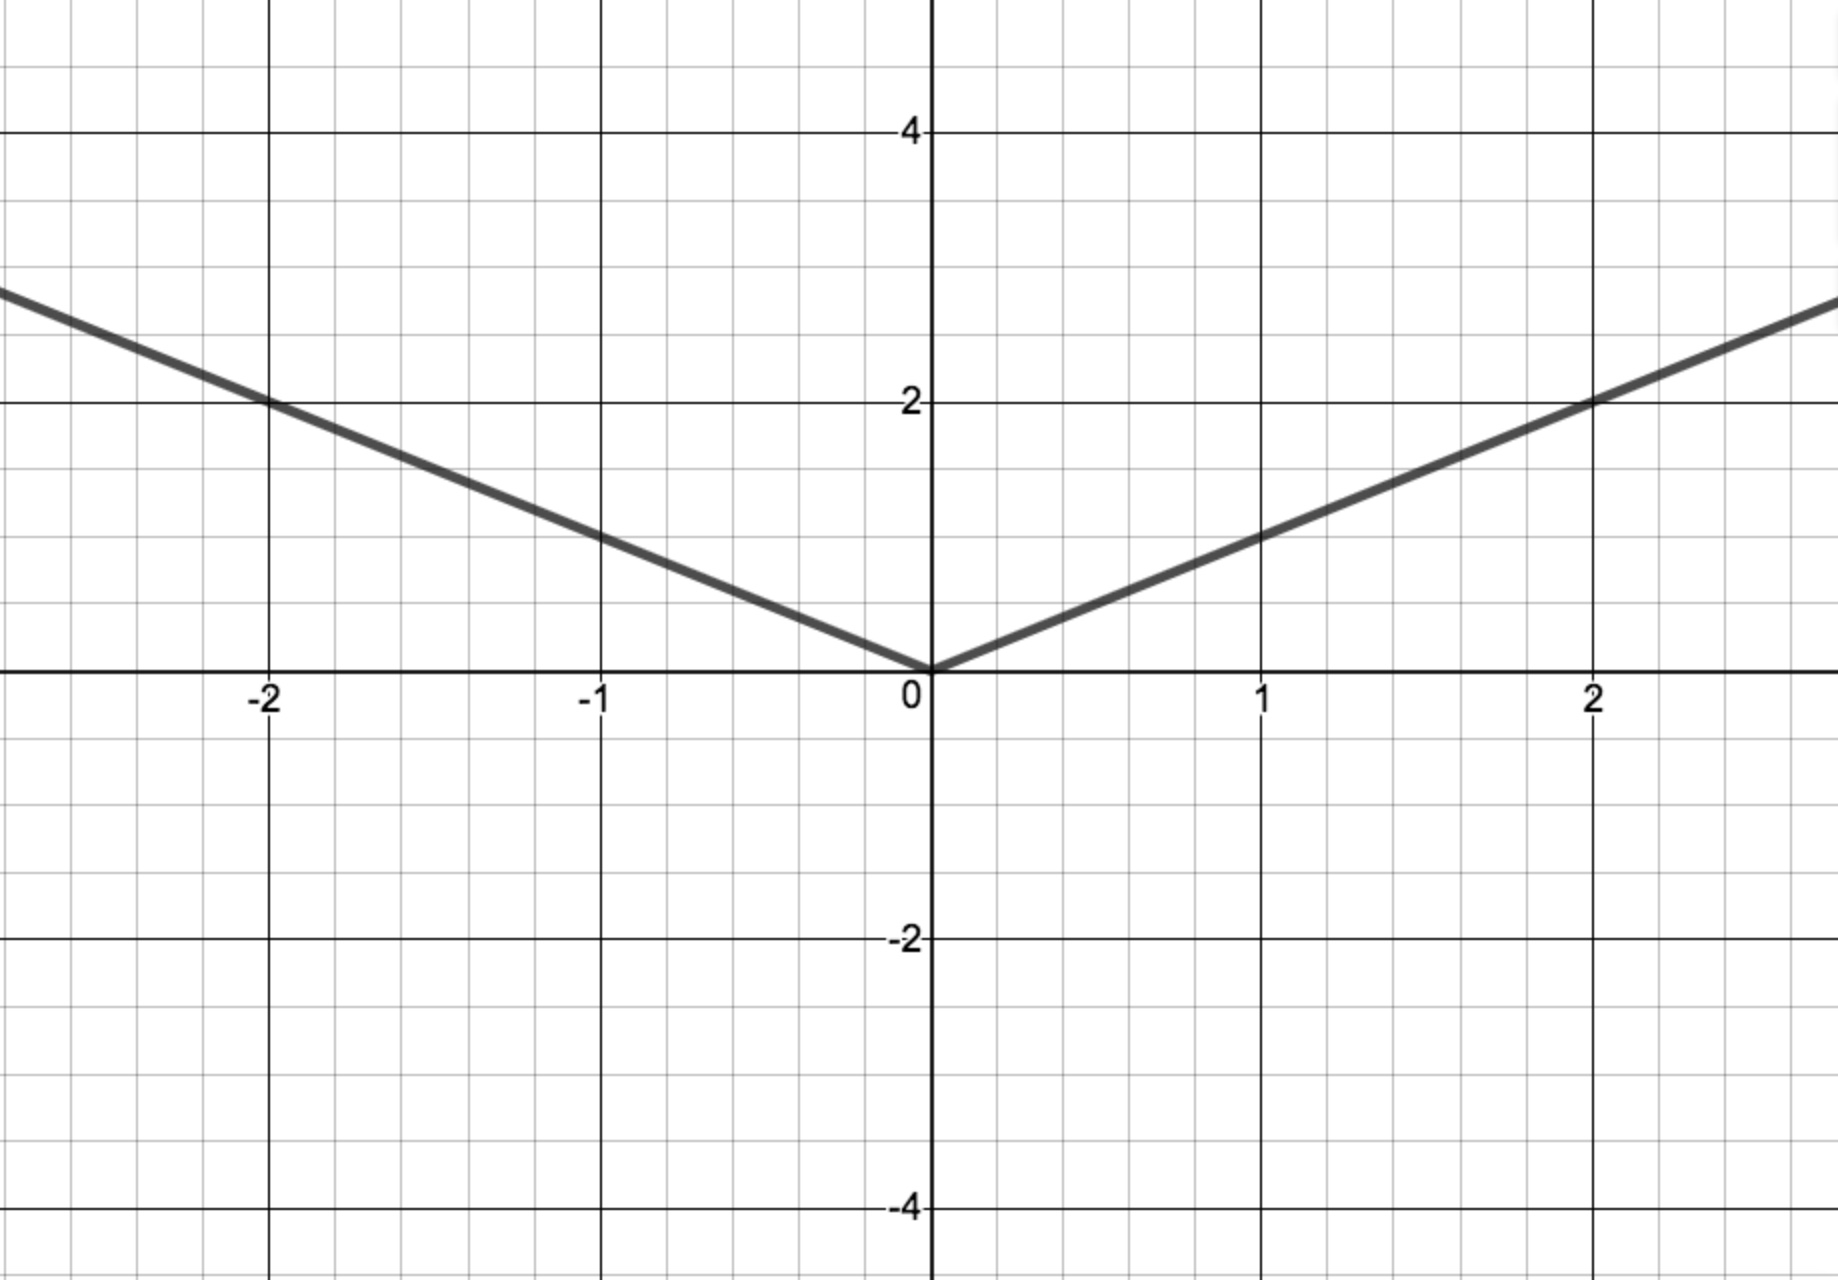
\includegraphics[width=2.75in]{./IntroductiontoDerivativesGraphics/MatchFunc03.jpeg}

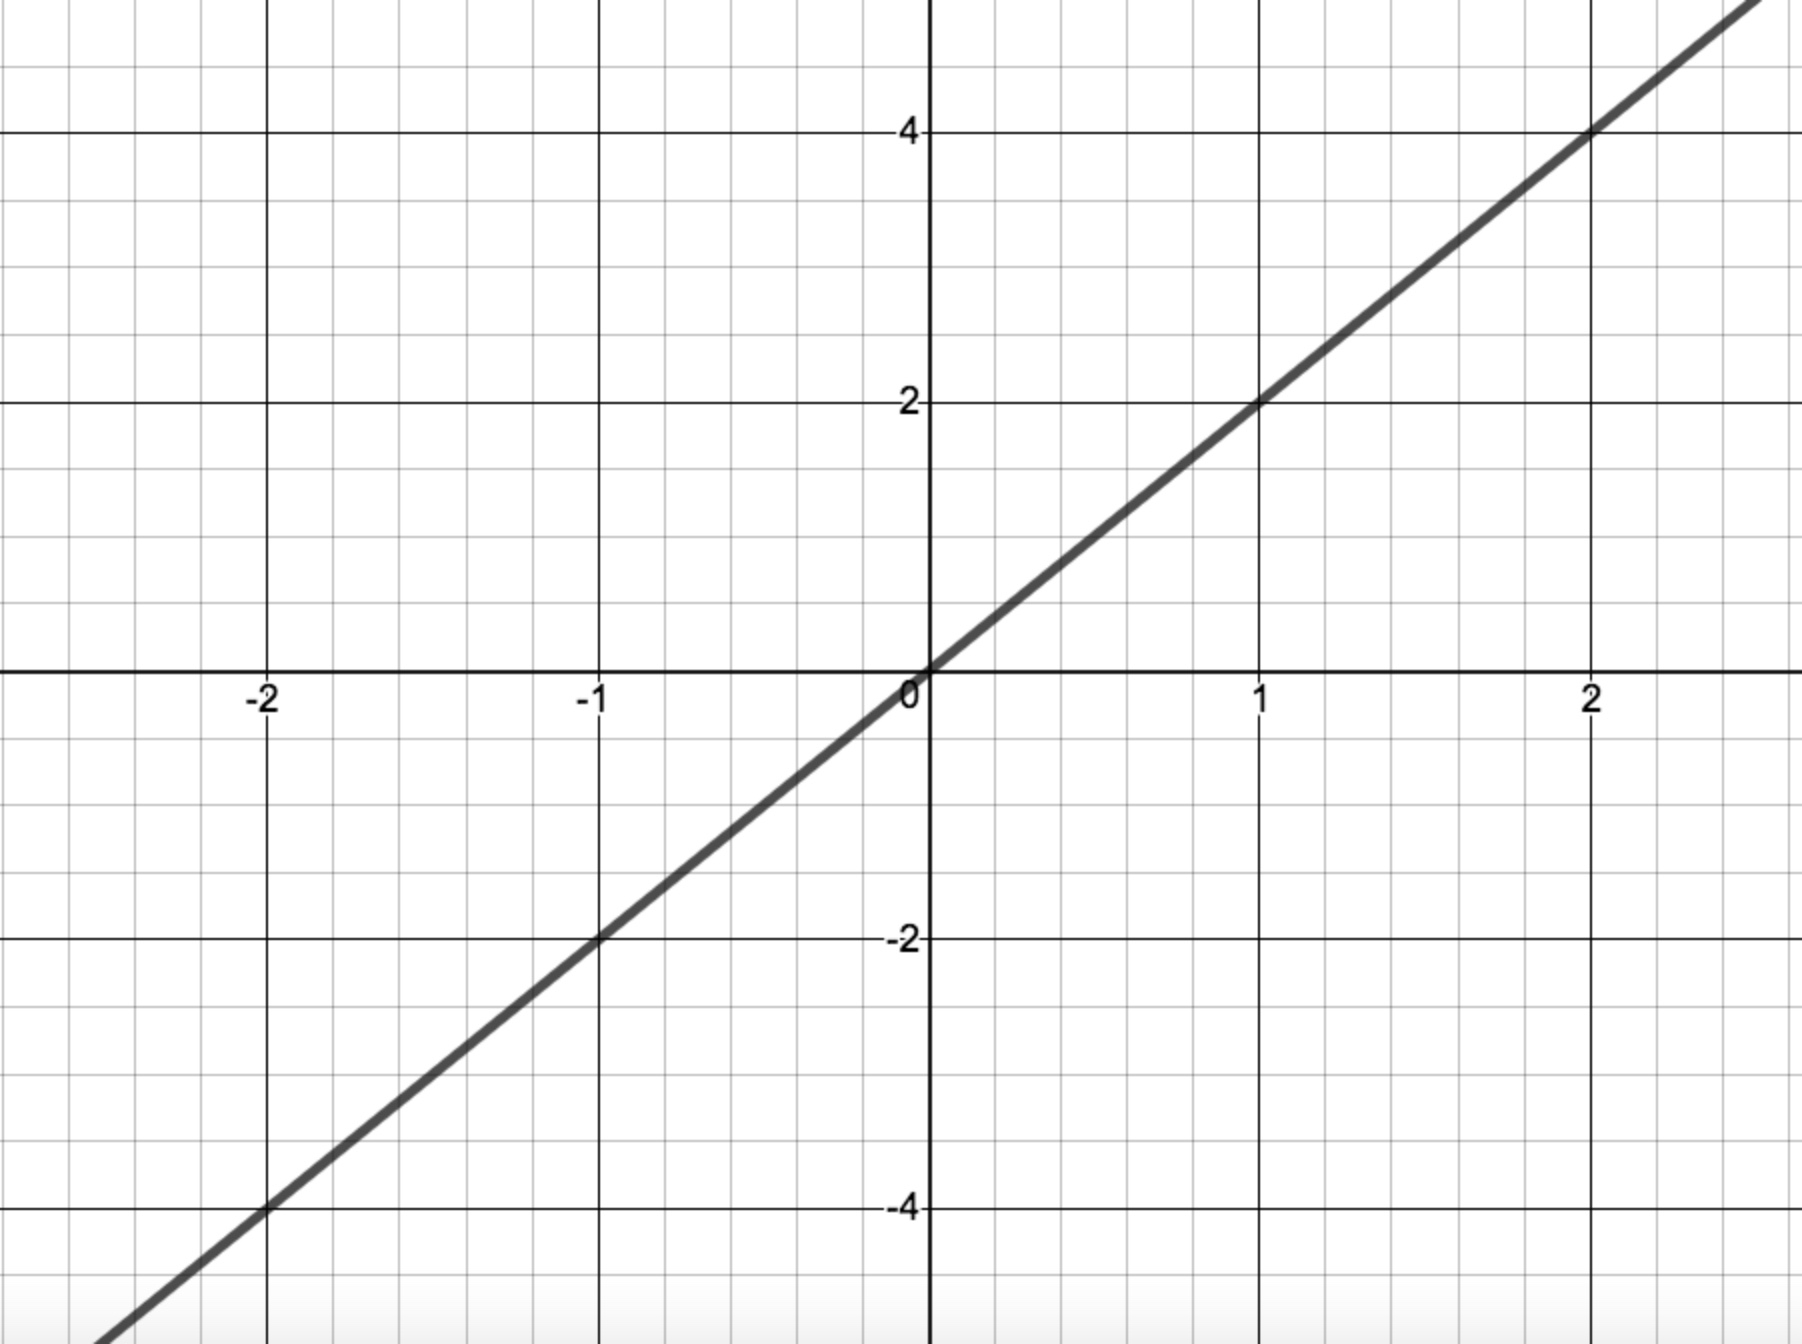
\includegraphics[width=2.75in]{./IntroductiontoDerivativesGraphics/MatchDeriv02.jpeg}

\end{multicols}


\end{center}

In Exercises \ref{MatchFcnDerivative2first} - \ref{MatchFcnDerivative2last}, match the graph of the function with a plausible graph of its derivative.


\begin{center}


\begin{multicols}{2}

\begin{enumerate}
\setcounter{enumi}{\value{HW}}

\item \label{MatchFcnDerivative2first} $y = f(x)$:

\setcounter{HW}{\value{enumi}}
\end{enumerate}

Graph A:

\end{multicols}




\begin{multicols}{2}

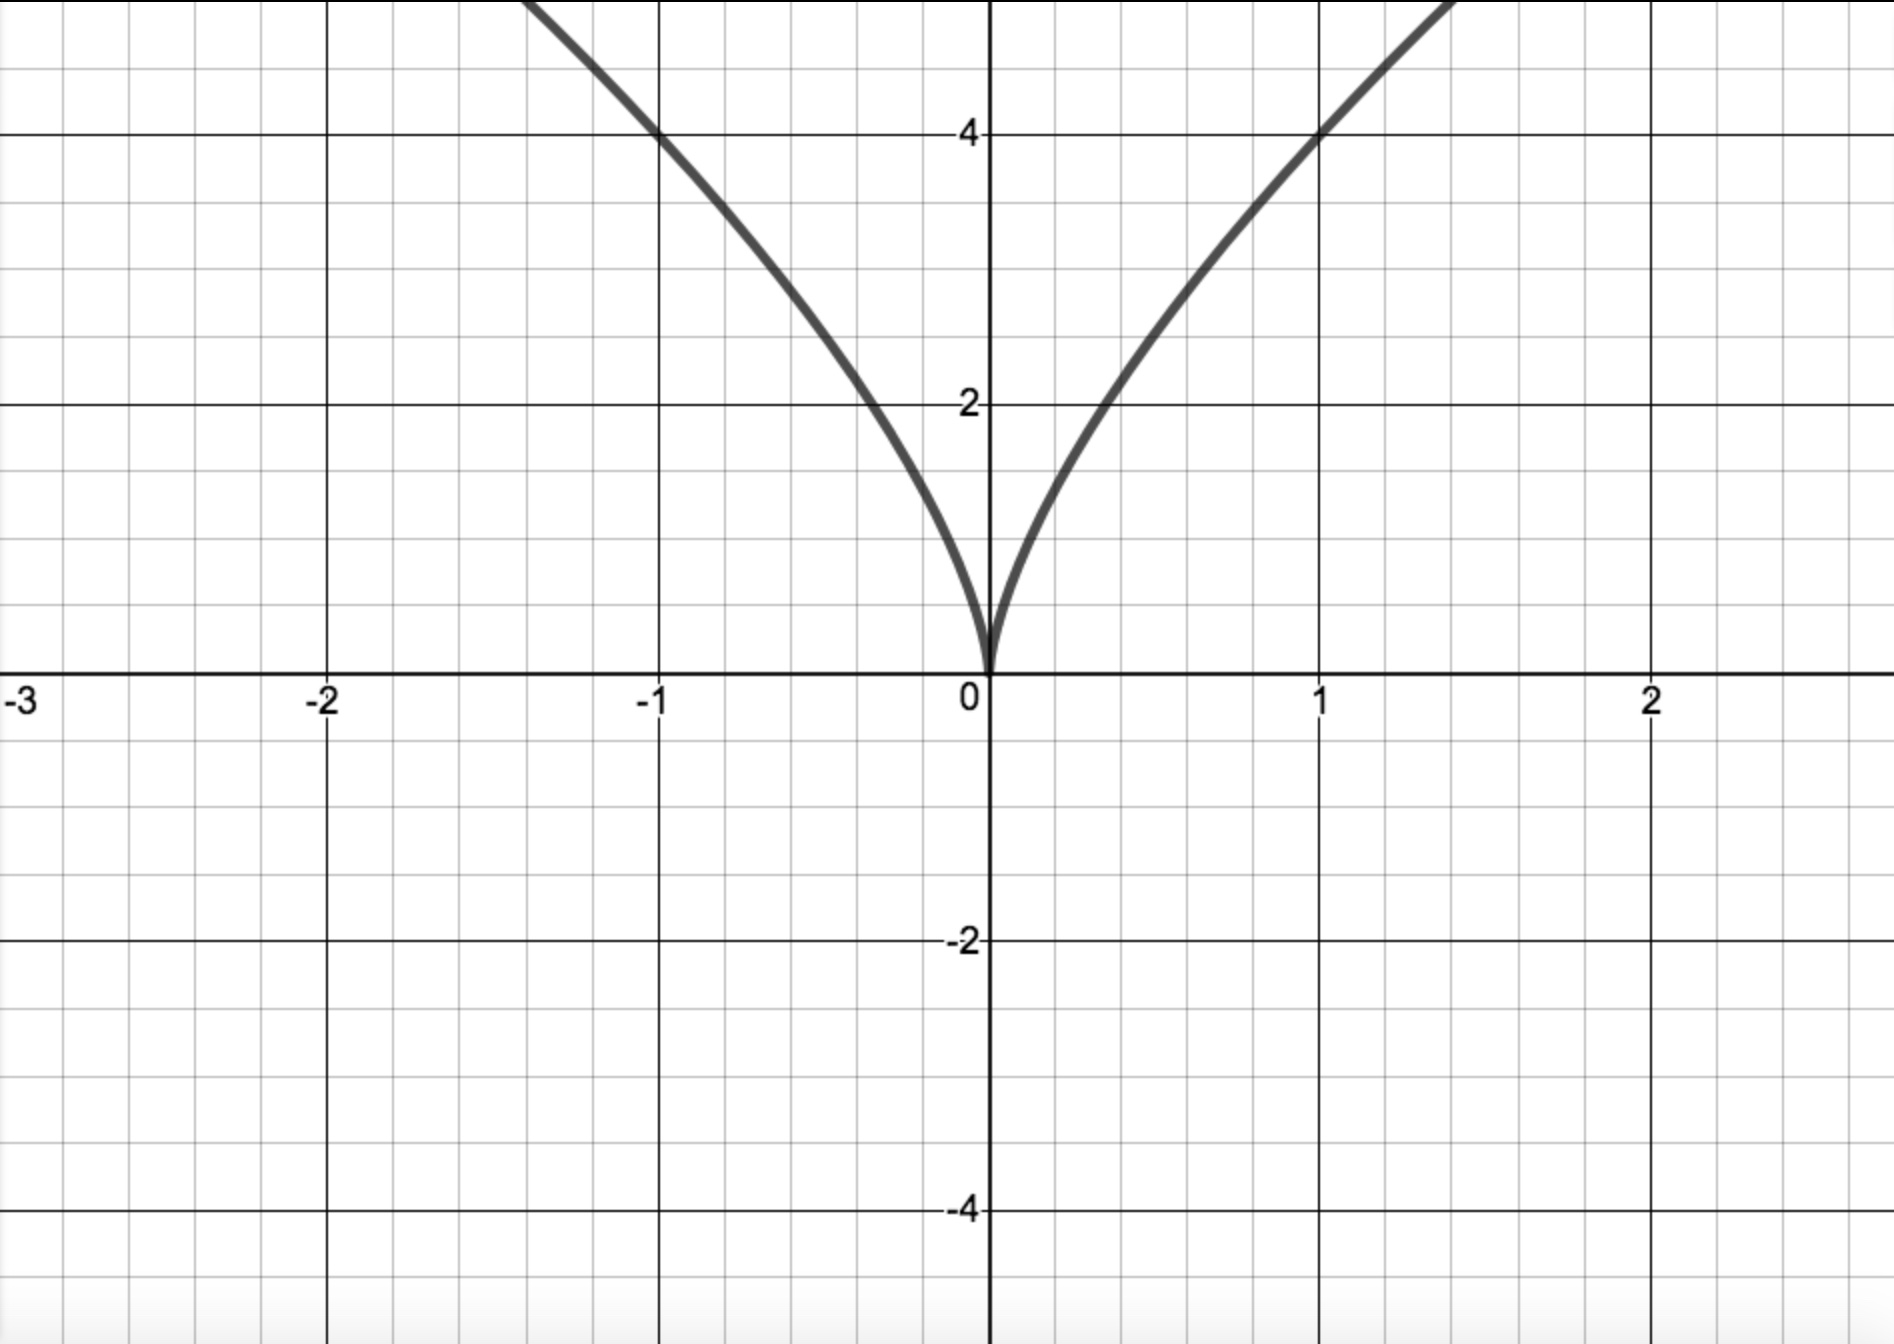
\includegraphics[width=2.75in]{./IntroductiontoDerivativesGraphics/MatchFunc04.jpeg}

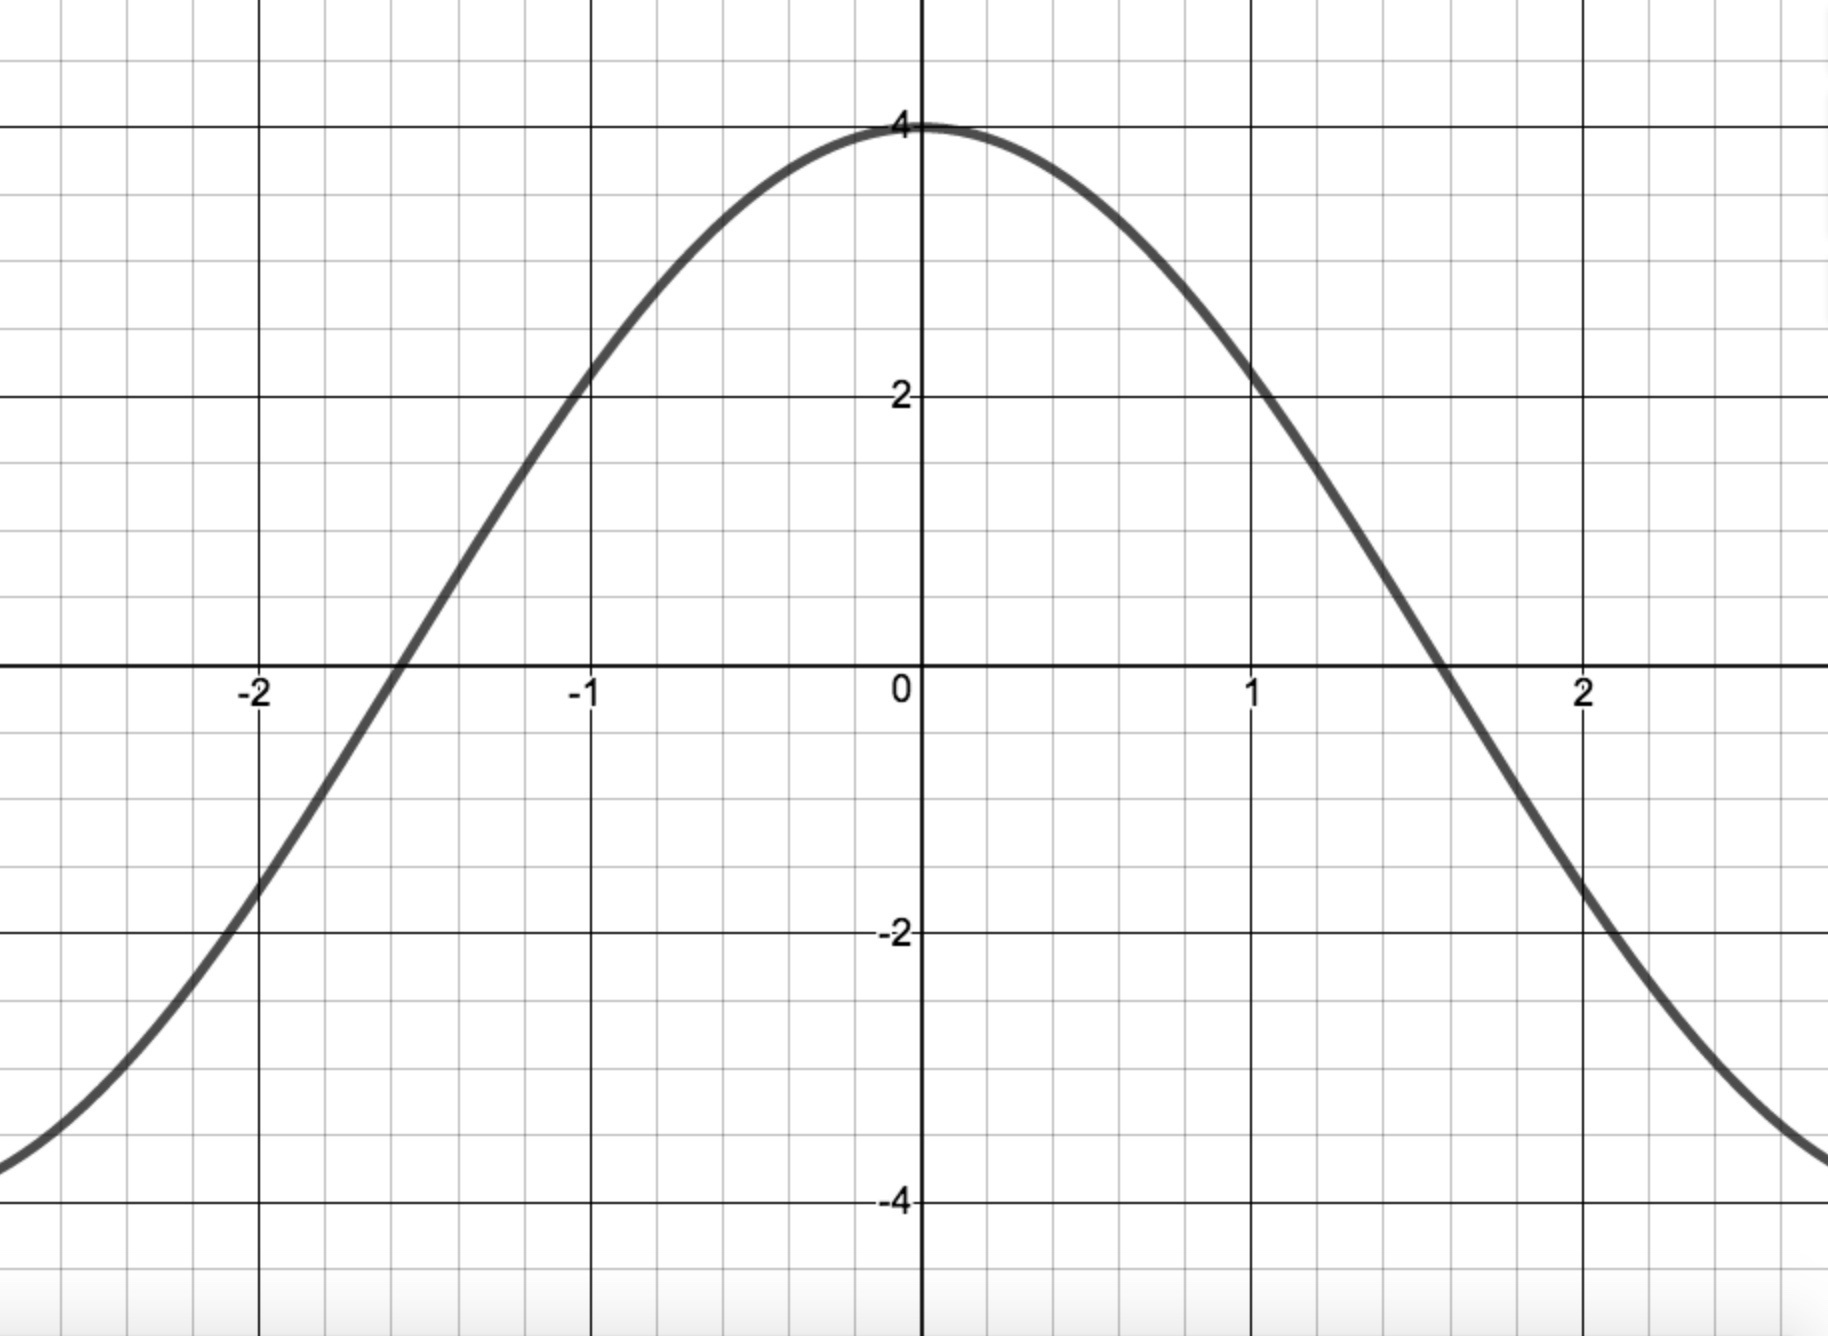
\includegraphics[width=2.75in]{./IntroductiontoDerivativesGraphics/MatchDeriv06.jpeg}

\end{multicols}



\begin{multicols}{2}

\begin{enumerate}
\setcounter{enumi}{\value{HW}}

\item $y = g(x)$:

\setcounter{HW}{\value{enumi}}
\end{enumerate}

Graph B:

\end{multicols}




\begin{multicols}{2}

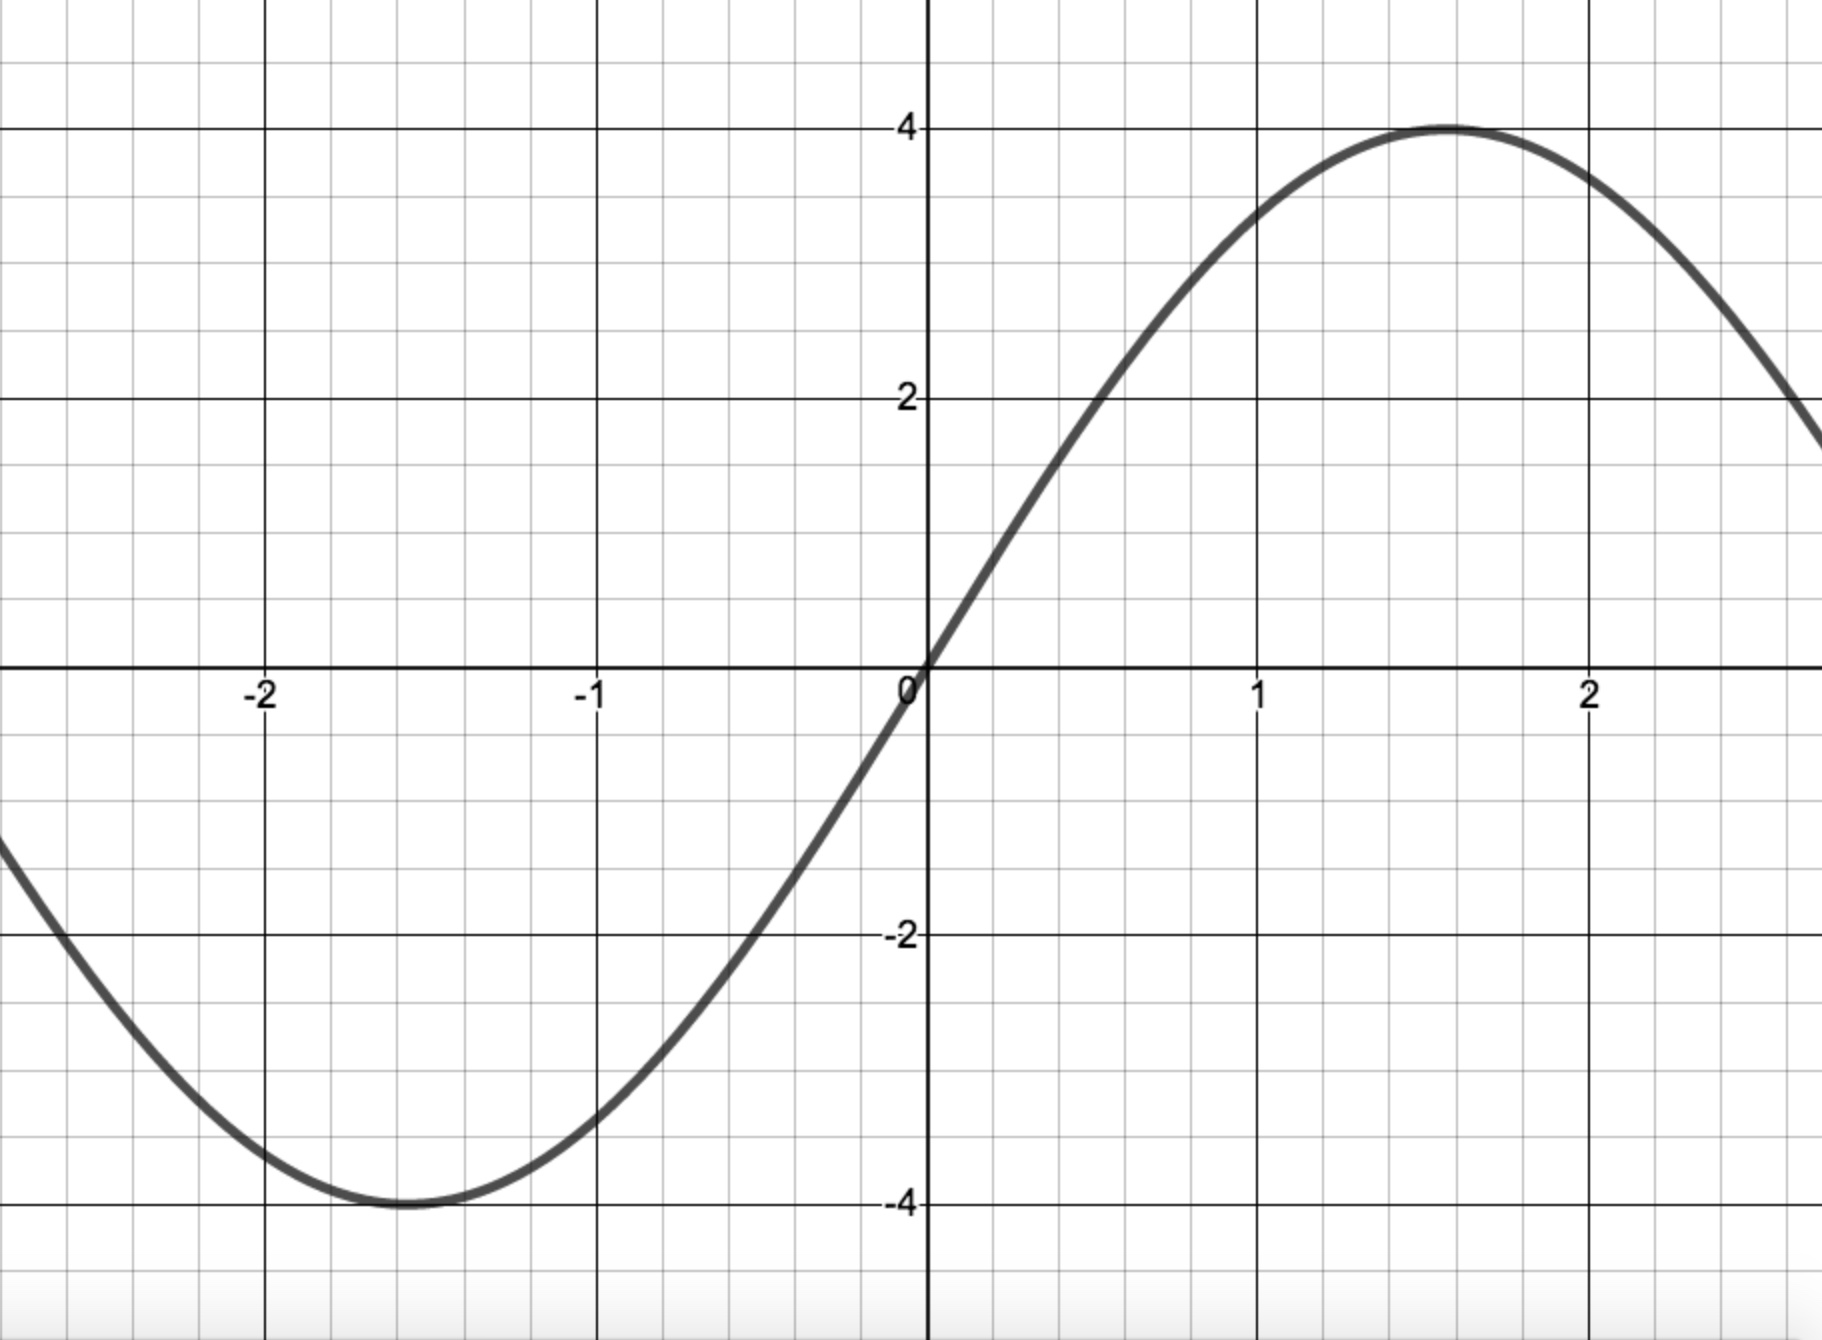
\includegraphics[width=2.75in]{./IntroductiontoDerivativesGraphics/MatchFunc06.jpeg}

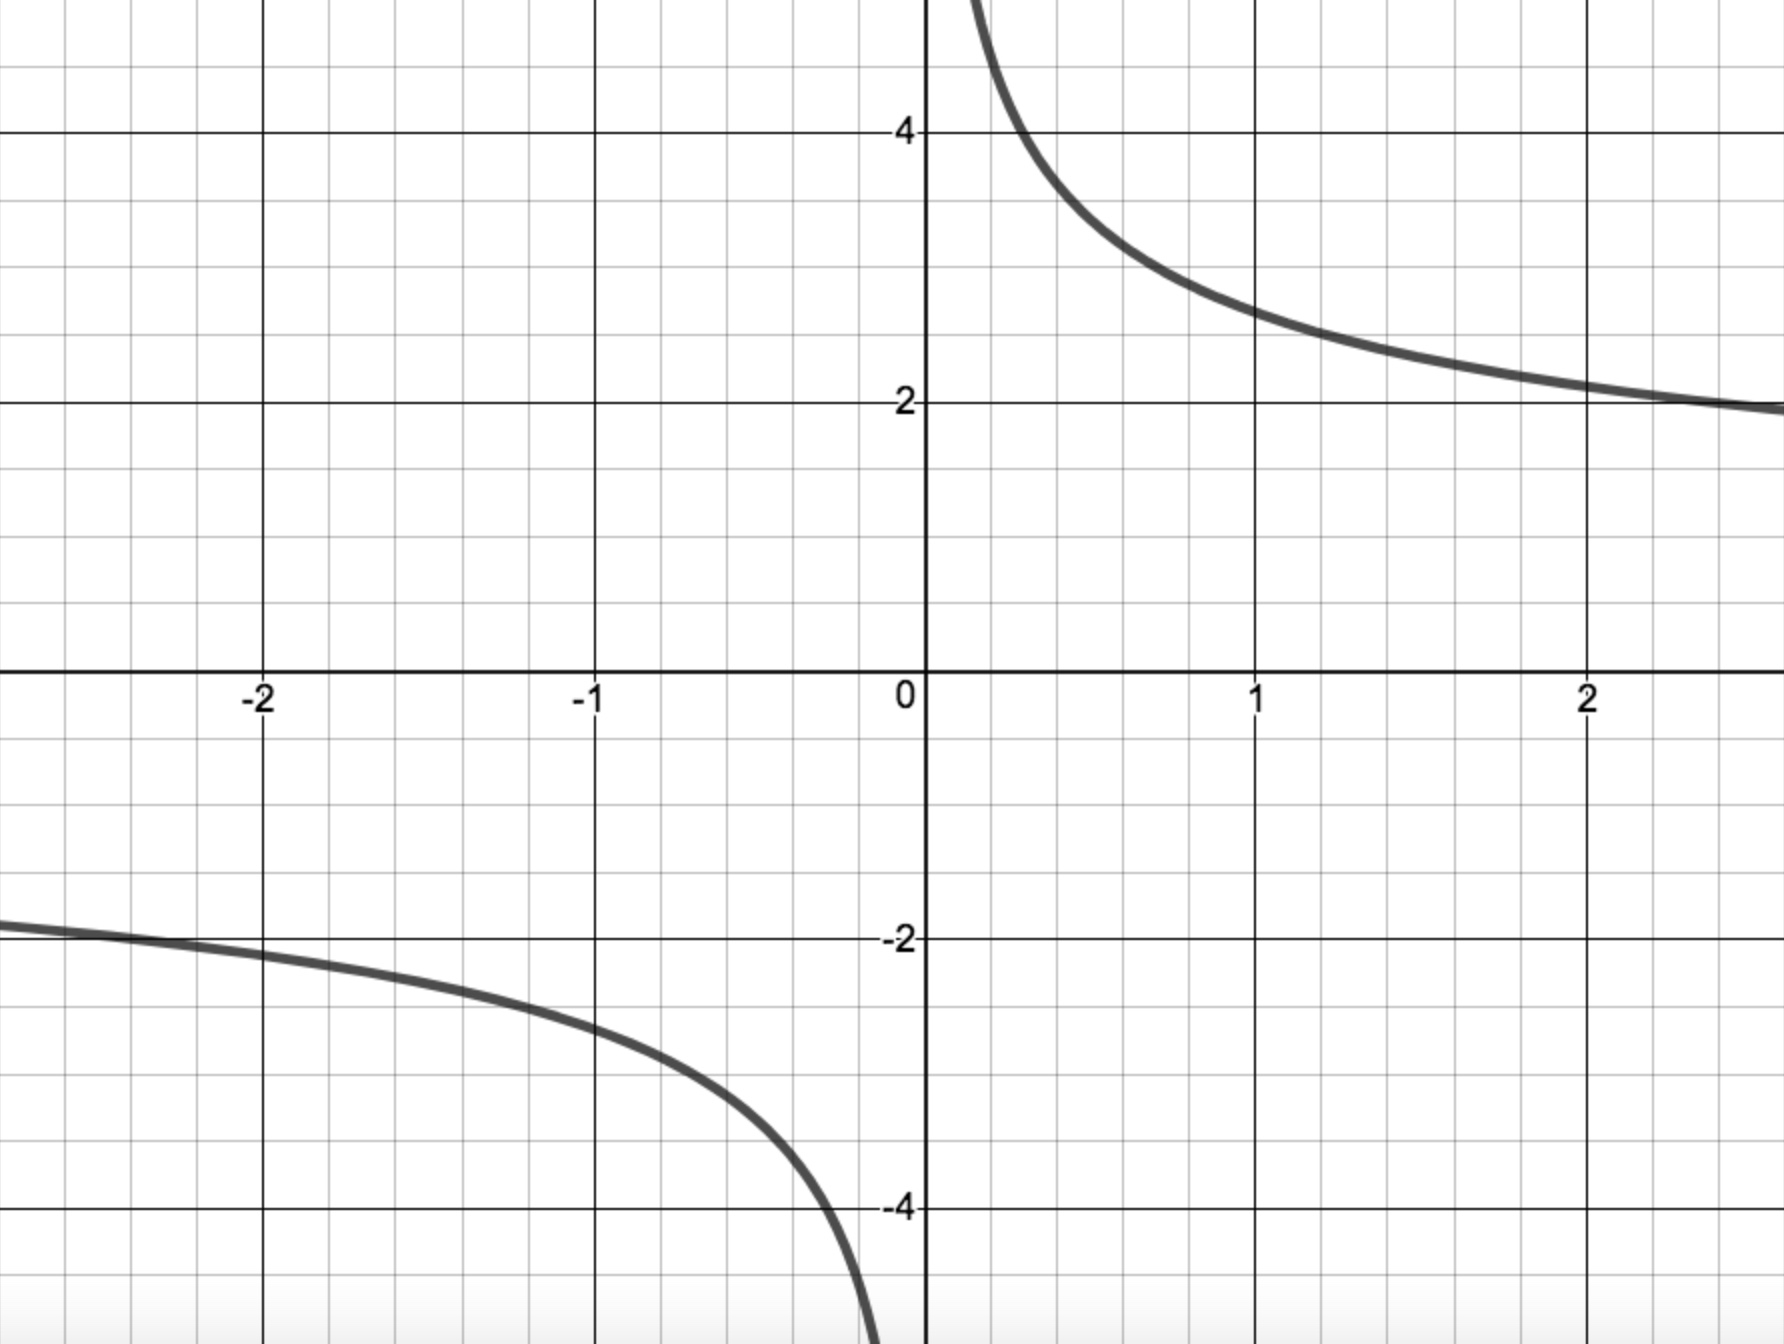
\includegraphics[width=2.75in]{./IntroductiontoDerivativesGraphics/MatchDeriv04.jpeg}

\end{multicols}



\begin{multicols}{2}

\begin{enumerate}
\setcounter{enumi}{\value{HW}}

\item \label{MatchFcnDerivative2last}  $y = h(x)$:

\setcounter{HW}{\value{enumi}}
\end{enumerate}

Graph C:

\end{multicols}



\begin{multicols}{2}

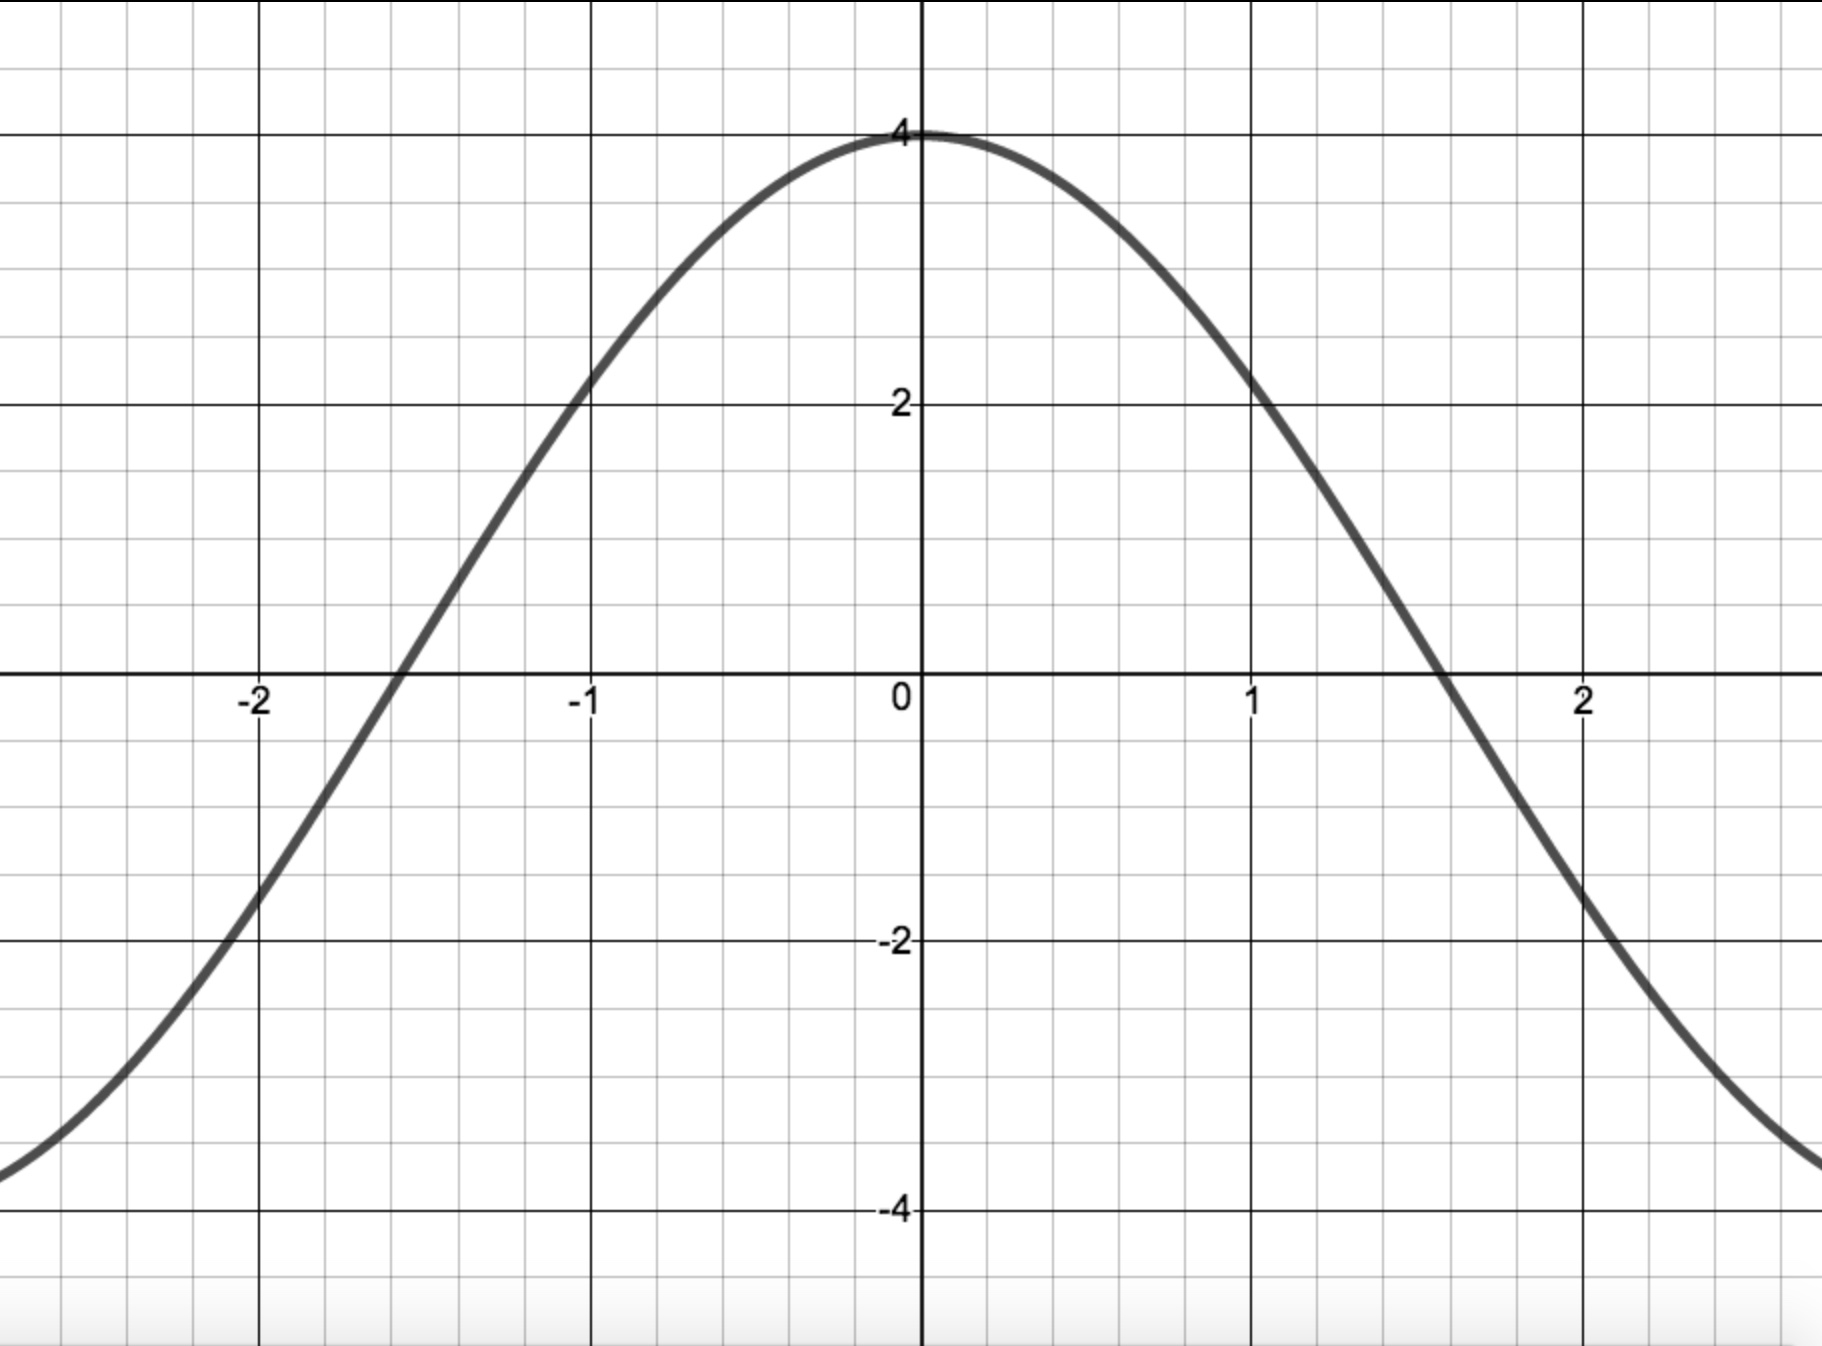
\includegraphics[width=2.75in]{./IntroductiontoDerivativesGraphics/MatchFunc05.jpeg}

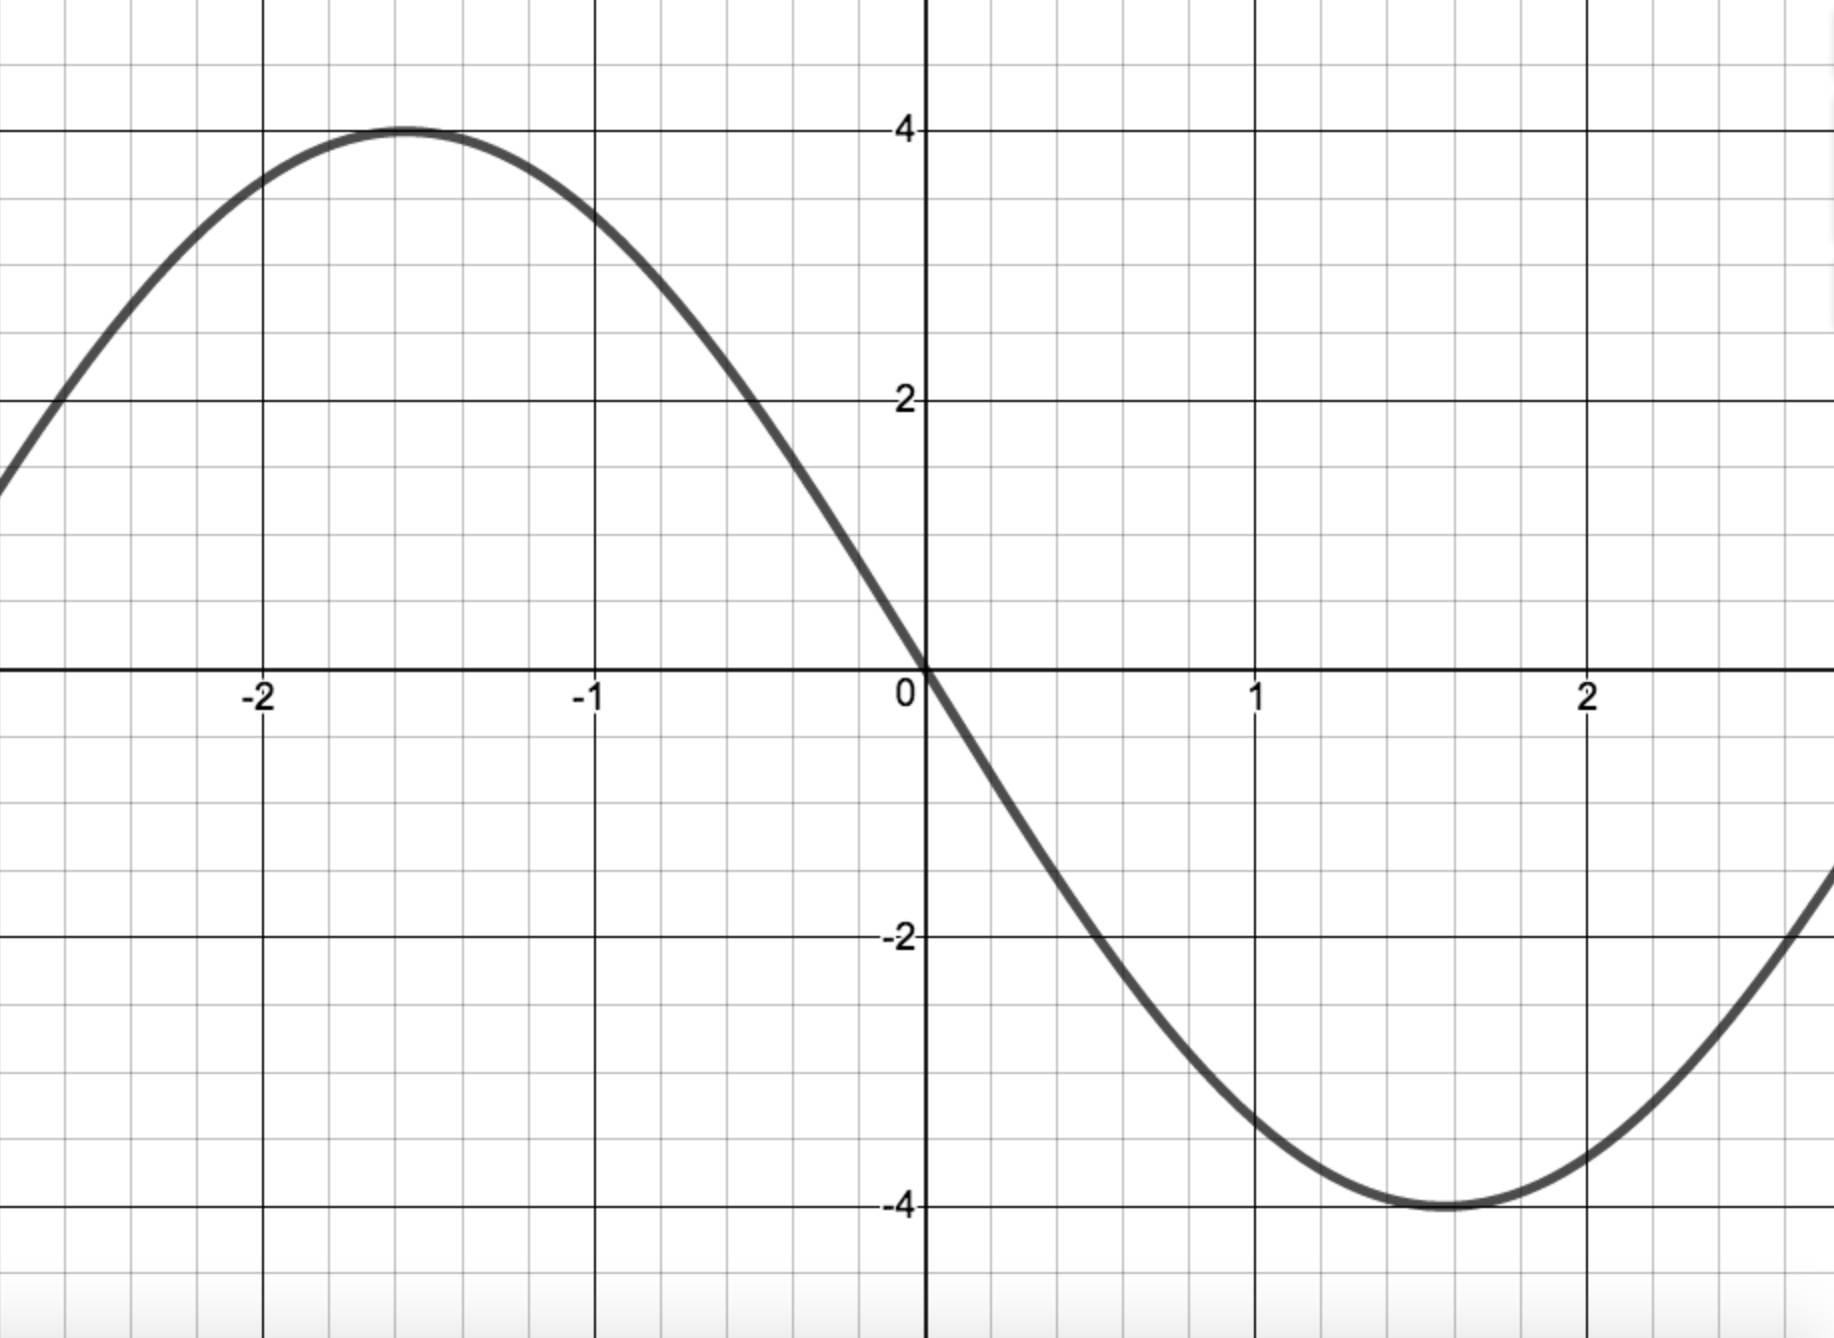
\includegraphics[width=2.75in]{./IntroductiontoDerivativesGraphics/MatchDeriv05.jpeg}

\end{multicols}

\end{center}


\newpage


\subsection{Answers}


\begin{enumerate}

\item $\ds{\lim_{h \rightarrow 0} 2 = 2}$, $\ds{\lim_{h \rightarrow 0} 2 = 2}$
\item $\ds{\lim_{h \rightarrow 0} -3 = -3}$, $\ds{\lim_{h \rightarrow 0} -3 = -3}$,

\setcounter{HW}{\value{enumi}}
\end{enumerate}

\begin{enumerate}
\setcounter{enumi}{\value{HW}}

\item $\ds{\lim_{h \rightarrow 0} 0 = 0}$,  $\ds{\lim_{h \rightarrow 0} 0 = 0}$
\item  $\ds{\lim_{h \rightarrow 0} (3h+11)= 11}$,   $\ds{\lim_{h \rightarrow 0} (6x+3h-1)= 6x-1}$

\setcounter{HW}{\value{enumi}}
\end{enumerate}

\begin{enumerate}
\setcounter{enumi}{\value{HW}}

\item    $\ds{\lim_{h \rightarrow 0} (-h-2) = -2}$,   $\ds{\lim_{h \rightarrow 0} (-2x-h+2) = -2x+2}$   
\item   $\ds{\lim_{h \rightarrow 0} (4h+16) = 16}$,   $\ds{\lim_{h \rightarrow 0} (8x+4h) = 8x}$ 

\setcounter{HW}{\value{enumi}}
\end{enumerate}

\begin{enumerate}
\setcounter{enumi}{\value{HW}}

\item \begin{itemize}  \item $f'(2) = \ds{\lim_{h \rightarrow 0} (-h-3) = -3}$

\smallskip

\item  $y = f'(2)(x-2) + f(2) = (-3)(x-2)+(-2)$ so $y  = -3x+4$.

\smallskip

\item   $f'(x) =  \ds{\lim_{h \rightarrow 0} (-2x-h+1) = -2x+1}$ 

\smallskip

\item  $y = f'(0)(x-0) + f(0) = (1)(x-0) + 0$ so $y = x$.

\smallskip

\end{itemize}

\item \begin{itemize}

\item $f'(2) = \ds{\lim_{h \rightarrow 0} \left( h^2+6h+12 \right) = 12}$

\smallskip

\item  $y = f'(2)(x-2) + f(2) = 12(x-2)+ 9$ so $y = 12x - 15$.

\smallskip

\item  $f'(x) = \ds{\lim_{h \rightarrow 0} \left(3x^{2} + 3xh + h^{2} \right) = 3x^{2}}$ 

\smallskip

\item $y = f'(0)(x-0)+f(0) = 0(x-0)+1$ so $y = 1$.

\smallskip

\end{itemize} 

\setcounter{HW}{\value{enumi}}
\end{enumerate}

\begin{enumerate}
\setcounter{enumi}{\value{HW}}

\item  $f'(x) = \ds{\lim_{h \rightarrow 0} m= m}$.

\item  \begin{itemize} \item  $f'(x) = \ds{\lim_{h \rightarrow 0} (2ax + ah + b) = 2ax + b}$.

\smallskip

\item  Solving $f'(x) = 2ax + b = 0$ for $x$ gives $x = -\frac{b}{2a}$ which is the formula for the $x$-coordinate of the vertex of the parabola $y = f(x)$.  If we zoom in near the the vertex of a parabola, the graph becomes locally flat so it makes sense the slope of the tangent line,  $f'(x) = 0$ there. 

\end{itemize} 

\setcounter{HW}{\value{enumi}}
\end{enumerate}

\begin{enumerate}
\setcounter{enumi}{\value{HW}}

\item  $\ds{ \lim_{\Delta x \rightarrow 0} \dfrac{2}{\Delta x-1} = -2}$,   $\ds{ \lim_{\Delta x \rightarrow 0} \dfrac{-2}{x(x+\Delta x)} = - \dfrac{2}{x^2}}$
 
\item  $\ds{ \lim_{\Delta x \rightarrow 0} \dfrac{-3}{2(\Delta x - 2)} = \dfrac{3}{4}}$,   $\ds{ \lim_{\Delta x \rightarrow 0} \dfrac{3}{(x+\Delta x-1)(x-1)} =  \dfrac{3}{(x-1)^2}}$  

\setcounter{HW}{\value{enumi}}
\end{enumerate}

\begin{enumerate}
\setcounter{enumi}{\value{HW}}

\item   $\ds{ \lim_{\Delta x \rightarrow 0} \dfrac{2-\Delta x}{(\Delta x - 1)^2} =2}$,   $\ds{ \lim_{\Delta x \rightarrow 0}\dfrac{-(2x+\Delta x)}{x^2(x+\Delta x)^2} =  - \dfrac{2}{x^3}}$   

\item    $\ds{ \lim_{\Delta x \rightarrow 0} \dfrac{-1}{2(\Delta x+4)} = - \dfrac{1}{8}}$,   $\ds{ \lim_{\Delta x \rightarrow 0} \dfrac{-2}{(x+5)(x+\Delta x+5)}=  - \dfrac{2}{(x+5)^2}}$    

\setcounter{HW}{\value{enumi}}
\end{enumerate}

\begin{enumerate}
\setcounter{enumi}{\value{HW}}

\item \begin{itemize}

\item  $f'(-1) =\ds{ \lim_{\Delta x \rightarrow 0} \dfrac{4}{7(4 \Delta x - 7)} = - \dfrac{4}{49}}$

\smallskip

\item $y = f'(-1)(x-(-1)) + f(-1) = -\frac{4}{49}(x + 1) + \left(-\frac{1}{7}\right)$ so $y = -\frac{4}{49} \, x - \frac{11}{49}$.   

\smallskip

\item  $f'(x) = \ds{ \lim_{\Delta x \rightarrow 0} \dfrac{-4}{(4x-3)(4x+4\Delta x-3)} =  - \dfrac{4}{(4x-3)^2}}$  

\smallskip

\item $y = f'(0)(x-0)+f(0) = -\frac{4}{9} (x-0) + \left(-\frac{1}{3}\right)$ so $y = -\frac{4}{9} \, x - \frac{1}{3}$.

\smallskip

\end{itemize}
   
\item \begin{itemize}

\item  $f'(-1) = \ds{ \lim_{\Delta x \rightarrow 0} \dfrac{6}{\Delta x + 1}= 6}$

\smallskip

\item $y = f'(-1)(x-(-1)) + f(-1) = 6(x+1) + (-3)$ so $y = 6x+3$.

\smallskip

\item  $f'(x) =\ds{ \lim_{\Delta x \rightarrow 0} \dfrac{6}{(x+2)(x+\Delta x+2)} =   \dfrac{6}{(x+2)^2}}$ 

\smallskip    

\item  $y = f'(0)(x-0) + f(0) = \frac{3}{2} \, (x-0)+0$ so $y = \frac{3}{2} \, x$.


\smallskip


\end{itemize}

 
\setcounter{HW}{\value{enumi}}
\end{enumerate}

\begin{enumerate}
\setcounter{enumi}{\value{HW}}

\item   \begin{itemize}

\item  $f'(-1) = \ds{ \lim_{\Delta x \rightarrow 0} \dfrac{9}{10(\Delta x - 10)} = -\dfrac{9}{100}}$

\smallskip

\item $y = f'(-1)(x-(-1)) + f(-1) = -\frac{9}{100} \, (x+1) + \frac{1}{10}$ so $y = - \frac{9}{100} \, x + \frac{1}{100}$.

\smallskip

\item  $f'(x) =\ds{ \lim_{\Delta x \rightarrow 0} \dfrac{-9}{(x - 9)(x + \Delta x - 9)} =   -\dfrac{9}{(x-9)^2}}$   

\smallskip  

\item  $y = f'(0)(x-0) + f(0) = -\frac{1}{9} \, (x-0)+0$ so $y = -\frac{1}{9} \, x$.

\smallskip

\end{itemize}

\item \begin{itemize}  

\item  $f'(-1) = \ds{ \lim_{\Delta x \rightarrow 0} \dfrac{\Delta x}{2 \Delta x - 1} = 0}$

\smallskip

\item $y = f'(-1)(x-(-1)) + f(-1) = (0) (x+1) + (-1)$ so $y = -1$.

\smallskip

\item  $f'(x) =\ds{ \lim_{\Delta x \rightarrow 0}\dfrac{2x^2+2x\Delta x+2x+\Delta x}{(2x+1)(2x+2\Delta x+1)}=  \dfrac{2x^2+2x}{(2x+1)^2}}$

\smallskip

\item  $y = f'(0)(x-0) + f(0) = (0)(x-0)+0$ so $y = 0$.

\smallskip

\end{itemize}


\setcounter{HW}{\value{enumi}}
\end{enumerate}

\begin{enumerate}
\setcounter{enumi}{\value{HW}}

\item  $\ds{ \lim_{\Delta t \rightarrow 0}\dfrac{-1}{\sqrt{9-\Delta t} +3}  = -\dfrac{1}{6}}$,   $\ds{ \lim_{\Delta t \rightarrow 0} \dfrac{-1}{\sqrt{9-t-\Delta t} + \sqrt{9-t}}=   -\dfrac{1}{2 \sqrt{9-t}}}$   
\item  $\ds{ \lim_{\Delta t \rightarrow 0}\dfrac{2}{\sqrt{2\Delta t+1} + 1}  =1}$,   $\ds{ \lim_{\Delta t \rightarrow 0}\dfrac{2}{\sqrt{2t+2\Delta t+1} + \sqrt{2t+1}}=   \dfrac{2}{2 \sqrt{2t+1}}}$    

\setcounter{HW}{\value{enumi}}
\end{enumerate}

\begin{enumerate}
\setcounter{enumi}{\value{HW}}

\item \begin{itemize}

\item  $g'(0) = \ds{ \lim_{\Delta t \rightarrow 0} \dfrac{-4}{\sqrt{5-4\Delta t} + \sqrt{5}}  = - \dfrac{2}{\sqrt{5}}}$

\smallskip

\item  $y = g'(0) (x - 0) + g(0) =  -\frac{2}{\sqrt{5}} \, (x-0) + \sqrt{5}$ so $y = -\frac{2}{\sqrt{5}} \, x + \sqrt{5}$.

\smallskip

\item  $g'(t) =  \ds{ \lim_{\Delta t \rightarrow 0} \dfrac{-4}{\sqrt{-4t-4\Delta t+5} + \sqrt{-4t+5}} =   -\dfrac{2}{\sqrt{-4t+5}}}$

\smallskip

\item  $y = g'(1)(x-1)+g(1) = (-2)(x-1) + 1$ so $y = -2x+3$.

\smallskip

\end{itemize}

\item   \begin{itemize}

\item  $g'(0) = \ds{ \lim_{\Delta t \rightarrow 0} \dfrac{-1}{\sqrt{4-\Delta t} + 2}  = - \dfrac{1}{4}}$

\smallskip

\item  $y = g'(0) (x - 0) + g(0) =  -\frac{1}{4} \, (x-0) + 2$ so $y = -\frac{1}{4} \, x +2$.

\smallskip

\item  $g'(t) = \ds{ \lim_{\Delta t \rightarrow 0} \dfrac{-1}{\sqrt{4-t-\Delta t} + \sqrt{4-t}} = -\dfrac{1}{2 \sqrt{4-t}} }$  

\smallskip

\item  $y = g'(1)(x-1)+g(1) = -\frac{1}{2 \sqrt{3}} \, (x-1) + \sqrt{3}$ so $y =  -\frac{1}{2 \sqrt{3}}  \, x + \frac{7 \sqrt{3}}{6}$.

\smallskip

\end{itemize}


\item   \begin{enumerate}

\item  If $\Delta t < 0$, then $\sqrt{\Delta t}$ is not a real number.  Hence, $g'(0) = \ds{\lim_{\Delta t \rightarrow 0} \dfrac{g(\Delta t) - g(0)}{\Delta t}}$ does not exist.

\item  $g_{+}'(0) =\ds{ \lim_{\Delta t \rightarrow 0^{+}} (\Delta t)^{\frac{1}{2}}   =  0}$

\smallskip

\item  $y = g_{+}'(0) (x - 0) + g(0) =  (0) (x-0) + 0$ so $y = 0$.  

\smallskip

This line is a tangent line to the graph of $y = t \sqrt{t}$ at $(0,0)$ for $t \geq 0$.

\smallskip

\item  $g'(t) =\ds{ \lim_{\Delta t \rightarrow 0}\dfrac{3t^2+3t\Delta t+(\Delta t)^2}{(t+\Delta t)^{3/2} + t^{3/2}} = \dfrac{3t^2}{2 t^{3/2}} = \dfrac{3}{2} \, t^{1/2}}$ provided $t > 0$.


\end{enumerate}


\setcounter{HW}{\value{enumi}}
\end{enumerate}

\begin{enumerate}
\setcounter{enumi}{\value{HW}}

\item  \begin{enumerate} \item  $g'(t) = \ds{ \lim_{\Delta t \rightarrow 0} \dfrac{a}{\sqrt{at+a\Delta t+b} + \sqrt{at+b}} = \dfrac{a}{2 \sqrt{at+b}} }$.  

\smallskip

\item  We are told $a \neq 0$.  In order for the square roots to be happy, we assume $at + b > 0$.  Hence,   $t >  - \frac{b}{a}$ if $a>0$ and $t < -  \frac{b}{a}$ if $a<0$. 

\end{enumerate}

\setcounter{HW}{\value{enumi}}
\end{enumerate}


\begin{enumerate}
\setcounter{enumi}{\value{HW}}

\item \begin{enumerate} \item  $f$ is continuous at $x=0$ since $\ds{\lim_{x \rightarrow 0} f(x) = \lim_{x \rightarrow 0} |x| = 0 = |0| = f(0)}$.

\smallskip

\item   $\ds{\lim_{h \rightarrow 0^{-}} \dfrac{f(h) - f(0)}{h} = \lim_{h \rightarrow 0^{-}} \dfrac{-h}{h}  =-1}$,  $\ds{\lim_{h \rightarrow 0^{+}} \dfrac{f(h) - f(0)}{h} = \lim_{h \rightarrow 0^{+}} \dfrac{h}{h}  = 1}$

\smallskip
        
\item  Near $x = 0$, the graph of $y = f(x)$ looks like a `$\vee$' shape\footnote{We say the graph of $f$ has a  \index{corner}\textbf{corner} at $(0,0)$ since we have two different, but finite slopes meeting at a point.} consisting of a line of slope $-1$ to the left of $x=0$ and a line with a slope of $+1$ to the right of $x = 0$.

\smallskip

\item  $f'(x) =  \ds{\lim_{h \rightarrow 0} \dfrac{|x+h| - |x|}{h} = -1}$ if $x < 0$ and $f'(x) =  \ds{\lim_{h \rightarrow 0} \dfrac{|x+h| - |x|}{h} = 1}$ of $x > 0$.

\smallskip

\end{enumerate}



\item \begin{enumerate}

\item  $g$ is continuous at $t=0$ since $\ds{\lim_{t \rightarrow 0} g(t) = \lim_{t \rightarrow 0} \sqrt[3]{t} = 0 = \sqrt[3]{0} = g(0)}$.

\smallskip

\item $\ds{\lim_{\Delta t \rightarrow 0} \dfrac{g(\Delta t) - g(0)}{\Delta t} =   \lim_{\Delta t \rightarrow 0} \dfrac{1}{(\Delta t)^{\frac{2}{3}}}   =  \infty}$

\smallskip

        
\item  The graph of $y = g(t)$ near $(0,0)$ is a vertical line.\footnote{We say the graph of $g$ has a  \index{vertical tangent}\index{tangent line ! vertical}\textbf{vertical tangent line} at $(0,0)$.  This is the more formal way to describe all of the `unusual steepness' we saw back in Chapter \ref{RootRadicalPowerFunctions}.}  Since $g$ is increasing through $(0,0)$, the `slope' of this vertical line could be seen as $+ \infty$. 

\smallskip

\item   $g'(t) = \ds{ \lim_{\Delta t \rightarrow 0} \dfrac{1}{(t+\Delta t)^{\frac{2}{3}} + (t+\Delta t)^{\frac{1}{3}} t^{\frac{1}{3}} + t^{\frac{2}{3}}} = \dfrac{1}{3 t^{\frac{2}{3}}} }$, $t \neq 0$.

\end{enumerate}

\item \begin{enumerate}  \item $\ds{\lim_{x \rightarrow 0} h(x) = \lim_{x \rightarrow 0} x^{\frac{2}{3}} = 0 = 0^{\frac{2}{3}} = h(0)}$. 

\item $\ds{\lim_{\Delta x \rightarrow 0^{-}} \dfrac{h(\Delta x) - h(0)}{\Delta x} = \lim_{\Delta x \rightarrow 0^{-}} \dfrac{1}{(\Delta x)^{\frac{1}{3}}} = -\infty}$ and  $\ds{\lim_{\Delta x \rightarrow 0^{+}} \dfrac{h(\Delta x) - h(0)}{\Delta x} = \lim_{\Delta x \rightarrow 0^{+}} \dfrac{1}{(\Delta x)^{\frac{1}{3}}} = \infty}$

\smallskip
        
\item  The graph $y = h(x)$ near $(0,0)$ shows a steeply decreasing graph as we approach $(0,0)$ from the left followed by a steeply increasing graph as we approach $(0,0)$ from the right.\footnote{We say the graph of $f$ has a  \index{cusp}\textbf{cusp} at $(0,0)$ since we have two different, infinite slopes meeting at a point.}

\smallskip

\item  $h'(x) =  \ds{\lim_{\Delta x \rightarrow 0} \dfrac{h(x+\Delta x) - h(x)}{\Delta x} = \lim_{\Delta x \rightarrow 0} \dfrac{2x + \Delta x}{(x+\Delta x)^{\frac{4}{3}} + (x+\Delta x)^{\frac{2}{3}} \, x^{\frac{2}{3}} + x^{\frac{4}{3}}} = \dfrac{2}{3x^{\frac{1}{3}}}}$, $x \neq 0$.
\end{enumerate}

\item  \begin{enumerate}

\item  $v(t) = \ds{\lim_{\Delta t \rightarrow 0} \dfrac{h(t + \Delta t) - h(t)}{\Delta t} = \lim_{\Delta t \rightarrow 0} \dfrac{-16(\Delta t)^2 -32 t \, \Delta t + 22.08 \Delta t}{\Delta t}  = -32t + 22.08}$.

\item   $v(0) = -32(0) + 22.08 = 22.08$. This means initially (when Jason lets go of the hammer), the hammer is traveling upwards at $22.08$ feet per second.

\item  $v(t) = 0$  when $t = \frac{22.08}{32} = 0.69$.  This means the (vertical) velocity zeros out $0.69$ seconds after Jason lets go of the hammer.  In this scenario, this corresponds to when the hammer reaches its peak height

\item  We first find when the hammer hits the ground by solving $h(t) = 0$.  The positive answer here is   $t \approx 1.612$ seconds.  The velocity of the hammer is:  $v(1.612) = -32(1.612) + 22.08 = -29.504$.  The hammer hits the ground going (approximately) $29.504$ feet per second.\footnote{The negative `$-$' here on $v(1.612)$ indicates the hammer is heading \textbf{downwards} when it strikes the ground.}

\end{enumerate}

\item  \begin{enumerate}  \item  $F'(t) = \ds{\lim_{h \rightarrow 0} \dfrac{F(t + h) - F(t)}{h} = \lim_{h \rightarrow 0} \dfrac{-0.0076h^{2} -0.0152th+0.45h}{h} =-0.0152t + 0.45}$.

\item   $F'(0) = 0.45$, so fuel economy was increasing at a rate of $0.45$ mpg per year in 1980.\footnote{Since the domain of $F$ is $0 \leq t \leq 28$, $F'(0)$ is actually $F_{+}'(0)$.}

\smallskip

 $F'(5) = 0.374$,  so fuel economy was increasing at a rate of $0.374$ mpg per year in 1985. 
 
 \smallskip
 
  $F'(10) = 0.298$,  so fuel economy was increasing at a rate of $0.298$ mpg  per year in 1990. 

\item  Based on the model, we have that during the years 1980 - 1990, fuel economy was increasing, but less so as the decade wore on.  Technical and cost limitations could be at work here.

\end{enumerate}

\item   \begin{enumerate}  \item   $C'(75) = \ds{\lim_{h \rightarrow 0} \dfrac{C(75+h) - C(75)}{h}  =     \lim_{h \rightarrow 0} \dfrac{0.03h^{3}+2.25h^{2}+56.25h}{h} = 56.25}$.  This means when producing 75 systems, the cost is increasing at a rate of $\$ 56.25$ per system.

\item  We see that $C'(75)$ is numerically close to $MC(75)$ but the former is a rate of change (measured in dollars per system) where the latter is a change (measured in dollars).  Note that if we set  $h = 1$ in the difference quotient:  \[\dfrac{C(75+h) - C(75)}{h} = \dfrac{C(75+1) - C(75)}{1} = C(76) - C(75)\] we see these two quantities can be used to approximate each other.

\end{enumerate}

\setcounter{HW}{\value{enumi}}
\end{enumerate}





\begin{multicols}{3}

\begin{enumerate}
\setcounter{enumi}{\value{HW}}

 \item $f'(x)$ is Graph B
 
 \item $g'(x)$ is Graph C
 
 
 \item $h'(x)$ is Graph A 

\setcounter{HW}{\value{enumi}}
\end{enumerate}

\end{multicols}


\begin{multicols}{3}

\begin{enumerate}
\setcounter{enumi}{\value{HW}}

 \item $f'(x)$ is Graph B
 
 \item $g'(x)$ is Graph A
 
 \item $h'(x)$ is Graph C

\setcounter{HW}{\value{enumi}}
\end{enumerate}

\end{multicols}








\closegraphsfile


\end{document}


\newpage

\section{The Shape of Graphs}


\documentclass{ximera}

\begin{document}
	\author{Stitz-Zeager}
	\xmtitle{The Shape of Graphs}


\mfpicnumber{1}

\opengraphsfile{AppDerivatives}

\setcounter{footnote}{0}

\label{AppDerivatives}

We know if $f$ is differentiable at $x=a$ then the graph of  $f$ is \textbf{locally linear} at $x=a$ and $f'(a)$ is the \textbf{slope} of the tangent line at the point $(a, f(a))$.  In this section, we explore how local behavior near a point can be extrapolated to global behavior over an interval.  First, we review Definition \ref{incdeccnstdefn} from Section \ref{ConstantandLinearFunctions}:

\medskip

%% \colorbox{ResultColor}{\bbm

\begin{defnrecall}

Let $f$ be a function defined on an interval $I$.  Then $f$ is said to be:

\begin{itemize}

\item  \textbf{increasing} on $I$ if, whenever $a < b$, then $f(a) < f(b)$.   (i.e., as inputs increase, outputs \textbf{increase}.)

\textbf{NOTE:}  The graph of an increasing function  \textbf{rises} as one moves from left to right.

\item  \textbf{decreasing} on $I$ if, whenever $a < b$, then $f(a) > f(b)$.  (i.e., as inputs increase, outputs \textbf{decrease}.)

\textbf{NOTE:}  The graph of a decreasing function \textbf{falls} as one moves from left to right.

\item  \textbf{constant} on $I$ if $f(a) = f(b)$ for all $a$, $b$ in $I$.  (i.e., outputs don't change with inputs.)

\textbf{NOTE:}  The graph of a function that is constant over an interval is a horizontal line.

\end{itemize}

\end{defnrecall}

%% \ebm}


\medskip

Suppose a function satisfies $f'(x)  > 0$ for all $x$ in an open interval\footnote{We've defined derivatives  as two-sided limits, so an open interval here guarantees enough `room' on either side of any given number to take such a limit.} $I$.   Then we know that not only is the graph of $f$ locally linear on $I$, but the slopes of all of the tangent lines are positive.  This means that all of the tangent lines are increasing so it stands to reason that the function $f$ is likewise increasing on $I$. In other words, if a function is \textbf{locally} increasing on $I$,  then it is \textbf{globally} increasing on $I$ as well.

\medskip

We can apply the same reasoning above to situations where $f'(x)<0$ for all $x$ in $I$, which implies $f$ is decreasing on $I$ or $f'(x) = 0$ on $I$, which implies $f$ is constant on $I$.  In Calculus, you'll learn this fact is a consequence of the Mean Value Theorem.\footnote{which Carl thinks is the actual `Fundamental Theorem of Calculus' since it relates local and global behavior \ldots}  In this text, we'll just accept the following theorem is true and hope we've done enough hand-waving to deem it reasonable.

\medskip

%% \colorbox{ResultColor}{\bbm

\begin{theorem}  \label{firstderivatveandgraphs}   Suppose $f$ is differentiable on an open interval $I$:

\begin{itemize}

\item If $f'(x) > 0$ for all $x$ in $I$, then $f$ is increasing on $I$.  

\item If $f'(x) < 0$ for all $x$ in $I$, then $f$ is decreasing on $I$. 

\item If $f'(x) = 0$ for all $x$ in $I$, then $f$ is constant on $I$.


\end{itemize}

\end{theorem}
%% \ebm}

\pagebreak


Theorem \ref{firstderivatveandgraphs} may be visualized as follows:

\begin{itemize}

\item  $f'(x) > 0$  for all $x$ in $I$:

\begin{center}

\begin{multicols}{2}

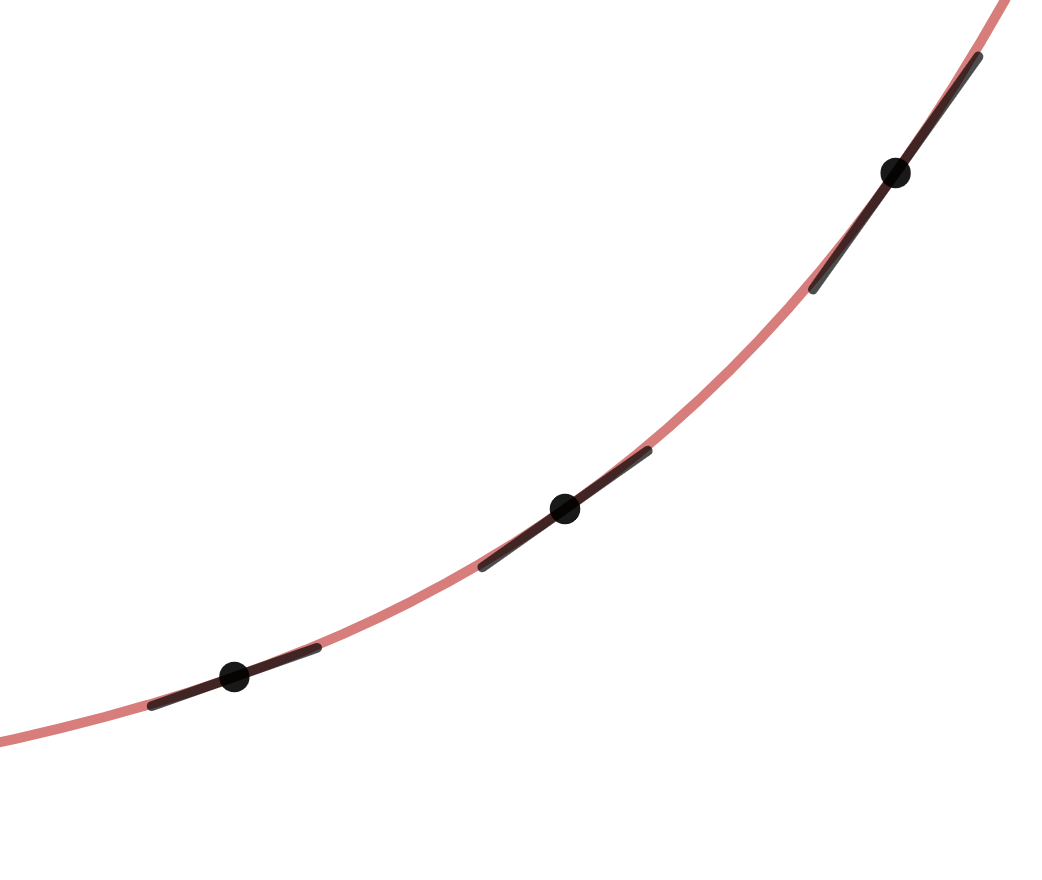
\includegraphics[width=1.5in]{./AppDerivativesGraphics/IncCU.png} 

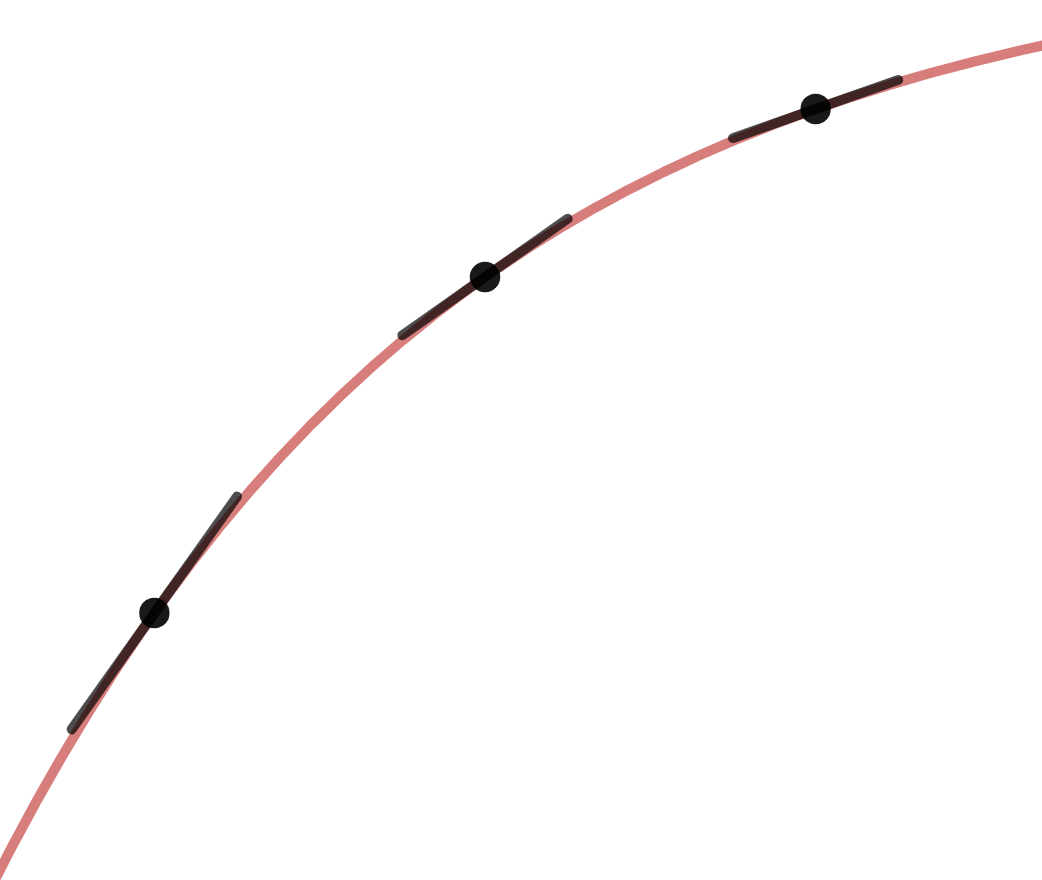
\includegraphics[width=1.5in]{./AppDerivativesGraphics/IncCD.png} 

\end{multicols}

\end{center}

\item  $f'(x) < 0$  for all $x$ in $I$:


\begin{center}

\begin{multicols}{2}

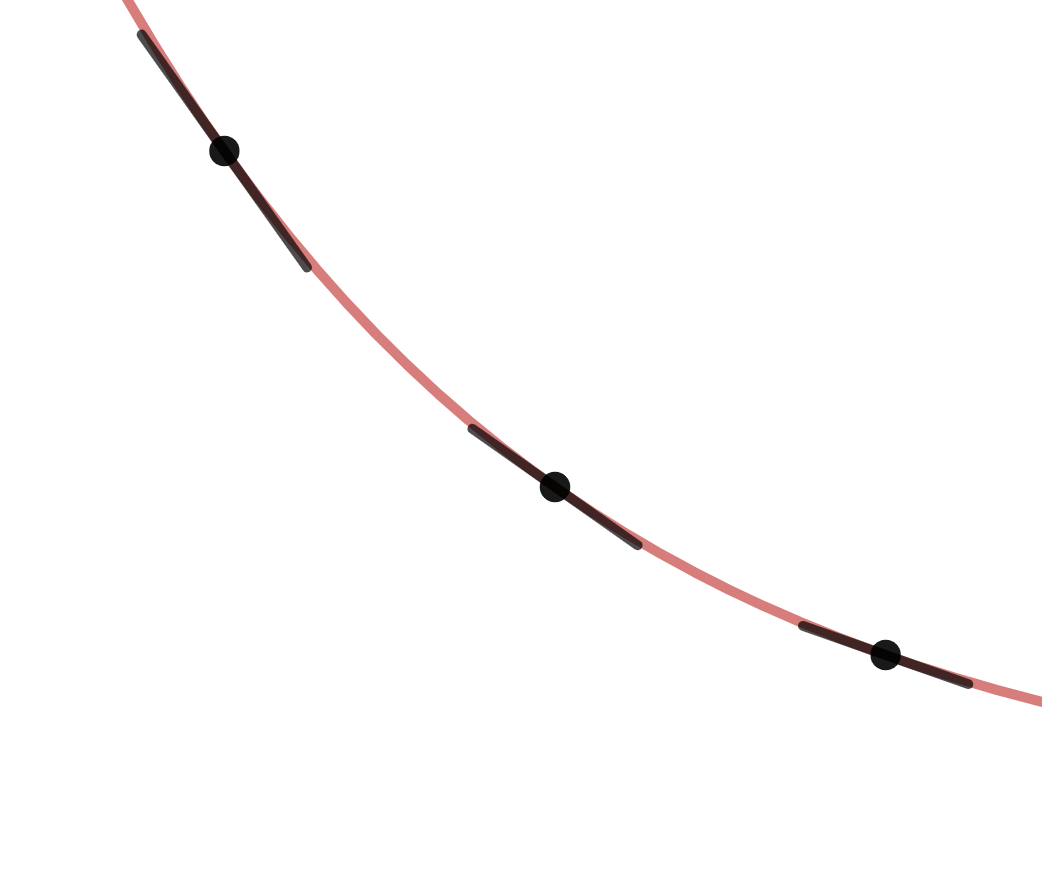
\includegraphics[width=1.5in]{./AppDerivativesGraphics/DecCU.png} 

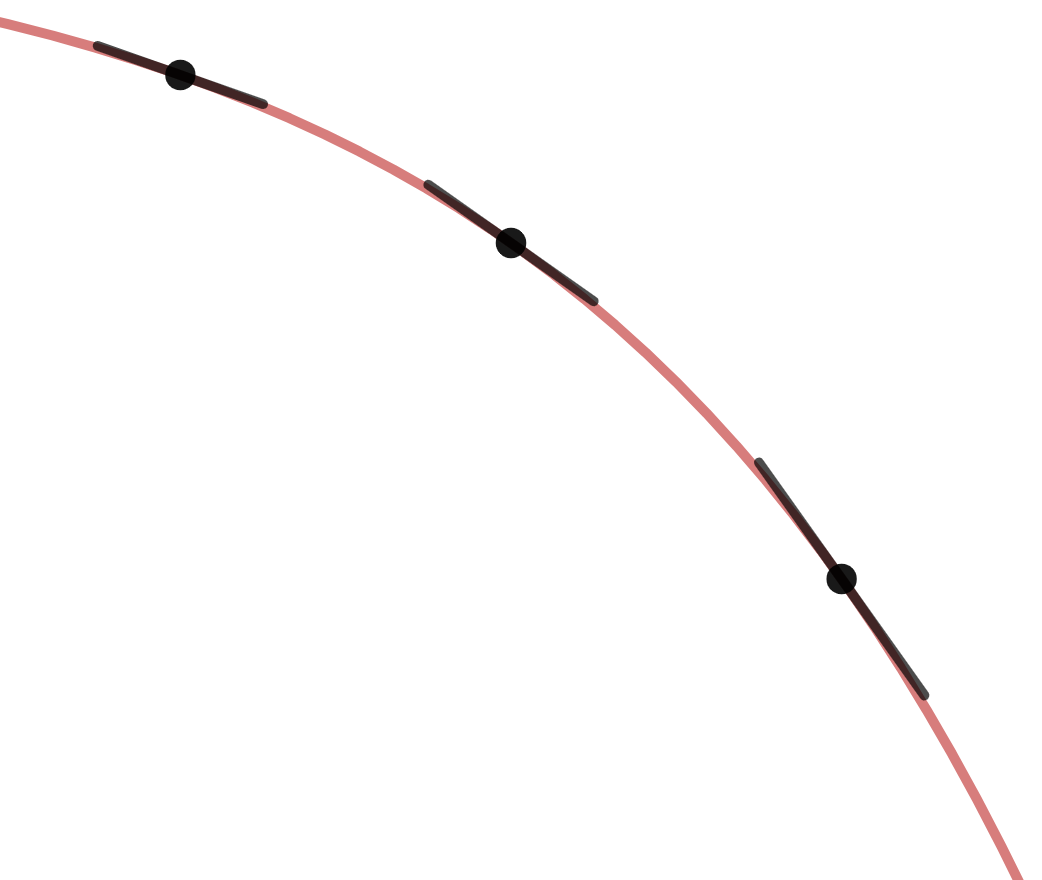
\includegraphics[width=1.5in]{./AppDerivativesGraphics/DecCD.png} 

\end{multicols}

\end{center}


\item $f'(x) = 0$  for all $x$ in $I$:

\begin{center}

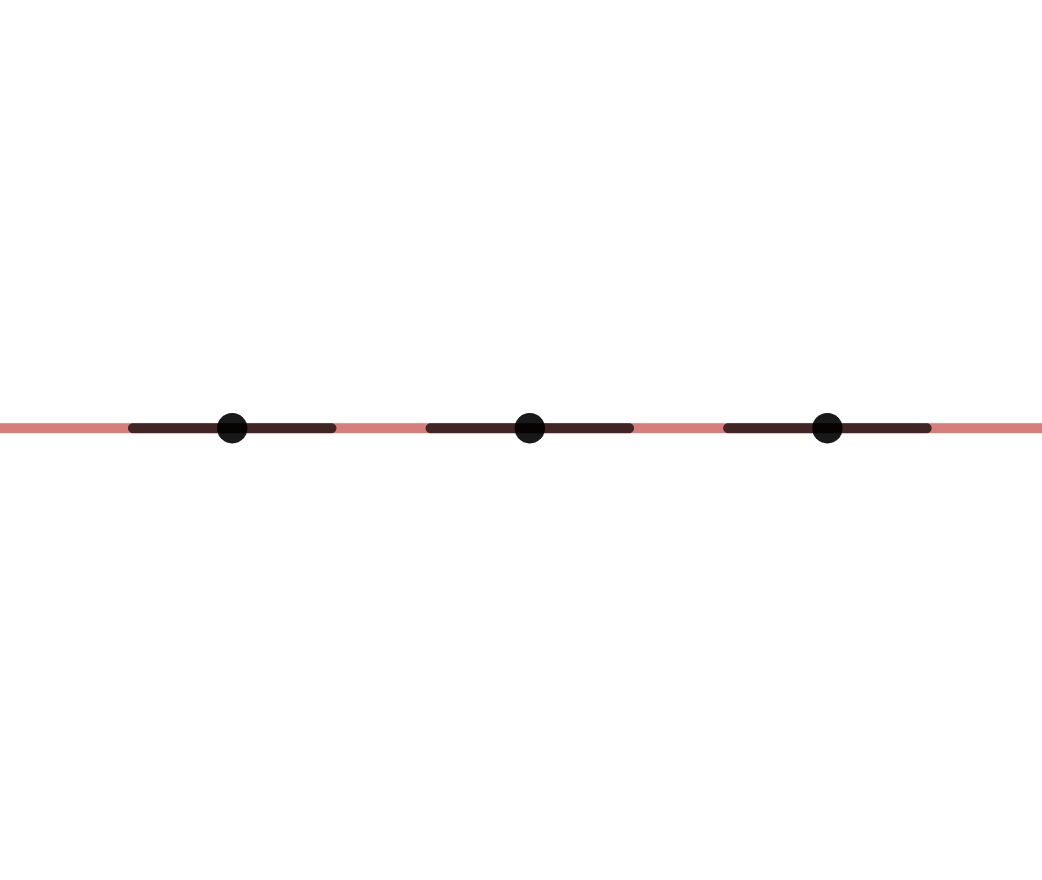
\includegraphics[width=1.5in]{./AppDerivativesGraphics/Constant.png} 

\end{center}

\end{itemize}

We can use Theorem \ref{firstderivatveandgraphs} to help us determine the (open) intervals over which a function $f$ is increasing, decreasing, and constant by making a sign diagram for the derivative $f'$. 

\medskip

In order to avoid us having to go through the (somewhat lengthy) process of finding $f'(x)$ using Definition \ref{derivativefcndefn}, we'll just use some properties of derivatives from Calculus behind the scenes and present you with both a function and its derivative.  It's time for an example.

\medskip

\begin{example}\label{polyincdec}  Let  $f(x) = x^3 - 3x^2 - 9x+5$.  Use the fact that $f'(x) = 3x^2-6x-9$  to find the open intervals over which $f$ is increasing, decreasing, and constant.  Check your answer graphically.

\medskip


{\bf Solution.}   To make use of  Theorem \ref{firstderivatveandgraphs}, we make a sign diagram for $f'(x)$.  Since $f'$ is a polynomial, $f'$ is continuous so the per the Intermediate Value Theorem, Theorem \ref{IVT}, $f'$ will only change sign on either side of zeros.  Hence, our first step is to solve  $f'(x) = 0$.  


\medskip

We are given  $f'(x) = 3x^2-6x-9$.   Solving $f'(x) =  3x^2-6x-9 = 0$  gives  $3(x^2-2x-3) = 0$ or   $3(x-3)(x+1) = 0$.  We get two solutions:  $x = -1$ and $x = 3$ which divides the $x$-axis into three regions:  $x< -1$, $-1<x<3$ and $x>3$. 

\medskip

Next we select a test value in each of these three regions to determine the sign of $f'(x)$.  For the interval $x<-1$, we select $x = -3$:   $f'(-3) = 3(-3)^2-6(-3)-9 = (+)$.  For $-1<x<3$, we select $x = 0$:  $f'(0) =  3(0)^2-6(0)-9 = (-)$. Finally, for $x>3$, we select $x = 4$:  $f'(4) = 3(4)^2-6(4)-9  = (+)$.

\medskip

Below on the left is a sign diagram for $f'(x)$ and on the right is what this means for the graph of $y=f(x)$:

\begin{center}

\begin{multicols}{2}

\begin{mfpic}[15]{-6}{6}{-2}{2}
\arrow \reverse \arrow \polyline{(-5,0),(5,0)}
\xmarks{-2,2}
\arrow \polyline{(-3.5,-1.5),(-3.5,-0.5)}
\arrow \polyline{(0,-1.5),(0,-0.5)}
\arrow \polyline{(3.5,-1.5),(3.5,-0.5)}
\tlpointsep{4pt}
\axislabels {x}{{$-1 \hspace{7pt}$} -2, {$3$} 2}
\tlabel[cc](-3.5,1){$(+)$}
\tlabel[cc](-2,1){$0$}
\tlabel[cc](0,1){$(-)$}
\tlabel[cc](2,1){$0$}
\tlabel[cc](3.5,1){$(+)$}
\tlabel[cc](-3.75,-2.25){$-3$}
\tlabel[cc](0,-2.25){$0$}
\tlabel[cc](3.6,-2.25){$4$}
\tlabel[cc](6,1){$f'(x)$}
\tlabel[cc](6,-1){$x$}
%\tlabel[cc](6,0){$\infty$}
%\tlabel[cc](-6,0){$-\infty$}
\end{mfpic}

\begin{mfpic}[15]{-6}{6}{-2}{2}
\arrow \reverse \arrow \polyline{(-5,0),(5,0)}
\xmarks{-2,2}
%\arrow \polyline{(-3.5,-1.5),(-3.5,-0.5)}
%\arrow \polyline{(0,-1.5),(0,-0.5)}
%\arrow \polyline{(3.5,-1.5),(3.5,-0.5)}
\tlpointsep{4pt}
\axislabels {x}{{$-1\hspace{7pt}$} -2, {$3$} 2}
\tlabel[cc](-3.5,1){$\nearrow$}
\tlabel[cc](-2,1){$\rightarrow$}
\tlabel[cc](0,1){$\searrow$}
\tlabel[cc](2,1){$\rightarrow$}
\tlabel[cc](3.5,1){$\nearrow$}
%\tlabel[cc](-3.75,-2.25){$-3$}
%\tlabel[cc](0,-2.25){$0$}
%\tlabel[cc](3.6,-2.25){$4$}
\tlabel[cc](6,1){$f(x)$}
\tlabel[cc](6,-1){$x$}
%\tlabel[cc](6,0){$\infty$}
%\tlabel[cc](-6,0){$-\infty$}
\end{mfpic}


\end{multicols}
\end{center}

We find $f$ is increasing on $(-\infty, -1)$ and again on $(3, \infty)$ while  $f$ is decreasing on $(-1,3)$.  At the points $x = -1$ and $x=3$, we have $f'(x) = 0$ so the graph of $f$ is locally flat there.  

\medskip

Since $f$ changes from increasing just to the left of $x=-1$ to decreasing just to the right of $x=-1$, it stands to reason that $f$ has a local maximum at $x=-1$.  This is indeed the case and we find that the local maximum value is  $f(-1) = (-1)^3 - 3(-1)^2 - 9(-1)+5 = 10$.

\medskip

Similarly, since $f$ changes from decreasing just to the left of $x=3$ to increasing just to the right of $x=3$, $f$ has a local minimum at $x=3$.  The local minimum value is $f(3) = (3)^3 - 3(3)^2 - 9(3)+5 = -22$.

\medskip


A quick check using desmos confirms our results.

\medskip

\centerline{ 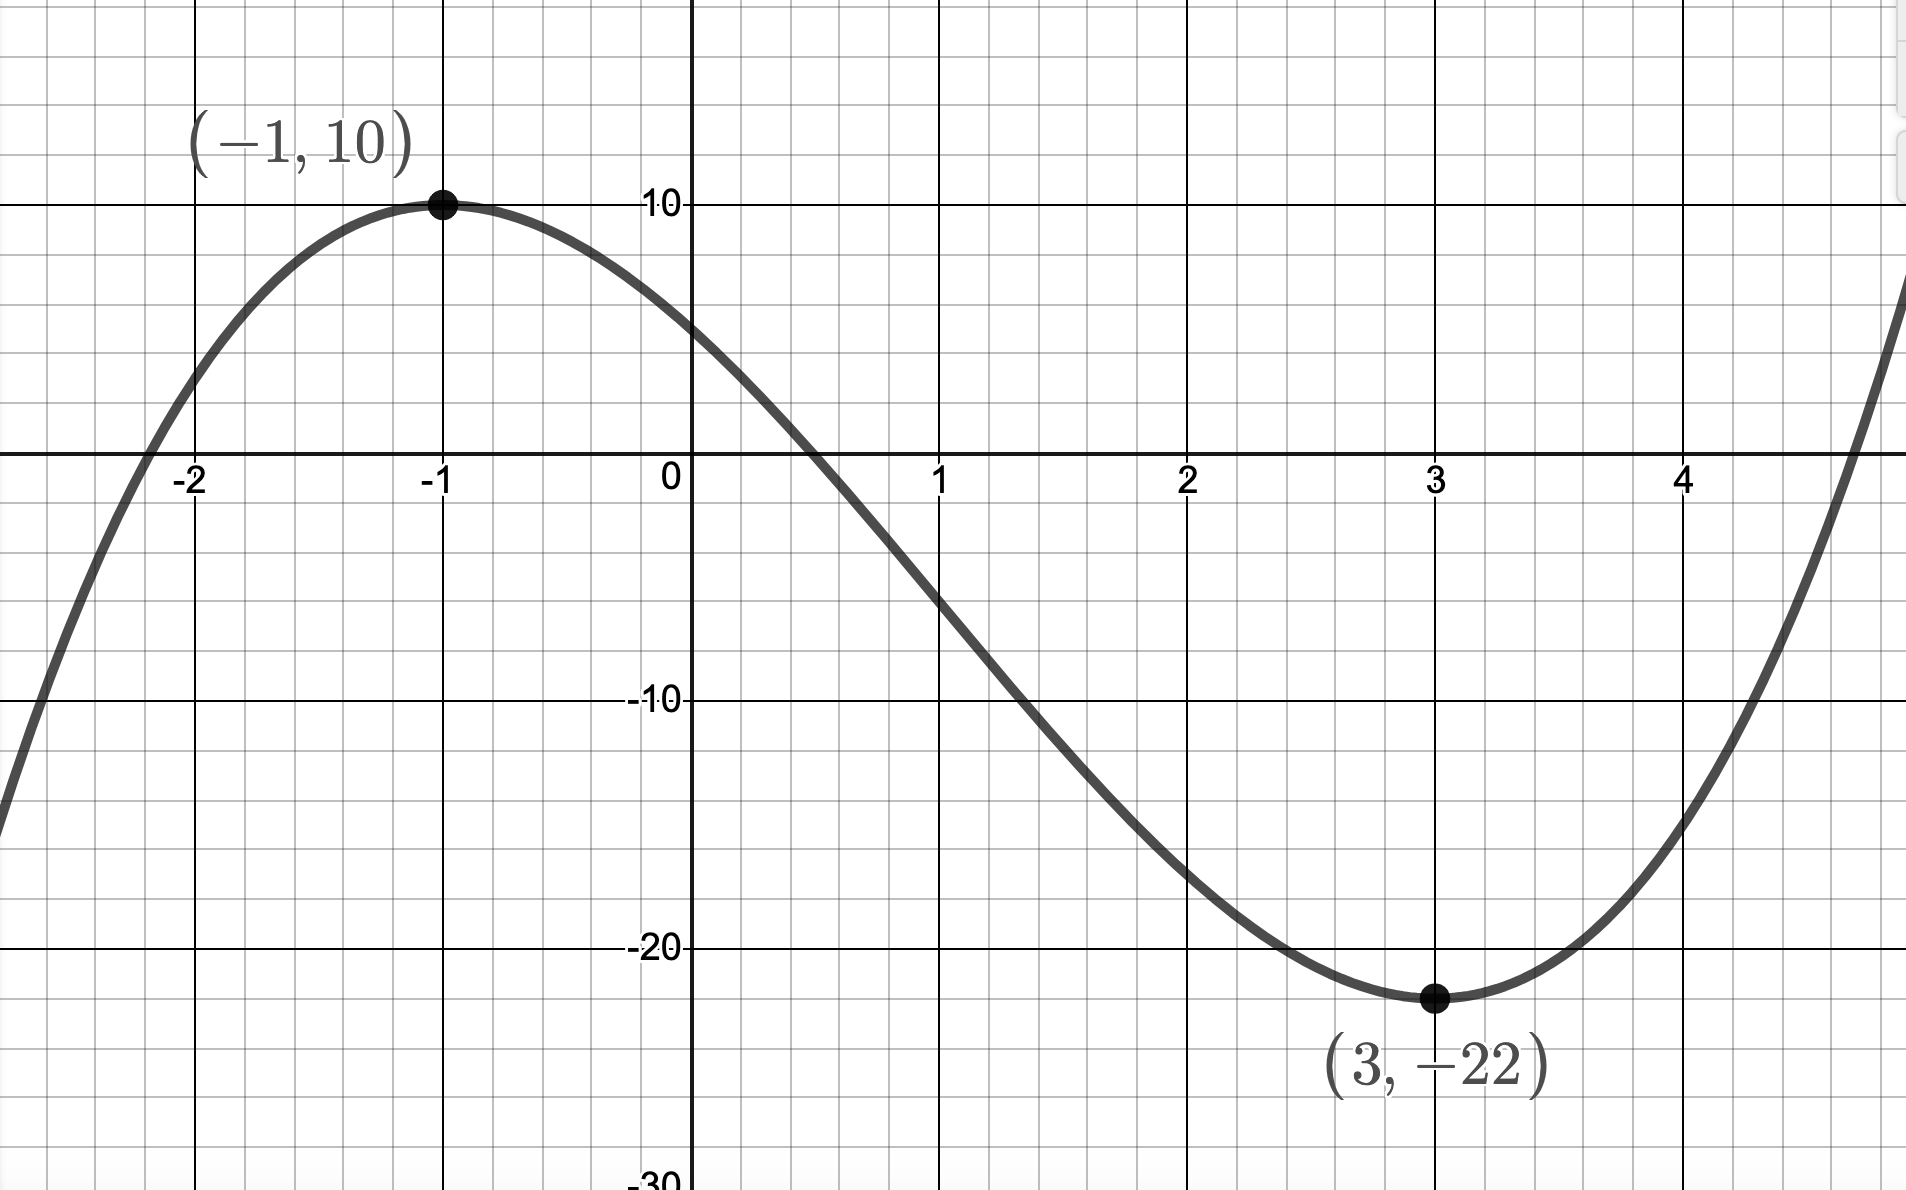
\includegraphics[width=4in]{./AppDerivativesGraphics/IncDecPoly.png}}

\hfill \qed

\end{example}

We generalize our observations about local extrema in the following result.

\medskip

%% \colorbox{ResultColor}{\bbm

\begin{theorem}  \label{firstderivatvetest}   \textbf{The (First)\footnote{Why `First'?  Stay tuned \ldots} Derivative Test for Local Extema:}  Let $f$ be continuous on an open interval $I$ containing a critical number $c$.\footnote{Recall this means $f'(c) = 0$ or $f'(c)$ does not exist.}  If $f$ is differentiable on $I$, except possibly at $c$, then  

\medskip

\begin{itemize}

\item If $f'(x)$ changes from $(+)$ for $x<c$ to $(-)$ for $x>c$, $f$ has a local maximum at $x=c$.

\item If $f'(x)$ changes from $(-)$ for $x<c$ to $(+)$ for $x>c$, $f$ has a local minimum at $x=c$.

\item If $f'(x)$ doesn't change sign going from $x<c$ to $x>c$, $f$ does not have a local extremum at $x=c$.

\end{itemize}

\end{theorem}
%% \ebm}

\medskip

\begin{example} \label{powerfcnincdec} Let $f(x) = x^{4/3} - 4x^{1/3}$. Use the fact that $f'(x) = \frac{4}{3} x^{1/3} - \frac{4}{3} x^{-2/3}$ to help you find:

\begin{enumerate}

\item the open intervals over which $f$ is increasing, decreasing, and constant.

\item the local extrema.

\end{enumerate}

{\bf Solution.}    \begin{enumerate}  \item In order to make a sign diagram for $f'(x)$, we rewrite $f'(x)$ as a single fraction:  \[f'(x) = \dfrac{4}{3} x^{1/3} - \dfrac{4}{3} x^{-2/3} =  \dfrac{4x^{1/3}}{3}  - \dfrac{4}{3x^{2/3}}  = \dfrac{4x^{1/3}}{3} \cdot \dfrac{x^{2/3}}{x^{2/3}} - \dfrac{4}{3x^{2/3}} = \dfrac{4x}{3x^{2/3}} - \dfrac{4}{3x^{2/3}}   = \dfrac{4x-4}{3x^{2/3}}.\]

\medskip

Unlike the derivative in Example \ref{polyincdec}, $f'(x) =  \frac{4x-4}{3x^{2/3}}$ is undefined when $3x^{2/3} = 0$, that is, when $x = 0$, so we need to record this on our sign diagram with the customary `\textinterrobang.'  

\medskip

Next, we solve  $f'(x) =  \frac{4x-4}{3x^{2/3}} = 0$ to get $4x-4 = 0$ or $x = 1$. The usual machinations produces the  sign diagram for $f'(x)$ below on the left.  We interpret what this means for $f$ below on the right.

\medskip

\begin{center}

\begin{multicols}{2}

\begin{mfpic}[15]{-6}{6}{-2}{2}
\arrow \reverse \arrow \polyline{(-5,0),(5,0)}
\xmarks{-2,2}
\arrow \polyline{(-3.5,-1.5),(-3.5,-0.5)}
\arrow \polyline{(0,-1.5),(0,-0.5)}
\arrow \polyline{(3.5,-1.5),(3.5,-0.5)}
\tlpointsep{4pt}
\axislabels {x}{{$0$} -2, {$1$} 2}
\tlabel[cc](-3.5,1){$(-)$}
\tlabel[cc](-2,1){\textinterrobang}
\tlabel[cc](0,1){$(-)$}
\tlabel[cc](2,1){$0$}
\tlabel[cc](3.5,1){$(+)$}
\tlabel[cc](-3.75,-2.25){$-1$}
\tlabel[cc](0,-2.25){$\frac{1}{2}$}
\tlabel[cc](3.6,-2.25){$2$}
\tlabel[cc](6,1){$f'(x)$}
\tlabel[cc](6,-1){$x$}
%\tlabel[cc](6,0){$\infty$}
%\tlabel[cc](-6,0){$-\infty$}
\end{mfpic}

\begin{mfpic}[15]{-6}{6}{-2}{2}
\arrow \reverse \arrow \polyline{(-5,0),(5,0)}
\xmarks{-2,2}
%\arrow \polyline{(-3.5,-1.5),(-3.5,-0.5)}
%\arrow \polyline{(0,-1.5),(0,-0.5)}
%\arrow \polyline{(3.5,-1.5),(3.5,-0.5)}
\tlpointsep{4pt}
\axislabels {x}{{$0$} -2, {$1$} 2}
\tlabel[cc](-3.5,1){$\searrow$}
\tlabel[cc](-2,1){\textinterrobang}
\tlabel[cc](0,1){$\searrow$}
\tlabel[cc](2,1){$\rightarrow$}
\tlabel[cc](3.5,1){$\nearrow$}
%\tlabel[cc](-3.75,-2.25){$-3$}
%\tlabel[cc](0,-2.25){$0$}
%\tlabel[cc](3.6,-2.25){$4$}
\tlabel[cc](6,1){$f(x)$}
\tlabel[cc](6,-1){$x$}
%\tlabel[cc](6,0){$\infty$}
%\tlabel[cc](-6,0){$-\infty$}
\end{mfpic}


\end{multicols}
\end{center}

We get $f$ is decreasing for $x<0$ as well as from $0 < x < 1$.  Since $0$ is in the domain of $f$, we splice the two intervals together so $f$ is decreasing from $(-\infty, 1)$.  We see $f$ is increasing from $(1, \infty)$.

\medskip

\item   We note that $f$ satisfies the conditions of Theorem \ref{firstderivatvetest} since $f$ is continuous everywhere and $f'$ exists for all $x \neq 0$.  Since $f$ changes from decreasing just to the left of $x=1$ to increasing just to the right of $x=1$,  the graph of $f$ has a local minimum at $x=1$.  The local minimum value is $f(1) = (1)^{4/3} - 4(1)^{1/3} = -3$. 

\medskip

What is happening at $x = 0$?  Since $f'(x)$ doesn't change sign on either side of $0$,  the graph of $f$ doesn't have a local extremum there.  The sign diagram indicates  $f$ is decreasing through that point.  A quick check using desmos reveals `unsual steepness' at $x = 0$, a phenomenon which is called a \index{vertical tangent}\index{tangent ! vertical}\textbf{vertical tangent}. This means the function locally resembles a vertical line.\footnote{See Example \ref{rootradicalfcnex} for another such example and discussion.}

\medskip

\centerline{ 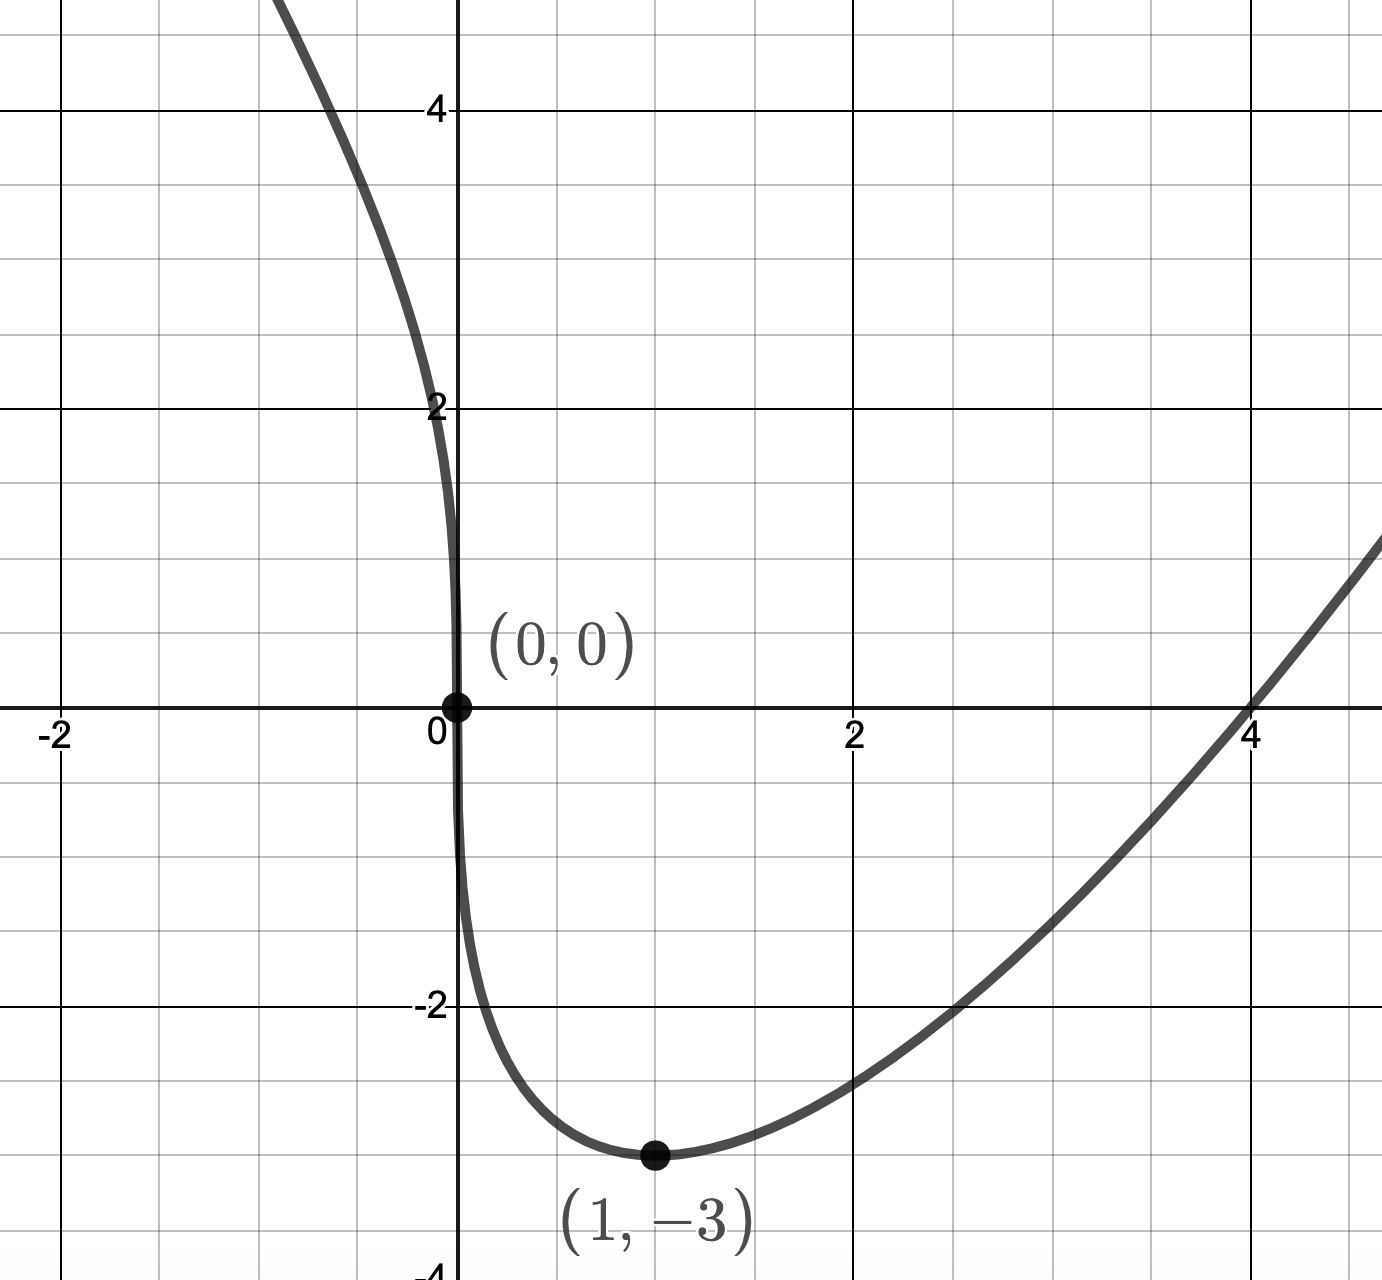
\includegraphics[width=3in]{./AppDerivativesGraphics/IncDecRoot.png}}

\end{enumerate}

\hfill \qed

\end{example}


\subsection{Concavity and the Second Derivative}
\label{concavity}

In section Section \ref{PowerFunctions}, we introduced the notion of \index{concavity}\textbf{concavity}.  In that section, we described curves as  being  \index{concave up}\index{concavity ! concave up}\textbf{concave up} over an interval if it resembles a  portion of a `$\smile$' shape and   \index{concave down}\index{concavity ! concave down}\textbf{concave down} over an interval if resembles part of a `$\frown$' shape. Now that we've had some exposure to Calculus, we can more precisely define these notions.

\medskip


%% \colorbox{ResultColor}{\bbm

\begin{definition}  \label{concavitydefn} Let $f$ be a differentiable function on an open interval  $I$.  Then $f$ is said to be:

\begin{itemize}

\item  \textbf{concave up} on $I$ if the tangent lines lie \textbf{below} the graph on $I$.

\item  \textbf{concave down} on $I$ if the tangent lines lie \textbf{above} the graph on $I$.

\smallskip

\end{itemize}

\end{definition}

%% \ebm}

\pagebreak

If we take the time to study a generic concave up curve, the `$\smile$' shape can be divided into a decreasing and increasing arc:

\begin{center}

\begin{multicols}{2}

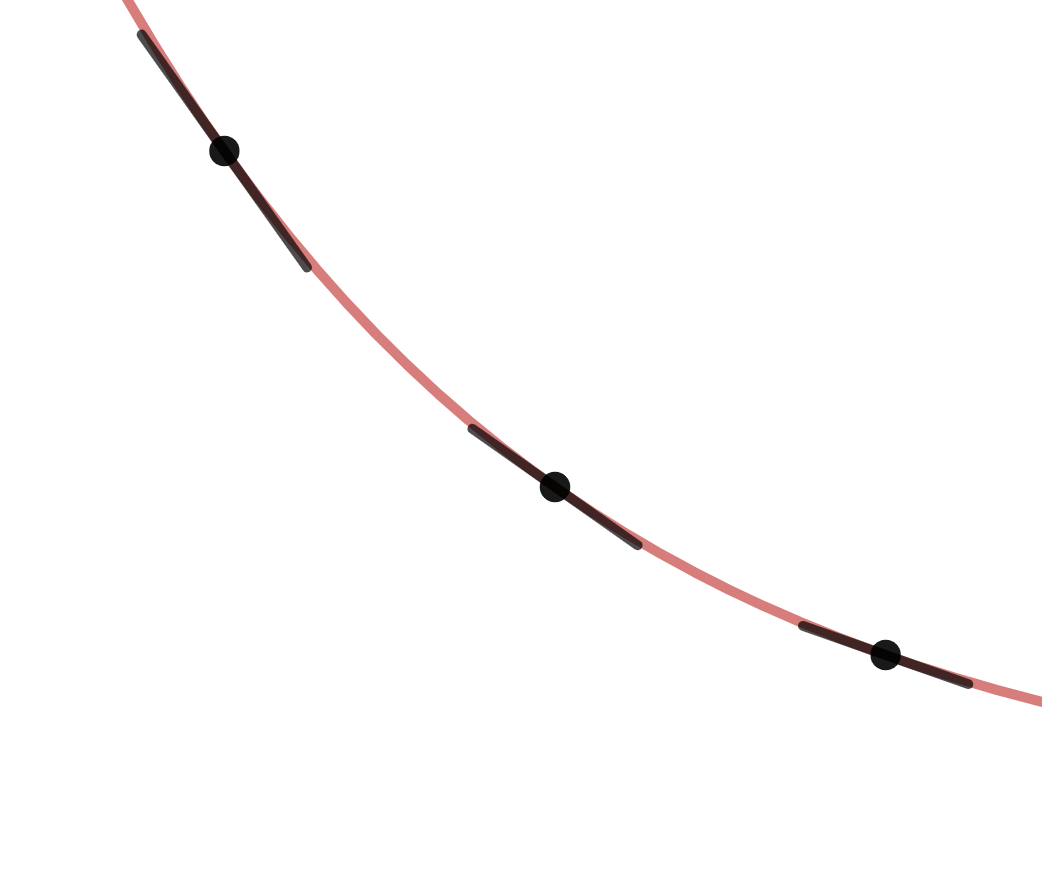
\includegraphics[width=1.5in]{./AppDerivativesGraphics/DecCU.png} 

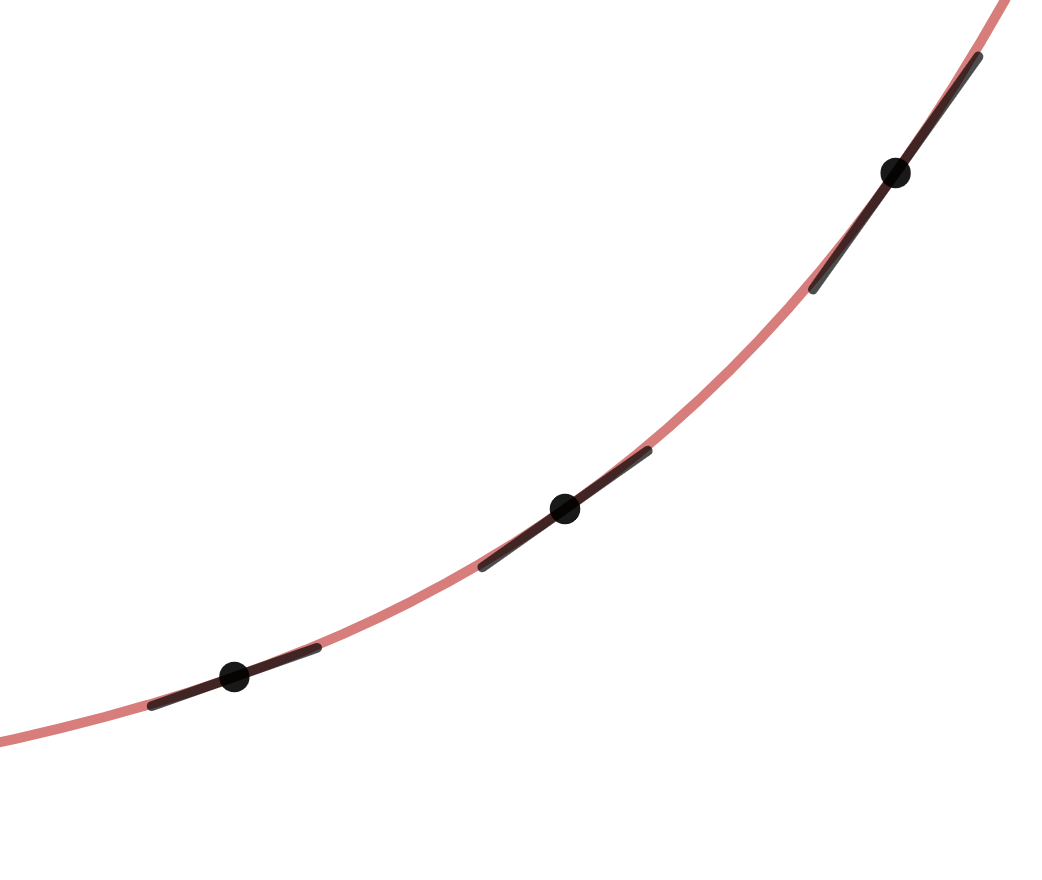
\includegraphics[width=1.5in]{./AppDerivativesGraphics/IncCU.png} 


\end{multicols}

\end{center}

\begin{center}

\begin{multicols}{2}

slopes are increasing towards $0$

slopes are increasing away from $0$

\end{multicols}

\end{center}

In both of these cases, the \textbf{slopes} of the tangent line are \textbf{increasing}.  

\medskip

Likewise, we can dissect a generic `$\frown$' shape curve into an increasing and decreasing arc:

\begin{center}

\begin{multicols}{2}

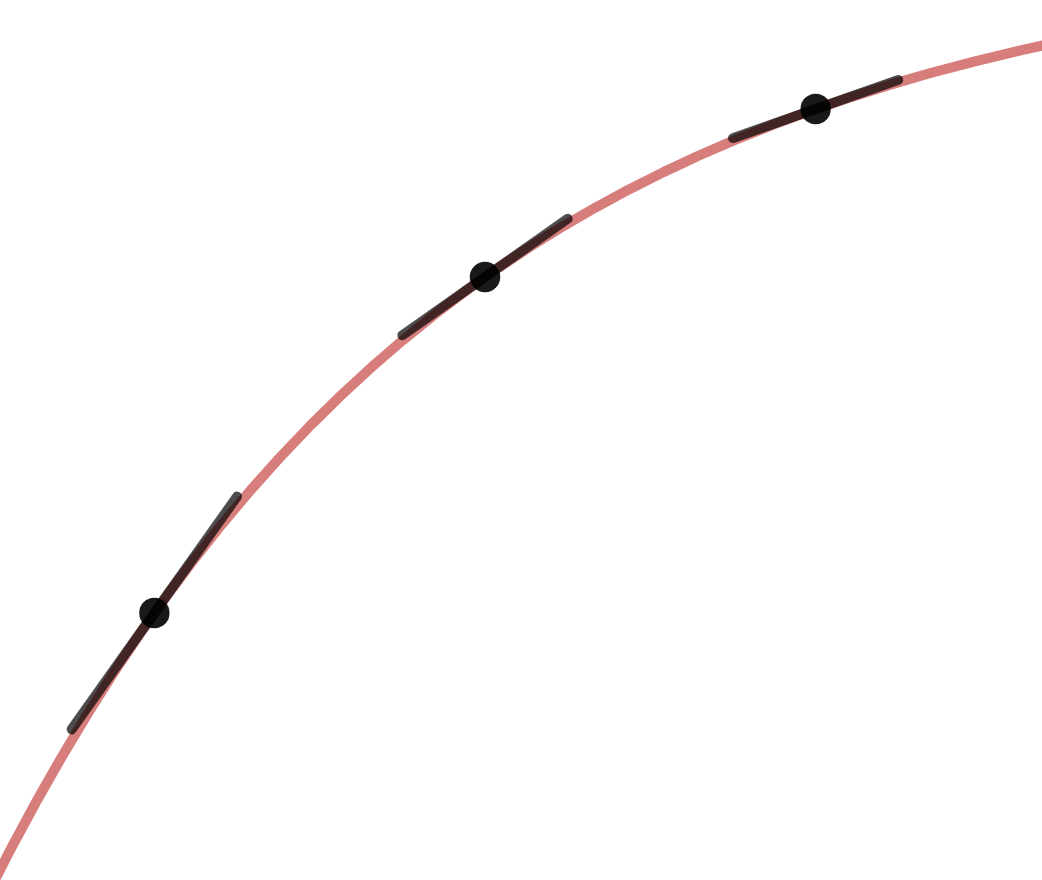
\includegraphics[width=1.5in]{./AppDerivativesGraphics/IncCD.png} 

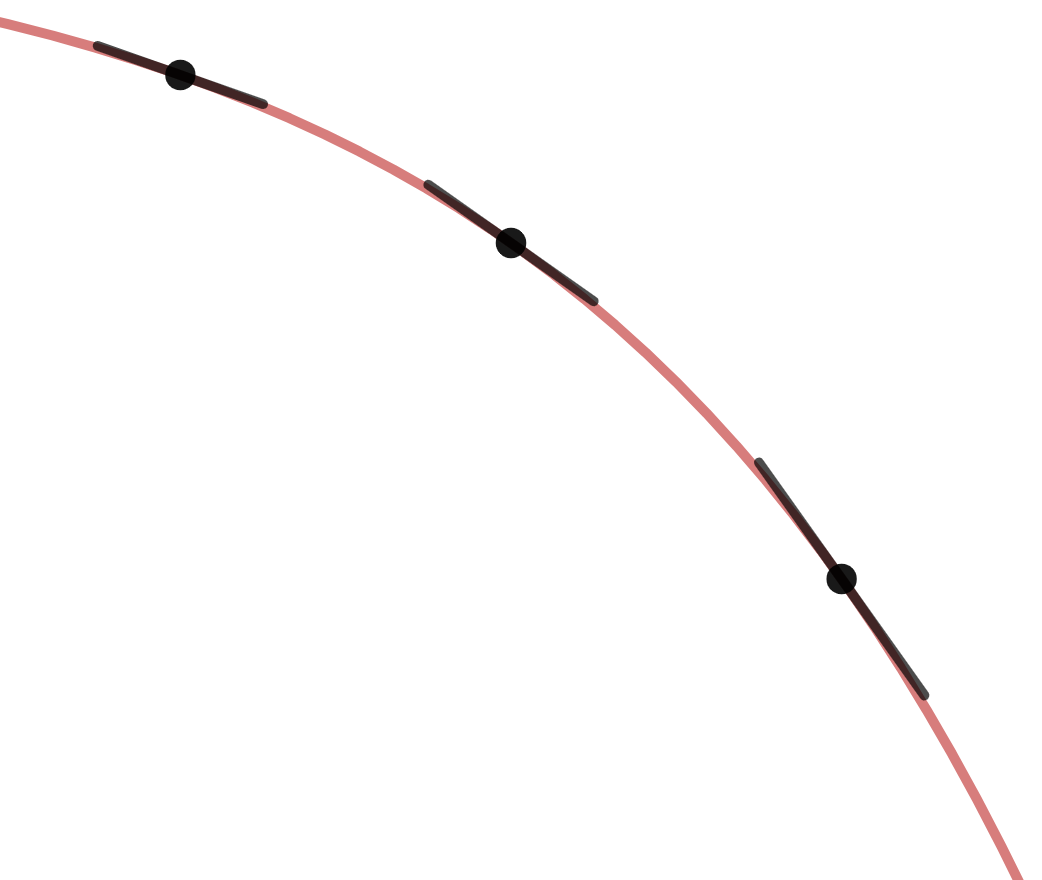
\includegraphics[width=1.5in]{./AppDerivativesGraphics/DecCD.png} 

\end{multicols}

\end{center}

\begin{center}

\begin{multicols}{2}

slopes are decreasing towards $0$

slopes are decreasing away from $0$

\end{multicols}

\end{center}

Here, the \textbf{slopes} of the tangent line are \textbf{decreasing}.  

\medskip

We know from Theorem \ref{firstderivatveandgraphs} that the derivative of a function can tell us where that function is increasing and decreasing.  Since the function which gives us the slopes of tangent lines is the derivative, $f'(x)$, we could use the derivative of $f'(x)$ to determine where the slopes of the tangent lines were increasing and decreasing.  This leads us to define the \index{second derivative}\index{derivative ! second}\textbf{second derivative}, $f''(x)$  as the derivative of $f'(x)$.

\medskip

We present the following theorem without proof, but hopefully sufficiently motivated. 

\medskip

%% \colorbox{ResultColor}{\bbm

\begin{theorem}  \label{secondderivatveandgraphs}   Suppose $f$ is twice differentiable on an open interval $I$:

\begin{itemize}

\item If $f''(x) > 0$ for all $x$ in $I$, then \textbf{slopes} are \textbf{increasing} and  $f$ is \textbf{concave up} on $I$.  

\item If $f''(x) < 0$ for all $x$ in $I$, then \textbf{slopes} are \textbf{decreasing} and  $f$ is \textbf{concave down} on $I$. 

\end{itemize}

\end{theorem}

%% \ebm}


\pagebreak

\begin{example}\label{polyconcavity} Let $f(x) = x^3 - 3x^2 - 9x+5$.  Use the fact that $f''(x) = 6x-6$ to find the intervals over which the graph of $f$ is concave up and concave down.

\medskip

{\bf Solution.}  To analyze the concavity of the graph of $f$, we need to make a sign diagram for $f''(x)$.  

\medskip

Solving $f''(x) = 6x-6 = 0$ gives $x=1$. We find $f''(0) =  6(0)-6 = (-)$ and $f''(2) = 6(2) - 6=  (+)$.  

\medskip

We have our sign diagram below on the left and our interpretation below on the right.

\begin{center}

\begin{multicols}{2}

\begin{mfpic}[15]{-6}{6}{-2}{2}
\arrow \reverse \arrow \polyline{(-5,0),(5,0)}
\xmarks{0}
\arrow \polyline{(-2,-1.5),(-2,-0.5)}
\arrow \polyline{(2,-1.5),(2,-0.5)}
\tlpointsep{4pt}
\axislabels {x}{{$1$} 0}
\tlabel[cc](-2,1){$(-)$}
\tlabel[cc](0,1){$0$}
\tlabel[cc](2,1){$(+)$}
\tlabel[cc](-2,-2.25){$0$}
\tlabel[cc](2,-2.25){$2$}
\tlabel[cc](6,1){$f''(x)$}
\tlabel[cc](6,-1){$x$}
%\tlabel[cc](6,0){$\infty$}
%\tlabel[cc](-6,0){$-\infty$}
\end{mfpic}

\begin{mfpic}[15]{-6}{6}{-2}{2}
\arrow \reverse \arrow \polyline{(-5,0),(5,0)}
\xmarks{0}
%\arrow \polyline{(-2,-1.5),(-2,-0.5)}
%\arrow \polyline{(2,-1.5),(2,-0.5)}
\tlpointsep{4pt}
\axislabels {x}{{$1$} 0}
\tlabel[cc](-2,1){\huge $\frown$}
%\tlabel[cc](0,1){$0$}
\tlabel[cc](2,1){\huge $\smile$}
%\tlabel[cc](-2,-2.25){$0$}
%\tlabel[cc](2,-2.25){$2$}
\tlabel[cc](6,1){$f(x)$}
\tlabel[cc](6,-1){$x$}
%\tlabel[cc](6,0){$\infty$}
%\tlabel[cc](-6,0){$-\infty$}
\end{mfpic}


\end{multicols}
\end{center}

We find $f$ is concave down on $(-\infty, 1)$ and concave up on $(1, \infty)$.  

\medskip

At $x=1$, the concavity changes.  We find $f(1) = (1)^3 - 3(1)^2 - 9(1)+5 = -6$ and we call the point $(1, -6)$ an \textbf{inflection point}.  In this case since the concavity changes from concave down to concave up, the point $(1,-6)$ is the point on the graph of $y=f(x)$ were the slopes stop decreasing and start to increase.

\medskip

A quick check using desmos confirms our results.

\medskip

\centerline{ 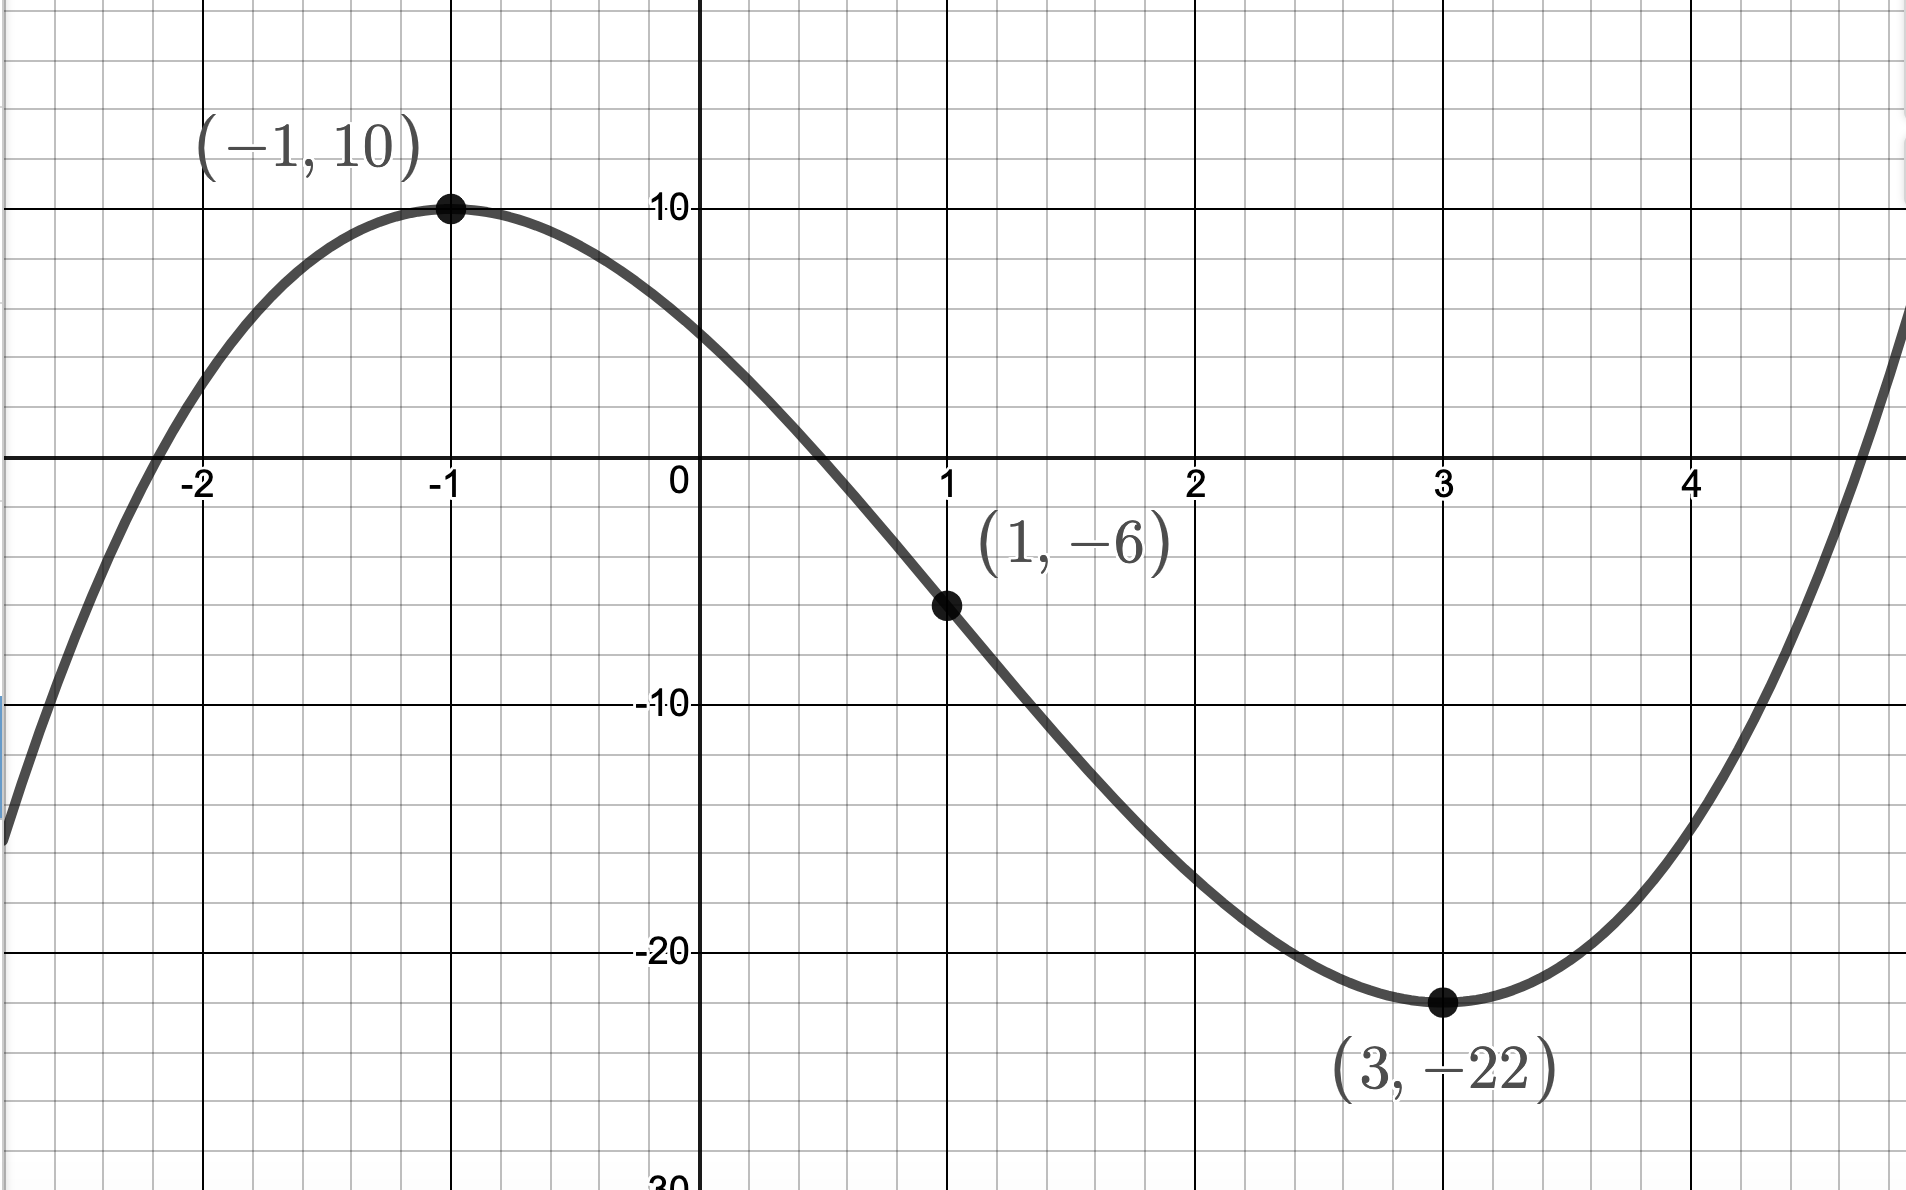
\includegraphics[width=4in]{./AppDerivativesGraphics/ConcavityPoly.png}}

\hfill \qed

\end{example}

\medskip

Note that we can use concavity to help us distinguish local extrema.  

\medskip

For the function above, both $f'(-1) = 0$ and $f'(3) = 0$.  Note that $f''(-1) < 0$ which means $f$ is concave down there. This forces $f$ to have a local maximum at $(-1,6)$.  Likewise, $f''(3) > 0$ which means $f$ is concave up there.  This forces $f$ to have a local minimum at $(3,-22)$.  We generalize this observation below.

\medskip



%% \colorbox{ResultColor}{\bbm

\begin{theorem}  \label{secondderivatvetest}   \textbf{The Second\footnote{Now you know why we titled Theorem \ref{firstderivatvetest} the `First' Derivative Test for Local Extrema.} Derivative Test for Local Extrema:}  Suppose $f$ is differentiable on an open interval $I$ containing $c$ and $f'(c) = 0$:

\begin{itemize}

\item If $f''(c) > 0$ then $f$ has a local minimum at $x=c$.

\item If $f''(c) < 0$ then $f$ has a local maximum at $x=c$.

\item If $f''(c) = 0$ then the test is inconclusive.  $f$ may or may not have a local extremum at $x=c$.  

(In this case, we would appeal to the first derivative test.)

\end{itemize}
\end{theorem}

%% \ebm}



\medskip

\begin{example} \label{powerfcnconcavity}  Let $f(x) = x^{4/3} - 4x^{1/3}$.   Use the fact that $f''(x) =  \frac{4}{9} x^{-2/3} + \frac{8}{9} x^{-5/3}$ to help you find:

\begin{enumerate}

\item  the open intervals over which the graph of $f$ is concave up and concave down.

\item  the inflection points in the graph.

\end{enumerate}

\medskip

{\bf Solution.}

\begin{enumerate} \item  As in Example \ref{powerfcnincdec}, our first step is to  rewrite  $f''(x) =  \frac{4}{9} x^{-2/3} + \frac{8}{9} x^{-5/3}$  as a single fraction:


\[ f''(x) = \dfrac{4}{9} x^{-2/3} + \dfrac{8}{9} x^{-5/3} = \dfrac{4}{9x^{2/3}} + \dfrac{8}{9x^{5/3}} =  \dfrac{4}{9x^{2/3}} \cdot \dfrac{x^{3/3}}{x^{3/3}}+ \dfrac{8}{9x^{5/3}}  =  \dfrac{4x}{9x^{5/3}} + \dfrac{8}{9x^{5/3}}   =  \dfrac{4x+8}{9x^{5/3}}  \]

\medskip

We see $f''(x) =  \frac{4x+8}{9x^{5/3}} $ is undefined when $9x^{5/3}= 0$, that is, when $x = 0$.  

\medskip

Solving $f''(x) =  \frac{4x+8}{9x^{5/3}}  = 0$ gives $4x+8 = 0$ so $x = -2$. 

\newpage

Going through the usual routine, we obtain our sign diagram for $f''(x)$ is below.

\medskip

\begin{center}

\begin{multicols}{2}

\begin{mfpic}[15]{-6}{6}{-2}{2}
\arrow \reverse \arrow \polyline{(-5,0),(5,0)}
\xmarks{-2,2}
\arrow \polyline{(-3.5,-1.5),(-3.5,-0.5)}
\arrow \polyline{(0,-1.5),(0,-0.5)}
\arrow \polyline{(3.5,-1.5),(3.5,-0.5)}
\tlpointsep{4pt}
\axislabels {x}{{$-2 \hspace{7 pt}$} -2, {$0$} 2}
\tlabel[cc](-3.5,1){$(+)$}
\tlabel[cc](-2,1){$0$}
\tlabel[cc](0,1){$(-)$}
\tlabel[cc](2,1){\textinterrobang}
\tlabel[cc](3.5,1){$(+)$}
\tlabel[cc](-3.75,-2.25){$-1$}
\tlabel[cc](0,-2.25){$\frac{1}{2}$}
\tlabel[cc](3.6,-2.25){$2$}
\tlabel[cc](6,1){$f''(x)$}
\tlabel[cc](6,-1){$x$}
%\tlabel[cc](6,0){$\infty$}
%\tlabel[cc](-6,0){$-\infty$}
\end{mfpic}

\begin{mfpic}[15]{-6}{6}{-2}{2}
\arrow \reverse \arrow \polyline{(-5,0),(5,0)}
\xmarks{-2,2}
%\arrow \polyline{(-3.5,-1.5),(-3.5,-0.5)}
%\arrow \polyline{(0,-1.5),(0,-0.5)}
%\arrow \polyline{(3.5,-1.5),(3.5,-0.5)}
\tlpointsep{4pt}
\axislabels {x}{{$-2 \hspace{7 pt}$} -2, {$0$} 2}
\tlabel[cc](-3.5,1){\Huge $\smile$}
%\tlabel[cc](-2,1){?}
\tlabel[cc](0,1){\Huge $\frown$}
%\tlabel[cc](2,1){?}
\tlabel[cc](3.5,1){\Huge $\smile$}
%\tlabel[cc](-3.75,-2.25){$-3$}
%\tlabel[cc](0,-2.25){$0$}
%\tlabel[cc](3.6,-2.25){$4$}
\tlabel[cc](6,1){$f(x)$}
\tlabel[cc](6,-1){$x$}
%\tlabel[cc](6,0){$\infty$}
%\tlabel[cc](-6,0){$-\infty$}
\end{mfpic}


\end{multicols}
\end{center}

We see $f$ is concave up on $(-\infty, -2)$ and again from $(0, \infty)$.  $f$ is concave down on $(-2,0)$.

\item  Since $f$ changes concavity at both $x=-2$ and $x=0$, we have inflection point at both of these values.  

\medskip

We find:  $f(-2) = (-2)^{4/3} - 4(-2)^{1/3} = 2 (2)^{1/3} + 4 (2)^{1/3} = 6 (2)^{1/3}$. So $\left(-2, 6 (2)^{1/3} \right)$ is one inflection point.  When $x = 0$, $f(0) = (0)^{4/3} - 4(0)^{1/3}  = 0$, so $(0,0)$ is the other inflection point.  

\medskip
Checking with desmos, it's not apparent that the graph of $y=f(x)$ is concave up for $x<-2$.  We invite the reader to graph $f$ and zoom out to see that characteristic of the graph.


\medskip

\centerline{ 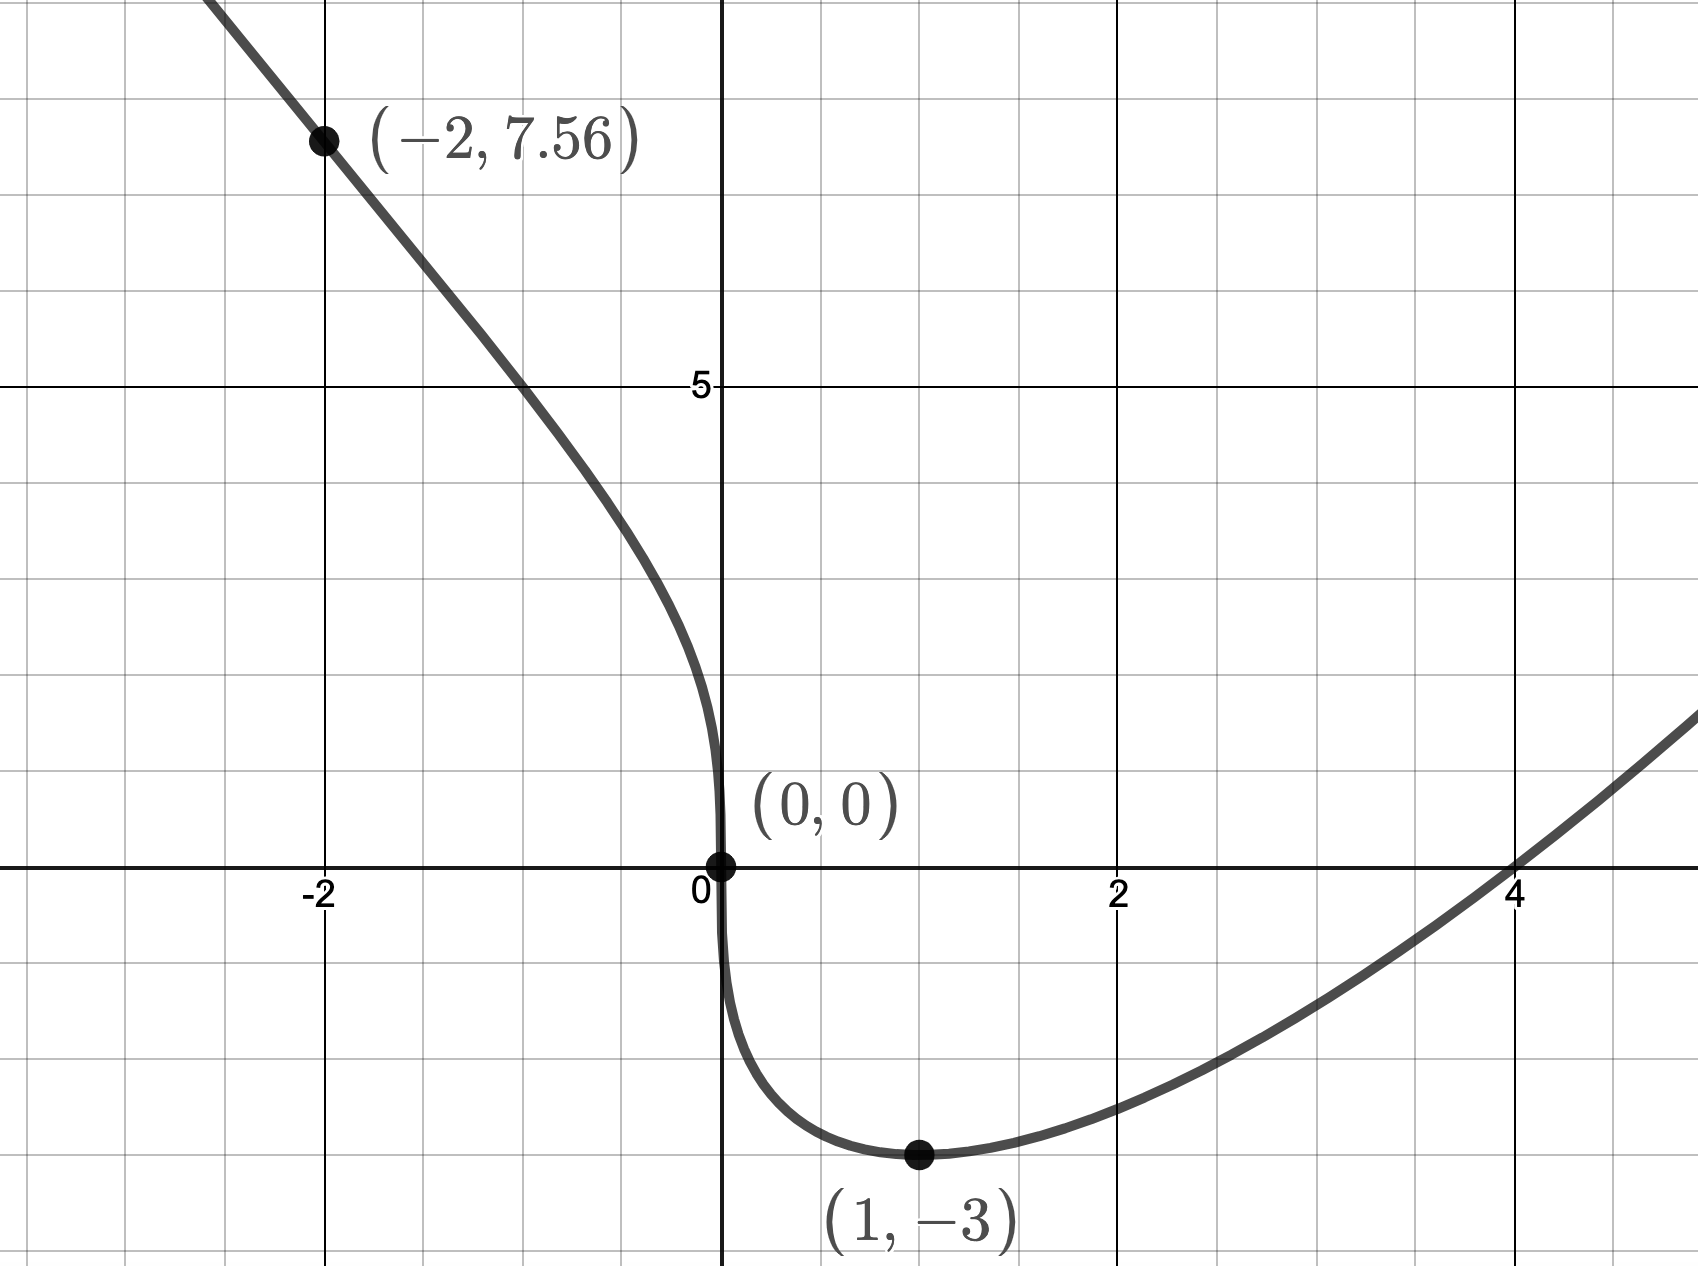
\includegraphics[width=3in]{./AppDerivativesGraphics/ConcavityRoot.png}}

\hfill \qed



\end{enumerate}

\end{example}

\medskip

Our last example offers a twist on these sorts of curve-sketching problems.

\pagebreak

\begin{example}\label{graphfromderivativegraphex} Below is the graph of the \textbf{derivative} of a function.  Assume as $x \rightarrow \pm \infty$, $f'(x) \rightarrow -\infty$.


\begin{center}

\includegraphics[width=4in]{./AppDerivativesGraphics/derivgraph.png}

The graph of $y=f'(x)$

\end{center}

\begin{enumerate}

\item  Use the graph of $y=f'(x)$ to determine the open intervals where $f$ is increasing and decreasing.  

\medskip

Find the $x$-coordinates of the local extrema.

\medskip

\item  Use the graph of $y=f'(x)$ make a sign diagram for $y=f''(x)$.

\medskip

\item  List the open intervals over which the graph of $f$ is concave up and concave down.  

\medskip

Find the $x$-coordinates of the inflection points. 

\medskip

\item  Sketch a possible graph of $y = f(x)$.

\end{enumerate}

\medskip

{\bf Solution.}

\begin{enumerate}

\item  Recall from algebra, the solutions to $f'(x) < 0$ are the $x$-values where the graph of $y = f'(x)$  is below the $x$-axis.  This happens on the intervals $(-\infty, 0)$ and $(4, \infty)$, so this means  $f$ is decreasing here.  

\medskip

Likewise,  the solutions to $f'(x) > 0$ are the $x$-values where $y=f'(x)$ is above the $x$-axis.  This happens on the interval $(0,4)$, so $f$ is increasing here.  


\medskip

Since $f$ goes from decreasing to the left of $x=0$ to increasing to the right of $x=0$, $f$ has a local minimum at $x=0$.  Since $f$ goes from increasing to the left of $x=4$ to decreasing to the right of $x=4$, $f$ has a local maximum at $x=4$.

\pagebreak


\item  Since $f''(x)$ is the derivative of $f'(x)$, we know $f''(x) > 0$ on $(-\infty, 2)$ since $f'(x)$ is increasing there.  We see $f''(2) = 0$ since $f'(x)$ is locally flat at $(2,4)$.  Lastly, we see $f''(x) < 0$ on $(2, \infty)$ since $f'(x)$ is decreasing there.  We put all this together in a sign diagram below.

\medskip

\begin{center}

\begin{multicols}{2}

\begin{mfpic}[15]{-6}{6}{-2}{2}
\arrow \reverse \arrow \polyline{(-5,0),(5,0)}
\xmarks{0}
%\arrow \polyline{(-2,-1.5),(-2,-0.5)}
%\arrow \polyline{(2,-1.5),(2,-0.5)}
\tlpointsep{4pt}
\axislabels {x}{{$2$} 0}
\tlabel[cc](-2,1){$(+)$}
\tlabel[cc](0,1){$0$}
\tlabel[cc](2,1){$(-)$}
%\tlabel[cc](-2,-2.25){$0$}
%\tlabel[cc](2,-2.25){$3$}
\tlabel[cc](6,1){$f''(x)$}
\tlabel[cc](6,-1){$x$}
%\tlabel[cc](6,0){$\infty$}
%\tlabel[cc](-6,0){$-\infty$}
\end{mfpic}

\begin{mfpic}[15]{-6}{6}{-2}{2}
\arrow \reverse \arrow \polyline{(-5,0),(5,0)}
\xmarks{0}
%\arrow \polyline{(-2,-1.5),(-2,-0.5)}
%\arrow \polyline{(2,-1.5),(2,-0.5)}
\tlpointsep{4pt}
\axislabels {x}{{$2$} 0}
\tlabel[cc](-2,1){\Huge $\smile$}
%\tlabel[cc](0,1){$\rightarrow$}
\tlabel[cc](2,1){\Huge $\frown$}
%\tlabel[cc](-2,-2.25){$0$}
%\tlabel[cc](2,-2.25){$2$}
\tlabel[cc](6,1){$f(x)$}
\tlabel[cc](6,-1){$x$}
%\tlabel[cc](6,0){$\infty$}
%\tlabel[cc](-6,0){$-\infty$}
\end{mfpic}


\end{multicols}

\end{center}


\item   We have $f$ is concave up on $(-\infty, 2)$ and concave down on $(2, \infty)$.

\medskip

Since $f$ changes concavity at $x=2$, there is an inflection point there.

\medskip

\item   A plausible graph of $y = f(x)$  is below.  We cannot determine any $y$-coordinates (why not?)


\begin{center}

 \includegraphics[width=4in]{./AppDerivativesGraphics/original.png}
 
 A possible graph of $y = f(x)$
 
 \end{center}


\end{enumerate}

\hfill \qed

\end{example}



%\subsection{Related Rates}
%\label{relatedrates}

%\subsection{Marginal Analysis}
%\label{marginals}




\newpage

\subsection{Exercises}
%% SKIPPED %% \label{ExercisesforAppDerivatives}

\begin{itemize}
\item basic curve sketching
\item revisit `unusual steepness' from Ch 4
\item  Vertex formula, revisited
\item  inflection point of cubic (pattern with vertex formula and zero of linear.)
\end{itemize}

\closegraphsfile

\end{document}


\end{document}